\documentclass[10pt,a4paper,twoside,openany,titlepage]{book}

\usepackage{pifont}
\usepackage{keyval}
\usepackage{color}
\usepackage{fancybox}
\usepackage{amssymb}
\usepackage{amsmath}
\usepackage{graphicx}
\usepackage[colorlinks=true,linkcolor=black,urlcolor=blue,citecolor=black]{hyperref}
\usepackage{calc}
\usepackage{fancyhdr}
\usepackage[inner=5cm,outer=2cm,ignoreheadfoot,top=4cm,bottom=5cm,footskip=4cm]{geometry}
\usepackage{marvosym}
\usepackage{tocloft}
\usepackage{textcomp}
\usepackage{makeidx}
\usepackage{listings}
\usepackage[framed]{mcode}
\usepackage{setspace}
\usepackage{fancyvrb}
\usepackage[]{caption}
\usepackage{lscape}
\usepackage{tabularx}
\usepackage{eso-pic}
\usepackage{rotating}
\usepackage{natbib}
\usepackage{needspace}
\usepackage{breakurl}
\usepackage[hang,flushmargin,multiple,perpage]{footmisc}
\usepackage{float}
\usepackage{longtable}


\definecolor{orange}{rgb}{1,0.5,0}
\definecolor{mkeywordcolor}{rgb}{0,0,1}
\definecolor{mstringcolor}{rgb}{0.6275,0.1255,0.9412}
\definecolor{mcommentcolor}{rgb}{0,0.5,0}
\definecolor{dkgreen}{rgb}{0,0.6,0}
\definecolor{gray}{rgb}{0.5,0.5,0.5}
\definecolor{lgray}{rgb}{0.93,0.93,0.93}
\definecolor{darkgray}{rgb}{0.15,0.15,0.15}
\definecolor{black}{rgb}{0,0,0}
\definecolor{white}{rgb}{1,1,1}



\setlength{\captionmargin}{3.25cm}
\setlength{\parindent}{0pt}
\setlength{\parskip}{0.75em}
\setlength{\skip\footins}{2cm}
%\setlength{\footbibskip}{1cm}

\linespread{1}

\makeindex


\citestyle{egu}

\renewcommand{\arraystretch}{1.5}
%\renewcommand{\thechapter}{}
%\renewcommand{\chaptername}{}

%\pagestyle{fancy}
%\fancyhf{} % clear all header and footer fields
%\renewcommand{\headrulewidth}{0pt}
%\renewcommand{\headrulewidth}{0pt}
%\fancyfoot[OC,EC]{--\ \thepage{}\ --}

\fancypagestyle{plain}{%
\fancyhf{} % clear all header and footer fields
\renewcommand{\headrulewidth}{0pt}
\renewcommand{\headrulewidth}{0pt}
\fancyfoot[OC,EC]{--\ \thepage{}\ --}
}%fancypagestyle



\hyphenation{cali-brate re-pre-sen-ta-tion sub-surface qua-lity pro-cedure hydro-geo-chemi-cal hydro-metric know-ledge levels Horton para-meter thres-hold hydro-logy hill-slope capa-city accor-ding satu-ration du-ring element experi-ment experi-ments using model models distri-buted Nash Sutcliffe hydro-phobicity hydro-logical homo-geneous hetero-geneous hetero-geneously homo-geneity hetero-geneity macro-pore hydro-logic up-slope tracer tracers speci-fied areas cali-bration easily beha-vior array MATLAB sensor matrices before creates colors color color-map residual priori posteriori auto-matic propa-gated exe-cu-table Windows}



% % % % % % % % % % % % % % % % % % % % % % % % % % % % % % % % % % % %
%\newcounter{smallqcounter}
%\setcounter{smallqcounter}{0}
%\newcommand{\smallq}[1]{
%\stepcounter{smallqcounter}
%{\arabic{smallqcounter} #1}
%}
% % % % % % % % % % % % % % % % % % % % % % % % % % % % % % % % % % % %


% % % % % % % % % % % % % % % % % % % % % % % % % % % % % % % % % % % %
% exercises that we would like people to do:
\newcounter{smallqcounter}
\setcounter{smallqcounter}{0}
\newcommand{\smallq}[1]{
\begin{list}{$\blacktriangleright$ \arabic{smallqcounter}.}
{
\setlength{\labelwidth}{3cm}
\setlength{\topsep}{0em}
\setlength{\leftmargin}{0cm}
\stepcounter{smallqcounter}
}
\item{#1}
\end{list}
}
% % % % % % % % % % % % % % % % % % % % % % % % % % % % % % % % % % % %

% % % % % % % % % % % % % % % % % % % % % % % % % % % % % % % % % % % %
% optional exercises:
\newcommand{\smallqo}[1]{
\begin{list}{$\vartriangleright$ \arabic{smallqcounter}.}
{
\setlength{\labelwidth}{3cm}
\setlength{\topsep}{0em}
\setlength{\leftmargin}{0cm}
\stepcounter{smallqcounter}
}
\item{#1}
\end{list}
}
% % % % % % % % % % % % % % % % % % % % % % % % % % % % % % % % % % % %









\sloppy
\newcommand{\guitext}[1]{``\textsf{#1}''}
\newcommand{\MATLAB}[0]{\textsc{MATLAB}}
\newcommand{\starred}[1]{$\ast{}$\textit{#1}$\ast{}$}

\newcommand{\prompt}[1]{\vspace{0.25em}\par\noindent{\tt \textgreater\textgreater\ #1}\vspace{0.25em}\par}

\newcommand{\hintbox}[1]{\noindent
\begin{minipage}[0]{\textwidth}{\vspace{2em} \centering \begin{minipage}[0]{0.6\textwidth}{\hrule \vspace{0.5em}\textsc{\textbf{TIP:\,}} \small #1\vspace{0.5em}
\hrule }\end{minipage} \vspace{2em} \end{minipage}}
}%hintbox


\setlength{\fboxsep}{0pt}
\setlength{\fboxrule}{0.2pt}





\newcommand{\squote}[1]{\textquotesingle{}#1\textquotesingle{}} % 39 is the decimal ascii code for single straight quote.

\renewcommand{\captionfont}{\footnotesize}
\renewcommand{\captionlabelfont}{\sffamily}


\title{esibayes manual}

\author{Jurriaan H. Spaaks}


\lstdefinestyle{basic}{basicstyle=\scriptsize\ttfamily,
   numbersep=3mm,
   tabsize=4,
   showspaces=false,
   showstringspaces=false,
   frame=none,
   framexleftmargin=0mm,
   framexrightmargin=0mm,
   aboveskip = 0.5em,
   belowskip = -0.5em,
   xleftmargin = 0mm,
   breaklines = false,
}

\lstdefinestyle{spacious}{
   aboveskip = 2.5em
}


\lstdefinestyle{numbered}{numbers=left,
   numberstyle=\scriptsize\ttfamily{\color{gray}},
   stepnumber=1,
   numbersep=3mm,
}

\lstdefinestyle{matlab}{language=matlab,
   keywords={break,case,catch,continue,else,elseif,end,for,function,      global,if,otherwise,persistent,return,switch,try,while},
    morekeywords={...},
   alsoletter={...},
   keywordstyle=\color{mkeywordcolor},
   commentstyle=\color{mcommentcolor},
   stringstyle=\color{mstringcolor},
}

\lstdefinestyle{bash}{basicstyle=\color{darkgray}\scriptsize\ttfamily,
                      language=bash,
                      keywords={},
                      keywordstyle=\color{darkgray},
                      commentstyle=\color{darkgray},
                      stringstyle=\color{darkgray},
                      backgroundcolor=\color{lgray}
}

\lstdefinestyle{bashinline}{basicstyle=\color{black}\small\ttfamily,
                            language=bash,
                            keywords={},
                            keywordstyle=\color{black},
                            commentstyle=\color{black},
                            stringstyle=\color{black}}


\lstdefinestyle{plaintext}{keywords={}}

\lstset{language=matlab}
\lstset{language=bash}

\newcommand{\insertemptypage}[0]{
\vfill
\newpage
\thispagestyle{empty}
\mbox{}
\pagebreak
}


\begin{document}

\begin{titlepage}
\thispagestyle{empty} 

\AddToShipoutPicture*{%
\put(0,0){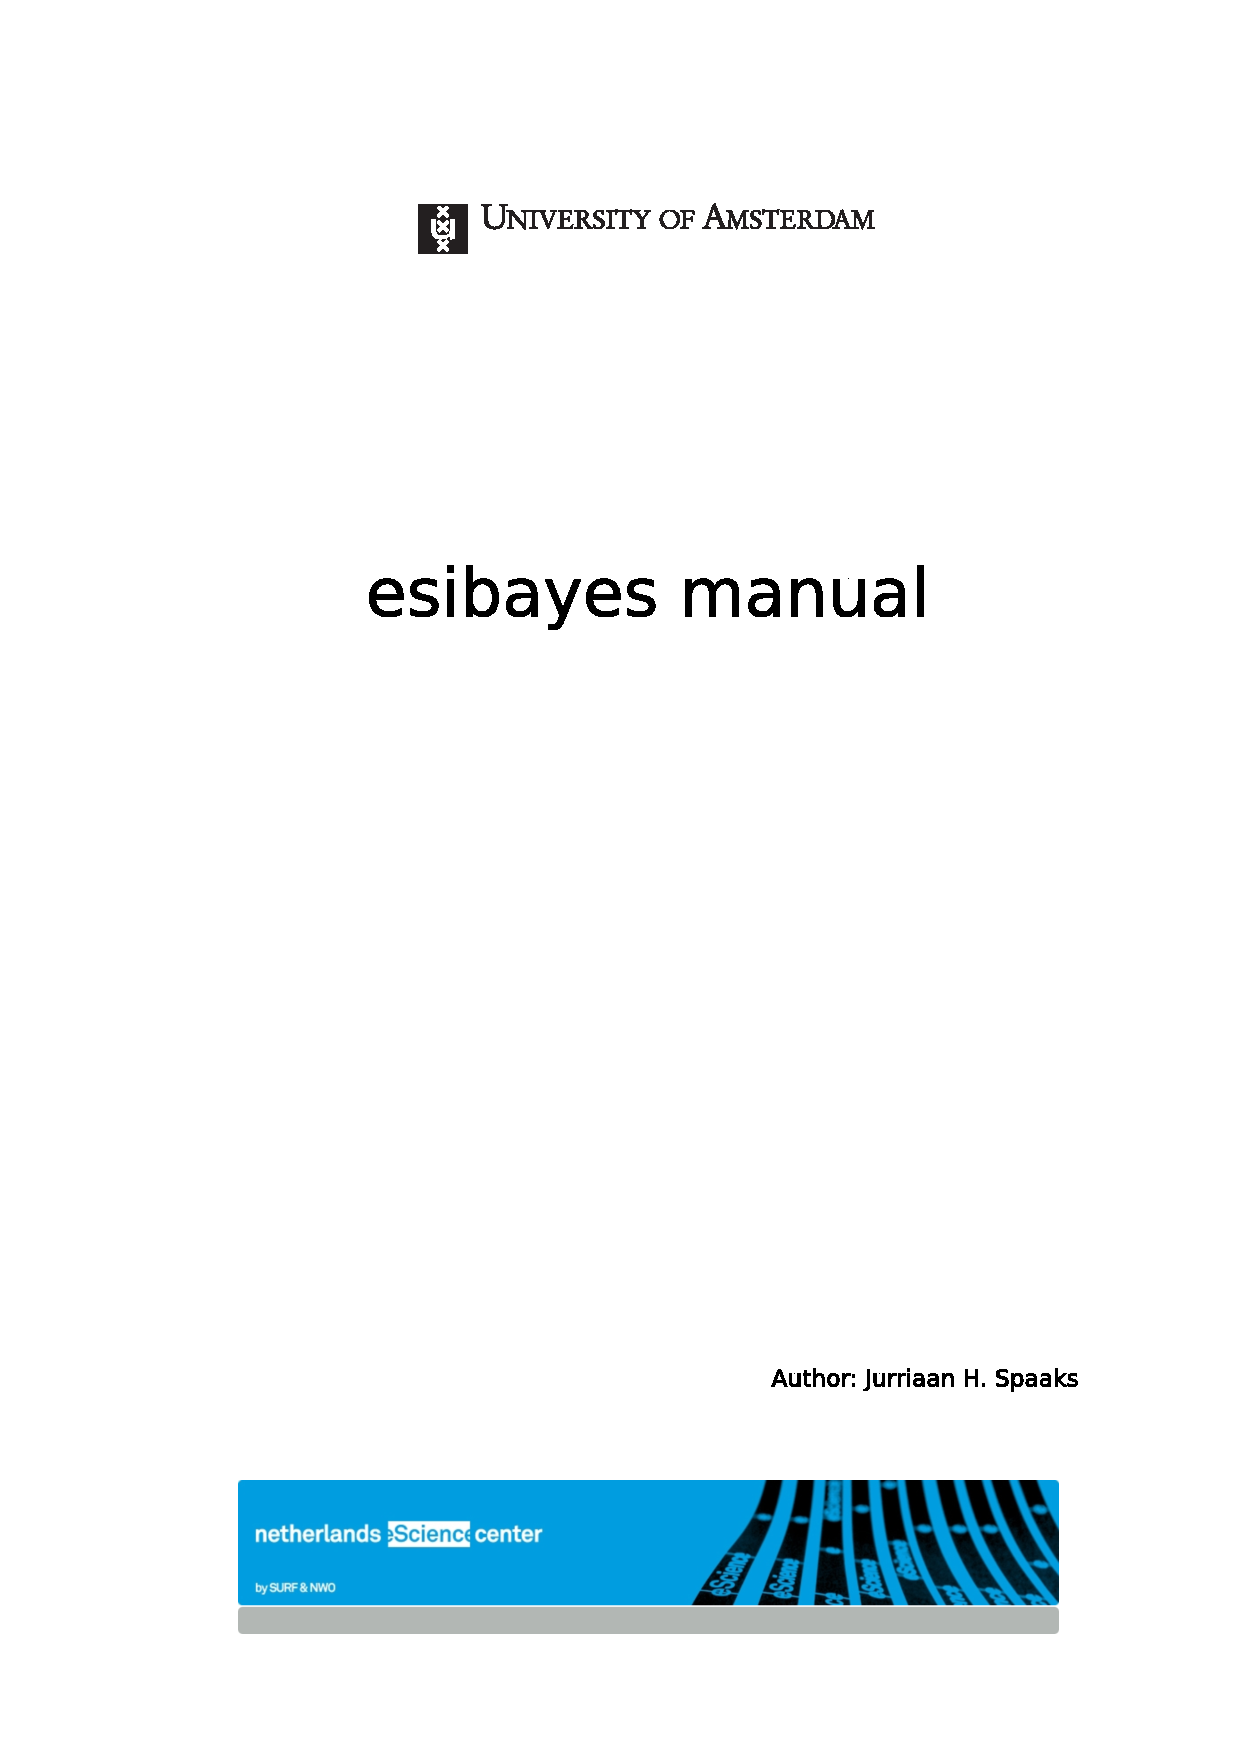
\includegraphics{./../eps/esibayes-manual-front}}%
}
 
\end{titlepage}

\insertemptypage{}
\insertemptypage{}

\pagestyle{plain}
\frontmatter

\tableofcontents
%\newpage

\mainmatter
\chapter{Introduction}
%\thispagestyle{fancy}
\label{ch:introduction}


This document is a manual for learning how to use the LISA cluster computer hosted at SARA (\burl{https://www.surfsara.nl/systems/lisa}) for solving parameter tuning and system identification problems. The manual covers the basic organization of the cluster's hardware, and provides the user with some simple commands you'll need for manipulating the Linux system that LISA is running. The manual further introduces the MMSODA parameter tuning and system identification software that can be run on LISA. While going through this manual, you'll find that most of it is aimed at Windows users, but occasionally there will be brief instructions for Linux users as well (usually in the footnotes). It is assumed that you are proficient in using MATLAB. Furthermore, it is assumed that you have a basic understanding of some of the general concepts used in optimization.

\setcounter{smallqcounter}{0}

\chapter{Getting started}
\label{ch:getting-started}

Effective usage of the LISA system requires that you:
\begin{enumerate}
\item{have a basic understanding of how the LISA system is organized;}
\item{know how to copy files from your local machine to LISA and back using SFTP;}
\item{know how to establish an SSH connection, linking your local machine to the LISA system;}
\item{have a basic understanding of the Linux commands that are needed to tell the LISA system what it is you want to do.}
\end{enumerate}



\section{Cluster computing}

A \textit{cluster computer}\index{cluster computer} is a system of interconnected computers that work together so that in many respects they can be viewed as a single system. Clusters usually consist of regular \mbox{off-the-shelf} computers such as those you may find in any computer retail shop (see Fig.~\ref{fig:photo-cluster-computer-uchemnitz}). Cluster computers are especially suited for solving a certain class of computational problems, namely those problems that can be divided into smaller, independently solvable tasks. As a trivial example, finding the minimum value in a 2-D array of values (i.e. a map) is such a problem: the map can be split into two parts and sent to two separate machines. After both machines have found the minimum value in the part of the map that they were assigned, the `global' minimum can be determined by simply comparing the two values. Dividing the task over two or more machines (or actually, \textit{cores}\index{core}) is called \textit{parallelization}\index{parallelization}. Parallelization can greatly reduce the \textit{walltime}\index{walltime} of a computational task (i.e. the time between starting a task and knowing the solution). 

\begin{figure}[htb]
  \centering
    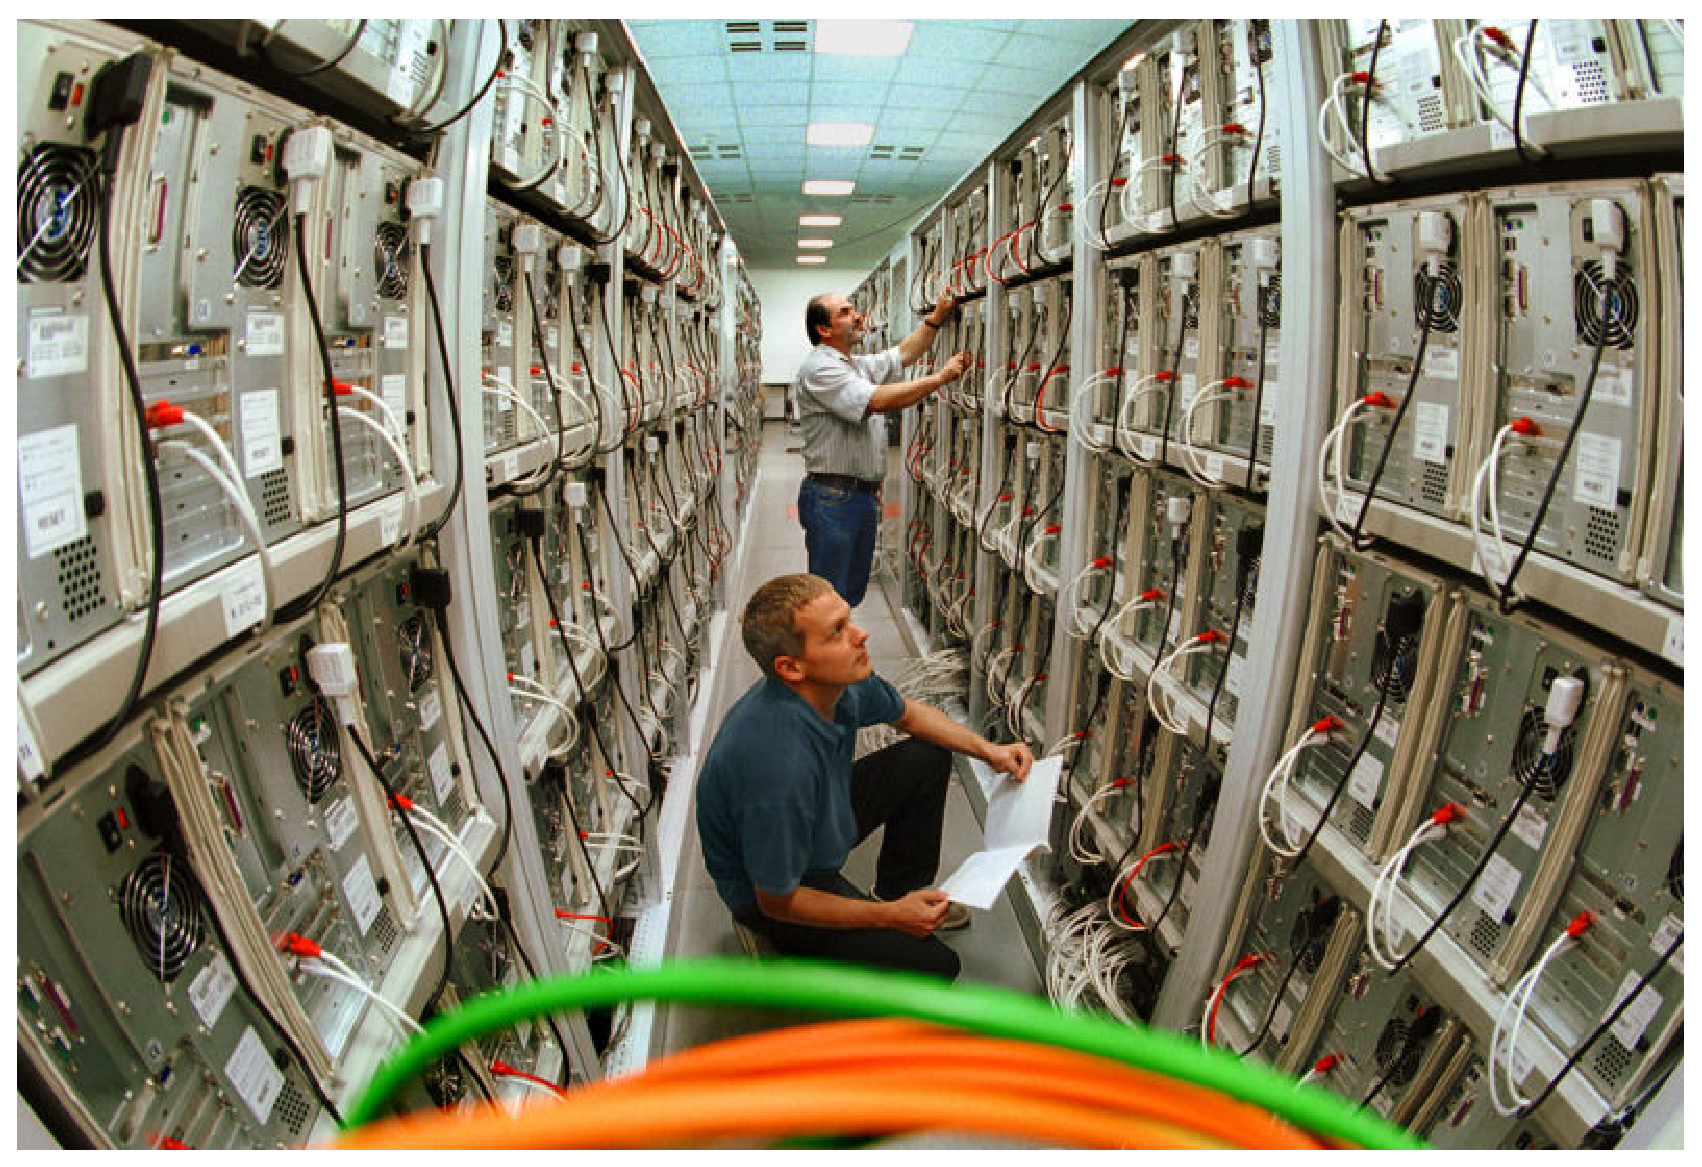
\includegraphics[width=\textwidth]{./../eps/photo-cluster-computer-uchemnitz.eps}
  \caption{Technicians at work on a real cluster computer. Photo from \burl{http://en.wikipedia.org/wiki/File:MEGWARE.CLIC.jpg}.}
  \label{fig:photo-cluster-computer-uchemnitz}
\end{figure}


\section{The LISA cluster: hardware}\index{LISA}

The LISA cluster currently\footnote{LISA's hardware is subject to regular upgrades. For concurrent information, see \burl{https://www.sara.nl/systems/lisa/description\#System_configuration}} consists of 624 normal computers, which are referred to as \textit{nodes}\index{node}. In terms of hardware, each node has a Central Processing Unit (CPU), disk storage, and memory. The nodes are interconnected using a Local Area Network (LAN\index{LAN}). The LAN has low latency and high bandwidth (Gigabit\index{Gigabit} or Infiniband\index{Infiniband}), meaning that in terms of time it is cheap to send large files (because of the high bandwidth) as well as small files (because of the low latency). Storage space on each node varies a little bit, but at the time of writing is 70--220 GB per node. Most nodes have 8-core CPUs, although some have 12-cores or 16-cores. The clock frequency for individual cores is 1.80--2.26 GHz. In terms of memory, most nodes have 24 GB, but the 16-cores have 32 GB. Furthermore, the bandwidth between memory and CPU varies between 5.86--8.00 GT/s. Finally, all nodes run the Debian Linux AMD64 operating system.



\section{Transferring files to and from the LISA cluster}

This section documents the necessary steps for connecting to the LISA cluster from a local Windows machine. First, make sure that you have an account for accessing LISA\footnote{You can get an account by following the instructions from \url{https://www.sara.nl/systems/lisa/account}}. In order to use the cluster effectively, you need to be able to copy files to and from your user directory on the cluster. The LISA cluster is set up such that it exclusively allows connections that are secure, such as Secure File Transfer Protocol (SFTP\index{SFTP}) connections or Secure Shell (SSH\index{SSH}) connections. There are many programs that can establish secure connections, but we will use WinSCP\index{WinSCP}.

Download WinSCP from \burl{http://sourceforge.net/projects/winscp/files/WinSCP/4.3.7/winscp437.zip/download}\footnote{By the time you read this, there may be a more recent version available---just substitute `4.3.7' and `437' from the address with the version you want. For an overview of available versions, look here: \burl{http://sourceforge.net/projects/winscp/files/WinSCP/}.}\footnote{Life is somewhat easier for Linux users. Most Linux distributions come with built-in support for secure connections. Just start up your regular file browser (e.g. PCManFM, Thunar, Nautilus, etc) and type in the address bar \burl{sftp://jspaaks@lisa.sara.nl/home/jspaaks}. Don't forget to substitute your own username. This should automatically establish a connection between your machine and the remote system (i.e. the cluster). Fill in your credentials when prompted.}. Unzip into your home directory or a USB drive. Double-click on `WinSCP.exe' to start the WinSCP program. The program will prompt you for some input (see Fig.~\ref{fig:winscp-session-dialog}). Under `Host name:', fill in `lisa.sara.nl'. Make sure that the port number is set to `22'. Under `User name:', fill in your LISA cluster username. You can leave the `Password' field blank, the program will prompt you later. Make sure `SFTP' is selected as the file protocol. Click on `Save...' to store these settings if you like. Then press the `Login' button to establish the SFTP connection to the LISA cluster. The program will throw a warning about the RSA key fingerprint file. The number shown in the warning dialog should be the same as the number posted at \burl{https://www.sara.nl/systems/shared/ssh} (table at the bottom of the web page). If it is, press `Yes' and then `Continue' in the next dialog box. As a final step, fill in your password when prompted. You should now see two panes, one for the local machine on the left and one for the remote machine, i.e. the LISA cluster, on the right (see Fig.~\ref{fig:winscp-two-panes}).

\begin{figure}[htbp]
  \centering
    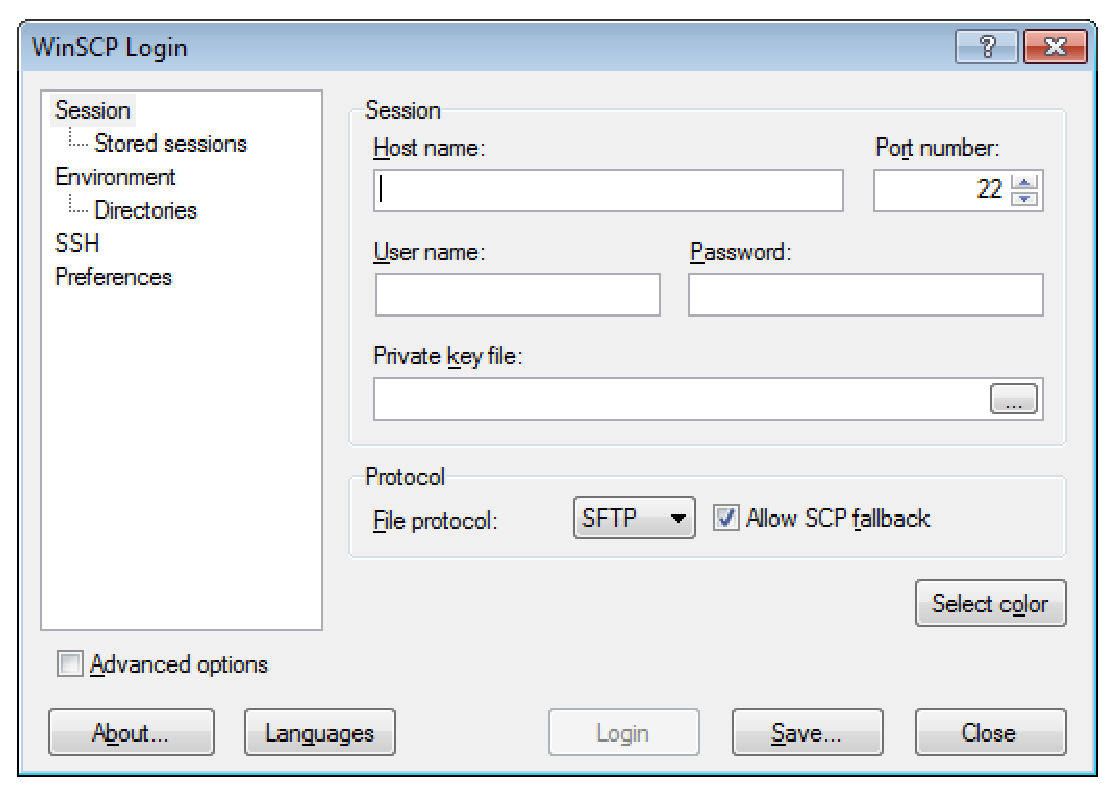
\includegraphics[width=0.5\textwidth]{./../eps/winscp-session-dialog.eps}
  \caption{WinSCP session dialog box.}
  \label{fig:winscp-session-dialog}
\end{figure}

\begin{figure}[htbp]
  \centering
    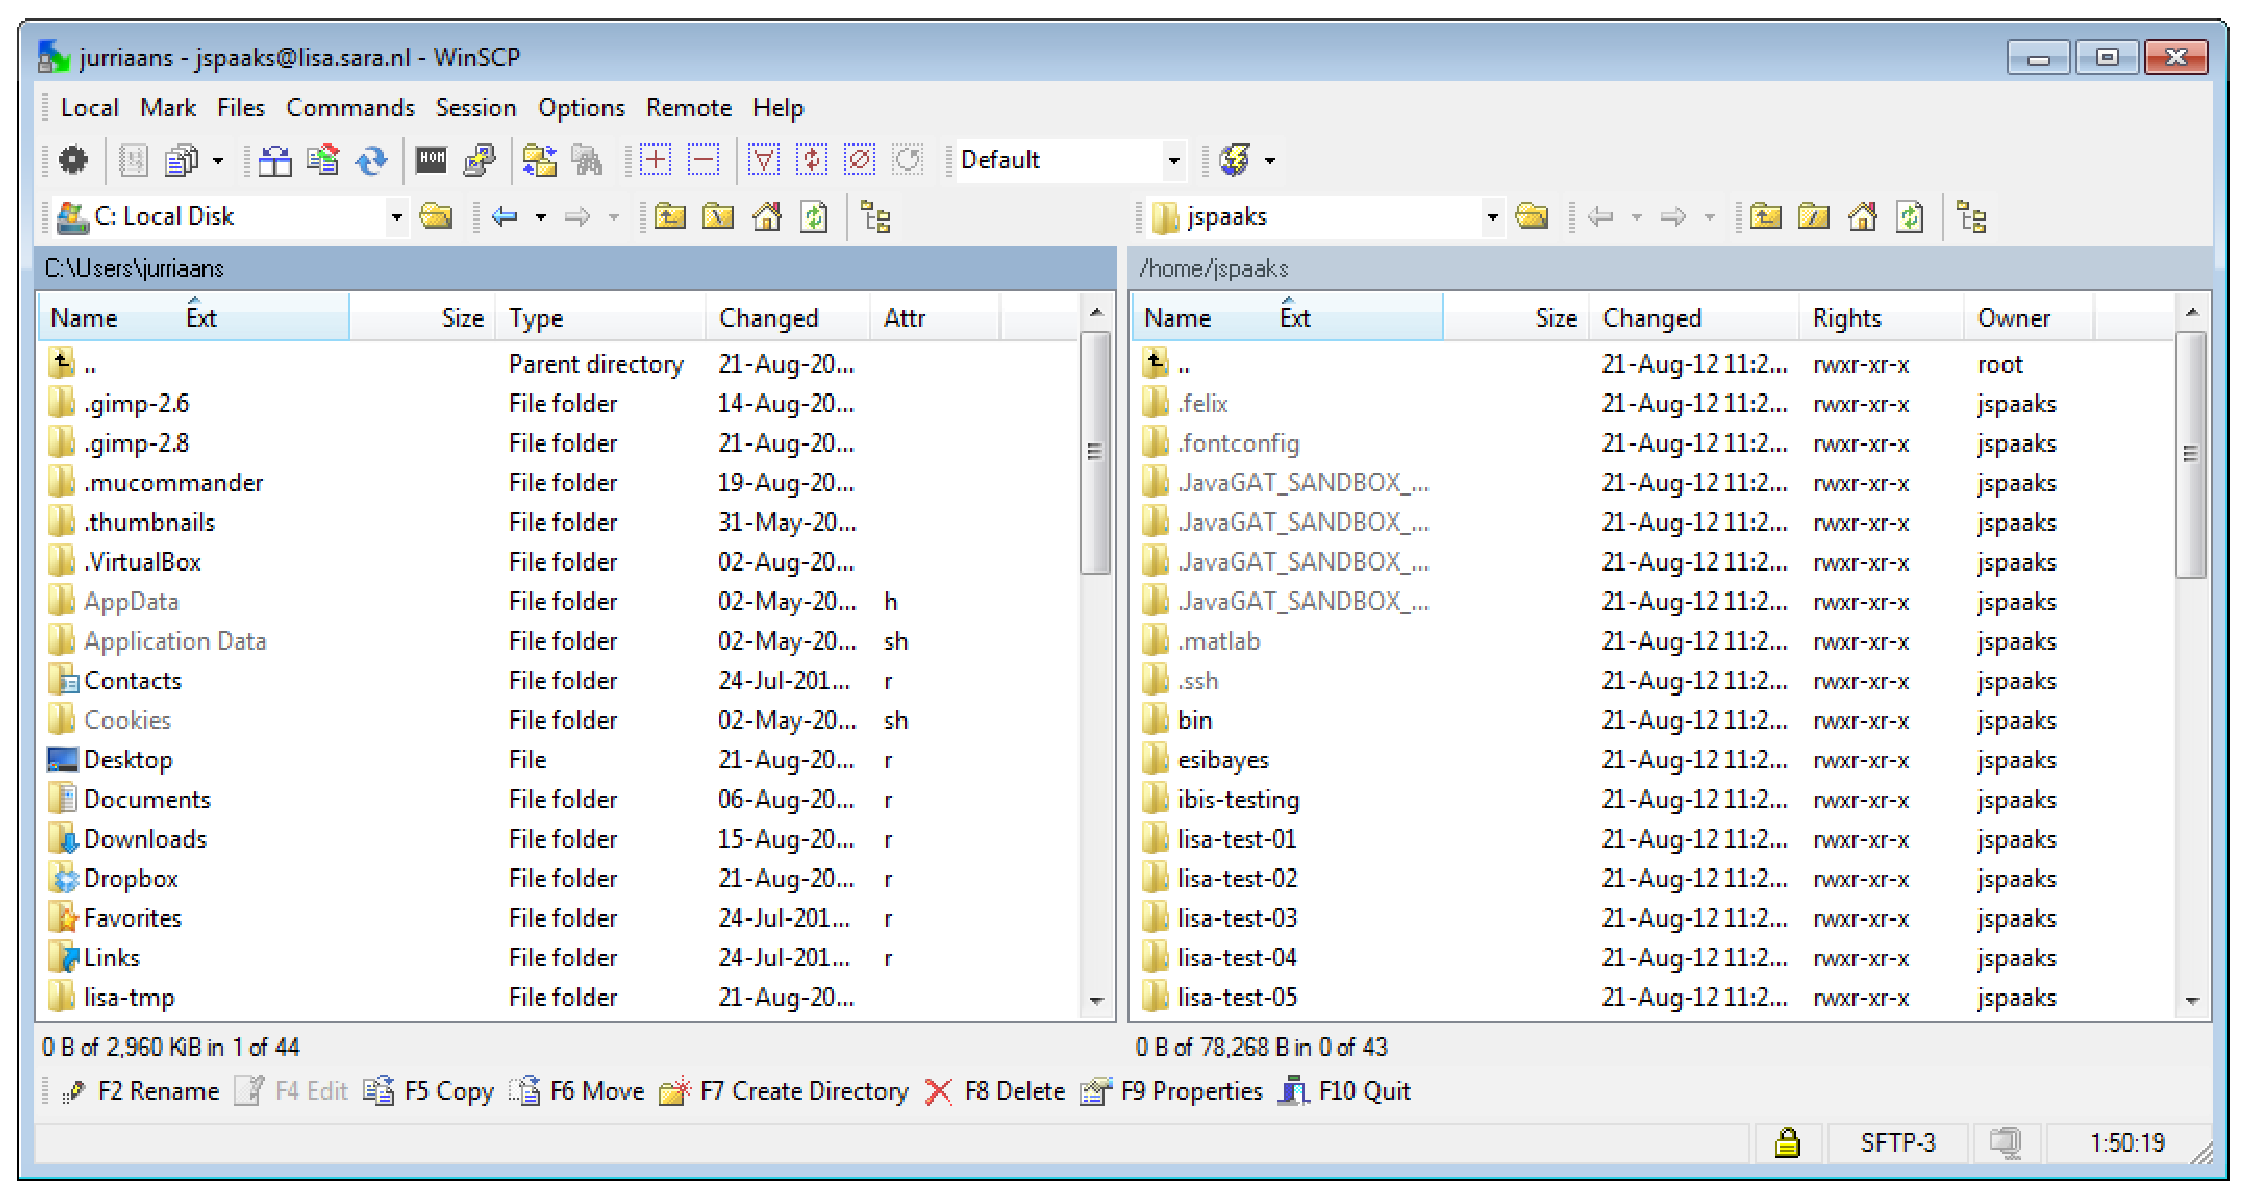
\includegraphics[width=1.0\textwidth]{./../eps/winscp-two-panes.eps}
  \caption{WinSCP interface. On the left is my local file system, on the right is my home directory on the remote file system. If this is the first time you connect to LISA, the remote file system should be pretty much empty.}
  \label{fig:winscp-two-panes}
\end{figure}

Download `tutorial.zip' from \url{http:\\www.????.??} and unzip into your (local) home directory or a USB drive.

In WinSCP, use the left pane to navigate to the directory where you unzipped the tutorial files. Copy the `tutorial' folder to the remote directory by selecting it on the left and pressing the F5 button. The tutorial folder should now be present in the right pane as well.


\section{Issuing commands on the LISA cluster}
This section covers how you can issue commands from your local machine, which then get executed by the remote system (LISA). Issuing commands on the LISA cluster can be accomplished through a so-called terminal emulator program\index{terminal emulator}. A terminal emulator provides you with a prompt at which you can type commands which are then executed on the remote system. It doesn't matter whether the remote system is located just across the street or halfway around the world, you can still operate it through the terminal emulator. However, it is important to note that the LISA cluster, like virtually all clusters\footnote{See \burl{http://i.top500.org/stats} for concurrent statistics on the World's top 500 of supercomputers.}, runs under the Linux operating system. The commands that you type at the terminal emulator prompt therefore need to be Linux commands, which, as you will see later, are somewhat different from the Windows commands that you may be familiar with.

%
Let's first download the terminal emulator PuTTY\index{PuTTY} from \url{http://www.chiark.greenend.org.uk/~sgtatham/putty/download.html} into your home directory. Double-click the executable to run the program. You should now see the dialog from Fig.~\ref{fig:putty-session-dialog}. Under `Host name or IP address', fill in `lisa.sara.nl' and press the `Open' button. PuTTY first prompts you for your username and then for your password. Fill in your LISA credentials.\footnote{On Linux, bring up a terminal (Ctrl-Alt-t on most distributions) and type in \texttt{ssh jspaaks@lisa.sara.nl}, substituing your own username in stead of \texttt{jspaaks}. Fill in your credentials when prompted.}

\begin{figure}[htbp]
  \centering
    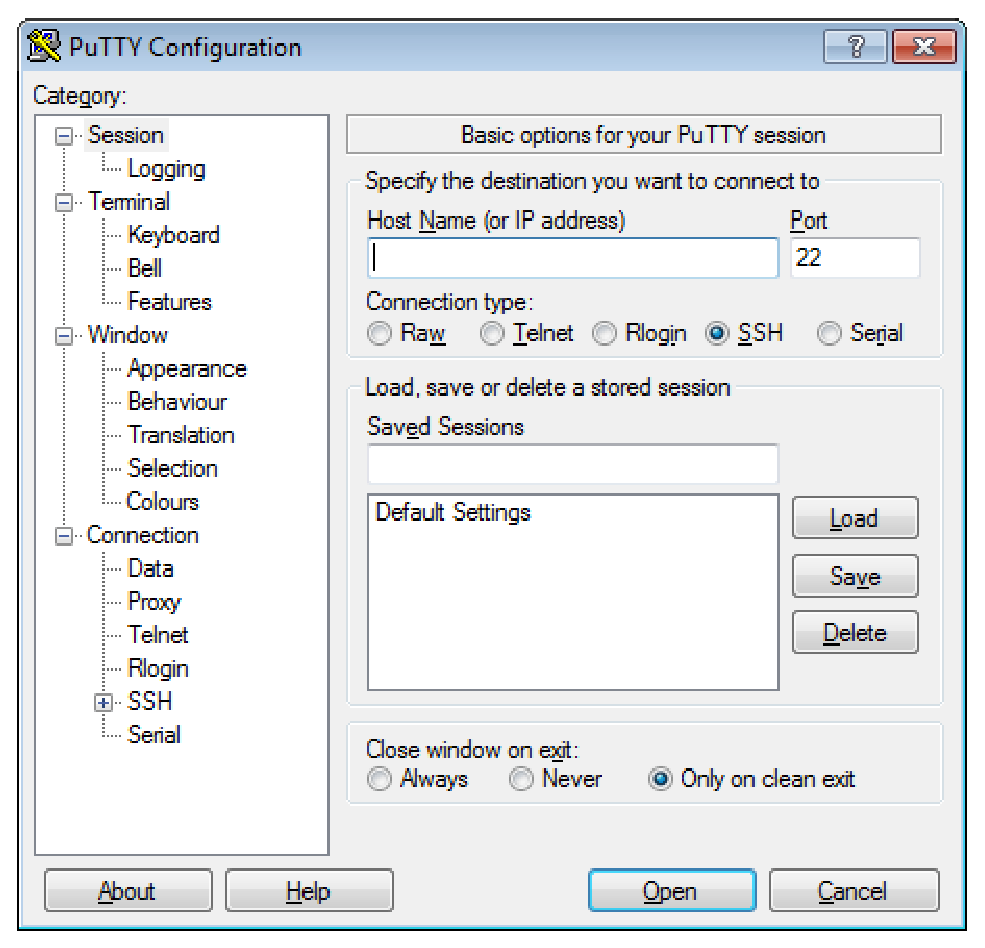
\includegraphics[width=0.5\textwidth]{./../eps/putty-session-dialog.eps}
  \caption{PuTTY session dialog box.}
  \label{fig:putty-session-dialog}
\end{figure}


You are now remotely logged in to the Linux cluster LISA. Your terminal emulator program should show something like:
\begin{lstlisting}[style=basic,style=bash]
jspaaks@login4:~$
\end{lstlisting}
where \texttt{jspaaks} is the username and \texttt{login4}\index{login4@\texttt{login4}} is the name of the remote machine. There are, in fact, two machines on which you can log in remotely: besides \lstinline[style=bashinline]{login4}, there's also \lstinline[style=bashinline]{login3}\index{login3@\texttt{login3}}. For our intents and purposes, it doesn't matter whether you are logged in to \lstinline[style=bashinline]{login3} or \lstinline[style=bashinline]{login4}, but if you want to change from one to the other, you can do so with:
\begin{lstlisting}[style=basic,style=bash]
jspaaks@login4:~$ ssh login3
\end{lstlisting}

When you're done with the terminal, you can close the connection using: 
\index{Linux commands!logout@\texttt{logout}}
\begin{lstlisting}[style=basic,style=bash]
jspaaks@login4:~$ logout
\end{lstlisting}


If you want to find out in which directory you are, you can use the \lstinline[style=bashinline]{pwd}\index{Linux commands!pwd@\texttt{pwd}} command (`pwd' is short for present working directory):
\begin{lstlisting}[style=basic,style=bash]
jspaaks@login4:~$ pwd
\end{lstlisting}
which returns:
\begin{lstlisting}[style=basic,style=bash]
/home/jspaaks
\end{lstlisting}
It is worth noting that a list of useful commands and terms has been included in the Index section at the back of this document.

So, \texttt{pwd} returns \texttt{/home/jspaaks/}. \texttt{/home/jspaaks/} is the user's home directory; it is the Linux equivalent of `C:\textbackslash{}Users\textbackslash{}jspaaks' on Windows. Note that on Linux the directory separator \index{/@\texttt{/} (directory separator, Linux)} is the forward slash `/' sign, whereas~Windows uses the backslash `\textbackslash{}'\index{\textbackslash{}@\texttt{\char`\\
} (directory separator, Windows)} sign. You may be wondering why there isn't a `C:\textbackslash{}' in the address returned by \texttt{pwd}. The reason is simple: Linux uses `/'\index{/@\texttt{/} (file system root, Linux)}\index{root@root (file system)} instead of `C:\textbackslash{}' \footnote{Somewhat confusingly, the account that has Administrator privileges is also referred to as `root' on Linux systems.\index{root@root (system administrator)}}. The first forward slash in the address is referred to as the `file system root'. Under the file system root is a directory `home', which contains a subdirectory `jspaaks' in which the user `jspaaks' keeps all his personal files. As a matter of fact, \texttt{/home/jspaaks} is the only place on this file system that user `jspaaks' is permitted to write anything, meaning that Linux will not allow you to save any files in other users' home directories (although you are allowed to read some of them, depending on how the \textit{permissions}\index{permission} on that directory are set. More about permissions later).

You can view the contents of the current directory using the \texttt{ls} (short for `list') command:\index{Linux commands!ls@\texttt{ls}}
\begin{lstlisting}[style=basic,style=bash]
jspaaks@login4:~$ ls
\end{lstlisting}
This should show at least the `tutorial' folder that we just copied using WinSCP.

Changing the current working directory works in a similar way as at the Command Prompt on Windows:
\begin{lstlisting}[style=basic,style=bash]
jspaaks@login4:~$ cd tutorial
jspaaks@login4:~/tutorial$ 
\end{lstlisting}\index{Linux commands!cd@\texttt{cd}}
Note that the prompt includes the location of the current directory: `\textasciitilde' (pronounced: `tilde') represents the home directory (`/home/jspaaks').
Changing to the current working directory from any location on the file system to the user's home directory goes like so:
\begin{lstlisting}[style=basic,style=bash]
jspaaks@login4:~/tutorial/a/really/deeply/nested/directory$ cd ~
jspaaks@login4:~$ 
\end{lstlisting}
or if you want to move just one directory up:
\begin{lstlisting}[style=basic,style=bash]
jspaaks@login4:~/tutorial/a/really/deeply/nested/directory$ cd ..
jspaaks@login4:~/tutorial/a/really/deeply/nested$ 
\end{lstlisting}
make sure to include the space character in between the \texttt{cd} and \texttt{..} characters though, otherwise it won't work.

A new directory can be created by the \texttt{mkdir}\index{Linux commands!mkdir@\texttt{mkdir}} command, for example:
\begin{lstlisting}[style=basic,style=bash]
jspaaks@login4:~$ mkdir anewdir
\end{lstlisting}\index{Linux commands!mkdir@\texttt{mkdir}}
Note that, contrary to Windows file systems, Linux file systems are case-sensitive. For example:
\begin{lstlisting}[style=basic,style=bash]
jspaaks@login4:~$ mkdir aNewDir
\end{lstlisting}
will result in an additional directory:
\begin{lstlisting}[style=basic,style=bash]
jspaaks@login4:~$ ls
anewdir   aNewDir   tutorial
jspaaks@login4:~$ 
\end{lstlisting}
The different approaches that Windows and Linux take in regard to case-sensitivity of their respective file systems can lead to errors, especially when copying back and forth between Windows and Linux systems. For example, the contents of \lstinline{anewdir} and \lstinline{aNewDir} may get merged when they are copied to a Windows system, since Windows regards the folders as being one and the same. To avoid these kinds of errors, the naming convention on Linux is to use only lower caps names for files and folders, so \lstinline{anewdir} is preferable to  \lstinline{aNewDir}. 

Regardless of your native operating system, your code will be more robust and more portable if you stick to these 2~simple rules when naming your files:
\begin{enumerate}
\item{don't use spaces;}
\item{limit yourself to the following subset of characters:\\ \lstinline[style=bashinline]{abcdefghijklmnopqrstuvwxyz_-.0123456789},\\ and, if you must, \lstinline[style=bashinline]{ABCDEFGHIJKLMNOPQRSTUVWXYZ} .}\footnote{You'll thank me later!}
\end{enumerate}



Removing a directory goes like this:
\begin{lstlisting}[style=basic,style=bash]
jspaaks@login4:~$ rmdir aNewDir
\end{lstlisting}\index{Linux commands!rmdir@\texttt{rmdir}}
or like this if you want to remove multiple directories:
\begin{lstlisting}[style=basic,style=bash]
jspaaks@login4:~$ rmdir anewdir aNewDir 
\end{lstlisting}


For many commands, you can specify options. Options to a given command must generally be provided directly after the command itself, i.e.~before any other argument such as input or output files.  The option argument consists of one dash followed by one (case-sensitive) letter. For example, if you want \texttt{ls} to list the contents of the current directory in more detail, you can use the \texttt{-l} option (that is the letter~\textit{l} for `long', not the number~1):
\begin{lstlisting}[style=basic,style=bash]
jspaaks@login4:~$ ls -l
total 4
drwxrwxr-x 2 jspaaks jspaaks 2 Jun 13 13:07 tutorial
\end{lstlisting}
which gives you, amongst other things, the \textit{permission bits}\index{permission bits} (i.e.\,\lstinline{drwxrwxr-x}), the owner of the item (\lstinline{jspaaks}), the item's size (\lstinline{2}) in bytes and the time when the item was last altered (\lstinline{Jun 13 13:07}). Note that, by default, \lstinline[style=bashinline]{ls} sorts the items in a directory based on the item's name, so directories and files will appear intermingled. You can easily tell whether an item is one or the other by looking at the permission bits: if the item is a folder, the first character that appears in the permission bits is the letter \lstinline[style=bashinline]{d}. For files, the first character in the permission bits is \lstinline[style=bashinline]{-}.

Most Linux commands have at least a few optional arguments. If you want to know more about a particular command's usage, you can use the \texttt{man}\index{Linux commands!man@\texttt{man}} (short for `manual') command, which lists all the options for a given program including a short description of what each option does. For example, try:
\begin{lstlisting}[style=basic,style=bash]
jspaaks@login4:~$ man ls
\end{lstlisting}
(you can scroll down using the `Up' and `Down' arrows. Pressing the `q' key lets you return to the prompt). If you just want to verify that you remember the command right, you can check by: 
\begin{lstlisting}[style=basic,style=bash]
jspaaks@login4:~$ whatis ls
ls (1)               - list directory contents
\end{lstlisting}
which will give you a short summary of what \lstinline{ls} is doing, but without all the technical detail.

In addition to the shorthand notation, some options also have a longer version for improved readibility. The longer version always starts with two dashes instead of one. As an example, the \lstinline[style=bashinline]{-h} option makes \lstinline[style=bashinline]{ls} list the filesizes in more easily interpretable units such as kB or MB, rather than in bytes:
\begin{lstlisting}[style=basic,style=bash]
jspaaks@login4:~$ ls -l -h
\end{lstlisting}
or, combining the shorthand options:
\begin{lstlisting}[style=basic,style=bash]
jspaaks@login4:~$ ls -lh
\end{lstlisting}
The longer version of the \lstinline[style=bashinline]{-h} option is \lstinline[style=bashinline]{--human-readable}, so the complete command becomes: 
\begin{lstlisting}[style=basic,style=bash]
jspaaks@login4:~$ ls -l --human-readable
\end{lstlisting}


Now that you know a little bit about Linux, let's look at how to manipulate files. \lstinline[style=bashinline]{cd} into the `deeply nested directory' by typing:
\begin{lstlisting}[style=basic,style=bash]
jspaaks@login4:~$ cd tu
\end{lstlisting}
if you now press Tab, the \textit{shell}\index{shell} program (i.e.\,the program that lets you enter commands at the prompt) will automatically complete your command, like so:\index{Linux commands!autocompletion}
\begin{lstlisting}[style=basic,style=bash]
jspaaks@login4:~$ cd tutorial
\end{lstlisting}
This autocomplete works because the shell knows that you want to do a \lstinline[style=bashinline]{cd}, and since there is only one directory in \textasciitilde{} that starts with \lstinline[style=bashinline]{tu}, the shell program knows that you want to \lstinline[style=bashinline]{cd} into \lstinline[style=bashinline]{tutorial}.

If you \lstinline[style=bashinline]{cd} into \lstinline{a/really/deeply/nested/directory} and list the directory contents, there should be a file called `with-a-file-in-it.txt'. Because this is an \mbox{ASCII} text file, you can display it in the shell program by using the command \lstinline[style=bashinline]{cat}\index{Linux commands!cat@\texttt{cat}}, like so:
\begin{lstlisting}[style=basic,style=bash]
jspaaks@login4:~/tutorial/a/really/deeply/nested/directory$ cat with-a-file-in-it.txt
\end{lstlisting}

\lstinline[style=bashinline]{cat} is short for `concatentate', meaning it appends the contents of `with-a-file-in-it.txt' to whatever is already displayed within the shell. Also note that autocomplete works here as well, but instead of listing any directory names, it will suggest a file from the current directory, since that is the kind of argument that \lstinline[style=bashinline]{cat} expects. You will see the following output:
\begin{lstlisting}[style=basic,style=bash]
jspaaks@login4:~$ cd tutorial/a/really/deeply/nested/directory/
jspaaks@login4:~/tutorial/a/really/deeply/nested/directory$ ls
with-a-file-in-it.txt
jspaaks@login4:~/tutorial/a/really/deeply/nested/directory$ cat with-a-file-in-it.txt 
* * * * * * * * * * * * * * * * * * * * *
* *                                   * *
* *  hello world, the classic phrase  * *
* *                                   * *
* * * * * * * * * * * * * * * * * * * * *
jspaaks@login4:~/tutorial/a/really/deeply/nested/directory$ 
\end{lstlisting}
(the lines that start with asterisks are actually the contents of `with-a-file-in-it.txt'.)

Let's now try to move this file to the top directory in the user's home by using the move command \lstinline[style=bashinline]{mv}\index{Linux commands!mv@\texttt{mv}}\index{Linux commands!move} like so:
\begin{lstlisting}[style=basic,style=bash]
jspaaks@login4:~/tutorial/a/really/deeply/nested/directory$ mv with-a-file-in-it.txt ~
\end{lstlisting}
The syntax for this command is the command itself, i.e.~\lstinline[style=bashinline]{mv}, followed by a space, followed by the first input argument, in this case the name of the file that we want to move, i.e.~\lstinline[style=bashinline]{with-a-file-in-it.txt}, followed by another space, followed by the name of the directory that we want to move it to \lstinline[style=bashinline]{~}. Also note that autocomplete works here as well, just type \lstinline[style=bashinline]{mv wit} and press Tab to autocomplete.

Let's check that the file really got moved:
\begin{lstlisting}[style=basic,style=bash]
jspaaks@login4:~/tutorial/a/really/deeply/nested/directory$ cd ~
jspaaks@login4:~$ ls -l
total 6
drwxr-xr-x  4 jspaaks jspaaks    4 Aug 20 11:59 tutorial
-rw-r--r--  1 jspaaks jspaaks  210 Aug 20 15:21 with-a-file-in-it.txt
jspaaks@login4:~$  
\end{lstlisting}

You can also use the \lstinline[style=bashinline]{mv} command to rename\index{Linux commands!rename} a file by `moving' it to a different filename in the same directory like so:
\begin{lstlisting}[style=basic,style=bash]
jspaaks@login4:~$ ls -l
total 6
drwxr-xr-x  5 jspaaks jspaaks    5 Aug 21 14:45 tutorial
-rw-r--r--  1 jspaaks jspaaks  210 Aug 20 15:21 with-a-file-in-it.txt
jspaaks@login4:~$ mv with-a-file-in-it.txt the-renamed-file.txt 
jspaaks@login4:~$ ls -l
total 6
-rw-r--r--  1 jspaaks jspaaks  210 Aug 20 15:21 the-renamed-file.txt
drwxr-xr-x  5 jspaaks jspaaks    5 Aug 21 14:45 tutorial
jspaaks@login4:~$ 
\end{lstlisting}


Now suppose we don't want to move a file but we want to copy it. This can be done using the \lstinline[style=bashinline]{cp}\index{Linux commands!cp@\texttt{cp}}\index{Linux commands!copy} command. For example:
\begin{lstlisting}[style=basic,style=bash]
jspaaks@login4:~$ cp with-a-file-in-it.txt copy-of-the-text-file 
\end{lstlisting}
The copy command \lstinline[style=bashinline]{cp} expects the file-to-be-copied as its first argument, and the name of the file-to-copy-to as its second argument. Further note that you don't have to specify extensions such as `.txt' in the filename for the operating system to know that \lstinline[style=bashinline]{copy-of-the-text-file} is a text file, as you would normally do on Windows. Nevertheless, including the extension in the file name allows easy identification of the type of file, for example when listing the contents of a directory with \lstinline[style=bashinline]{ls}, especially when combined with wildcards such as \lstinline[style=bashinline]{*}:

\begin{lstlisting}[style=basic,style=bash]
jspaaks@login4:~/tutorial/a$ ls -l
total 10
-rw-rw-r-- 1 jspaaks jspaaks 16 Aug 22 10:02 file1.txt
-rw-rw-r-- 1 jspaaks jspaaks 16 Aug 22 10:00 file2.txt
-rw-rw-r-- 1 jspaaks jspaaks 16 Aug 22 10:00 file3.txt
-rw-rw-r-- 1 jspaaks jspaaks 13 Aug 22 10:02 file4.m
-rw-rw-r-- 1 jspaaks jspaaks 13 Aug 22 10:01 file5.m
drwxr-xr-x 3 jspaaks jspaaks  3 Aug 20 11:56 really
jspaaks@login4:~/tutorial/a$ ls -l *.txt
-rw-rw-r-- 1 jspaaks jspaaks 16 Aug 22 10:02 file1.txt
-rw-rw-r-- 1 jspaaks jspaaks 16 Aug 22 10:00 file2.txt
-rw-rw-r-- 1 jspaaks jspaaks 16 Aug 22 10:00 file3.txt
jspaaks@login4:~/tutorial/a$ 
\end{lstlisting}


\lstinline{cp} also lets you copy directories, like so:
\begin{lstlisting}[style=basic,style=bash,style=numbered]
jspaaks@login4:~$ cd tutorial
jspaaks@login4:~/tutorial$ ls -l
total 5
drwxr-xr-x 3 jspaaks jspaaks 3 Aug 20 11:56 a
drwxr-xr-x 2 jspaaks jspaaks 5 Aug 20 12:07 simple-jobscript
jspaaks@login4:~/tutorial$ mkdir another
jspaaks@login4:~/tutorial$ cp -R a/* another
jspaaks@login4:~/tutorial$ ls -l
total 8
drwxr-xr-x 3 jspaaks jspaaks 3 Aug 20 11:56 a
drwxrwxr-x 3 jspaaks jspaaks 3 Aug 21 14:46 another
drwxr-xr-x 2 jspaaks jspaaks 5 Aug 20 12:07 simple-jobscript
jspaaks@login4:~/tutorial$ cd another/really/deeply/nested/directory/
jspaaks@login4:~/tutorial/another/really/deeply/nested/directory$
\end{lstlisting}
Line 1 changes the current directory to \lstinline[style=bashinline]{tutorial}, line 2 lists its contents, line 6 creates the directory called `another'. The actual copying is subsequently done in line 7. The complete command consists of the \lstinline[style=bashinline]{cp} command, followed by the \lstinline[style=bashinline]{-R} option that makes \lstinline[style=bashinline]{cp} copy recursively, followed by the source files and folders \lstinline[style=bashinline]{a/*} (i.e.~everything under \lstinline[style=bashinline]{~/tutorial/a}), followed by the destination directory \lstinline[style=bashinline]{another}. Line 8 shows the newly created directory, while lines 13--14 show that the copy operation was indeed recursive.

Besides manipulating files and folders, the shell can do a lot more. For example, you can temporarily turn the shell program into a Octave\index{Octave} command window, like so:
\begin{lstlisting}[style=basic,style=bash]
jspaaks@login4:~$ octave
\end{lstlisting}
\index{Linux commands!octave@\texttt{octave}}

The Octave program welcomes you with its default welcome message, followed by a prompt:
\begin{lstlisting}[style=basic,style=bash]
GNU Octave, version 3.2.4
Copyright (C) 2009 John W. Eaton and others.
This is free software; see the source code for copying conditions.
There is ABSOLUTELY NO WARRANTY; not even for MERCHANTABILITY or
FITNESS FOR A PARTICULAR PURPOSE.  For details, type `warranty'.

Octave was configured for "x86_64-pc-linux-gnu".

Additional information about Octave is available at http://www.octave.org.

Please contribute if you find this software useful.
For more information, visit http://www.octave.org/help-wanted.html

Report bugs to <bug@octave.org> (but first, please read
http://www.octave.org/bugs.html to learn how to write a helpful report).

For information about changes from previous versions, type `news'.

octave:1> 
\end{lstlisting}
At the prompt, you can type any Octave command. For example: 
\begin{lstlisting}[style=basic,style=bash]
octave:1> for k=1:4, disp(['The value of ''k'' = ',num2str(k)]),end
The value of 'k' = 1
The value of 'k' = 2
The value of 'k' = 3
The value of 'k' = 4
octave:2> 
\end{lstlisting}
If you want to return to the normal shell, just type: 
\begin{lstlisting}[style=basic,style=bash]
octave:2> exit
\end{lstlisting}

From the example above, you can see that typing everything on the command line can be tricky, even for simple tasks. Wouldn't it be great to have an editor of some kind? You've guessed it, the shell can also be turned into a (very) basic editor, like so:
\begin{lstlisting}[style=basic,style=bash]
jspaaks@login4:~$ nano
\end{lstlisting}
\index{Linux commands!nano@\texttt{nano}}

You can use the nano program to write a simple Octave script, for example the one in Listing~\ref{list:nano-simple-script}:
\begin{lstlisting}[style=numbered,style=basic,style=bash,style=numbered,caption={Example of a simple Octave script in nano.},label=list:nano-simple-script]
  GNU nano 2.2.4                 New Buffer                                   Modified  

% This is a simple octave script example written in Nano

% clear any old variables
clear

for k=1:5
    str = ['The value of ''k'' is ',num2str(k)];
    disp(str)
end





^G Get Help    ^O WriteOut    ^R Read File   ^Y Prev Page   ^K Cut Text    ^C Cur Pos
^X Exit        ^J Justify     ^W Where Is    ^V Next Page   ^U UnCut Text  ^T To Spell
\end{lstlisting}
The first line of Listing~\ref{list:nano-simple-script} consists of the name and version of the nano program, followed by either the filename (if you opened an existing file) or the string \lstinline[style=bashinline]{New Buffer} (if the file has not been saved yet). The string \lstinline[style=bashinline]{Modified} is displayed at the right if the user has made any changes. The bottom two lines list a number of keyboard combinations, where the caret symbol~\lstinline[style=bashinline]{^} represents the Ctrl key, so \lstinline[style=bashinline]{^G} means Ctrl-g. After you've typed your script, you can save it by pressing Ctrl-o, typing the filename that you want your script to have, and pressing Enter. You can exit nano by pressing Ctrl-x. If you happen to press Ctrl-x when your script has not been saved yet, nano will ask you if you want to save it before exiting.

Let's check that the script from Listing~\ref{list:nano-simple-script} was written to file:
\begin{lstlisting}[style=basic,style=bash]
jspaaks@login4:~$ cat simple_octave_script.m 
% This is a simple octave script example written in Nano

% clear any old variables
clear

for k=1:5
    str = ['The value of ''k'' is ',num2str(k)];
    disp(str)
end
jspaaks@login4:~$ 
\end{lstlisting}

Now we can call the Octave program using the name of the script as an input argument like so:
\begin{lstlisting}[style=basic,style=bash]
jspaaks@login4:~$ octave simple_octave_script.m 
\end{lstlisting}
This starts the Octave program, runs the script within it as if you had typed `simple\_octave\_script' at the Octave prompt, and returns to the shell:
\begin{lstlisting}[style=basic,style=bash]
jspaaks@login4:~$ octave simple_octave_script.m 
GNU Octave, version 3.2.4
Copyright (C) 2009 John W. Eaton and others.
This is free software; see the source code for copying conditions.
There is ABSOLUTELY NO WARRANTY; not even for MERCHANTABILITY or
FITNESS FOR A PARTICULAR PURPOSE.  For details, type `warranty'.

Octave was configured for "x86_64-pc-linux-gnu".

Additional information about Octave is available at http://www.octave.org.

Please contribute if you find this software useful.
For more information, visit http://www.octave.org/help-wanted.html

Report bugs to <bug@octave.org> (but first, please read
http://www.octave.org/bugs.html to learn how to write a helpful report).

For information about changes from previous versions, type `news'.

The value of 'k' is 1
The value of 'k' is 2
The value of 'k' is 3
The value of 'k' is 4
The value of 'k' is 5

jspaaks@login4:~$ 
\end{lstlisting}

\section{Jobscripts and the scheduler}

So far, we've executed all our commands on just one machine, `login4'. As long as the task at hand is a small one, this isn't a problem, but if the task takes a long time to run, it can be advantageous to divide the task into smaller parts, and let each part be computed by a separate machine. The way this works on LISA is as follows: you write a small text file, referred to as a  \textit{jobscript}\index{jobscript} or \textit{batch file}\index{batch file}. The jobscript lays out the requirements of the task,  such as the number of nodes that is needed, the program that you want to run, and where the necessary data can be found. The jobscript is then sent to a program known as the \textit{scheduler}\index{scheduler}. The scheduler runs on LISA and manages the requests from all users, such that the computation resources are used in an optimal way, while taking into account things like different priority levels, the number and type of nodes that are needed, and so on. 

Listing~\ref{list:pbs-example-script} is an example of a simple jobscript.


\begin{lstlisting}[style=basic,style=bash,style=numbered,caption={Example of a jobscript.},label=list:pbs-example-script]
#PBS -lwalltime=00:01:00
#PBS -lnodes=1:cores8:ppn=1
#PBS -S /bin/bash

echo `date`: job starts

# run octave with the program:
octave --silent --no-window-system --eval "disp('hello world')"

echo `date`: job ends

exit
\end{lstlisting}

This jobscript asks the scheduler for a time slot of 1 minute (\lstinline[style=bashinline]{lwalltime=00:01:00}), and will be using one machine (\lstinline[style=bashinline]{lnodes=1}) with 8 cores in its CPU (\lstinline[style=bashinline]{cores8}). Only one of these cores will actually be doing something though, because the number of processes per node is just~1 (\lstinline[style=bashinline]{ppn=1}). The next line tells the scheduler that the rest of the jobscript is written in a scripting language called `bash'\index{bash}, which is a very common scripting language on Linux. As a matter of fact, you already know it, since the shell program you have been using is bash. The script then echoes the current date and time plus the message `: job starts' to the standard output\index{standard output} (more about standard input and standard output later).  Line 8 is the core of the script, in that it specifies what program needs to be run. In our case, it says that it wants to start an instance of the Octave software (\lstinline[style=bashinline]{octave}) and that this instance needs to be started with the \lstinline[style=bashinline]{--silent} and \lstinline[style=bashinline]{--no-window-system} options, such that it will not display the usual welcome message and that it will not use any of the graphical output methods (i.e.\, Octave's \lstinline[style=bashinline]{figure} command will not yield the usual output). The string following the \lstinline[style=bashinline]{--eval} option specifies the Octave command that will be run by the Octave software. Here, it is simply the \lstinline[style=bashinline]{disp('hello world')} command, but it could be any string that qualifies as valid Octave code, including function names and script names. The \lstinline[style=bashinline]{disp} command always writes to the standard output, which normally equates to saying that it outputs to your screen, but on the LISA system it actually is a file which we will check later. The script then echoes the current date and time plus the message `: job ends' to the standard output\index{standard output}, before exiting the script.

OK, so now that we have a jobscript file (which I saved as `\textasciitilde{}/tutorial/simple-batch/jobscript.pbs'---LISA uses the OpenPBS/Torque scheduler\footnote{http://www.adaptivecomputing.com/products/open-source/torque/}\index{OpenPBS}\index{PBS}\index{Torque}, so I usually save my jobscripts as *.pbs), let's send it to the scheduler with the \lstinline[style=bashinline]{qsub}\index{Linux commands!qsub@\texttt{qsub}} command (\lstinline[style=bashinline]{qsub} is an abbreviation for `submit to the queue'\index{scheduler!queue}, the queue in question being the scheduler's):
\begin{lstlisting}[style=basic,style=bash]
jspaaks@login4:~/tutorial/simple-batch$ qsub jobscript-slow.pbs
6388734.batch1.irc.sara.nl
jspaaks@login4:~/tutorial/simple-batch$ 
\end{lstlisting}
Note that I'm actually submitting a slightly different version of the jobscript here, which, as the name suggests, needs more time to finish. This is to make sure that the job runs sufficiently long for a user to check the job's statistics, because the LISA system can't show any statistics for jobs that are finished already.

As you can see above, \lstinline[style=bashinline]{qsub} prints a number \lstinline[style=bashinline]{6388734} to the shell. This number is referred to as the \textit{job id}\index{job id}.
You can check the status of the job by typing the \lstinline[style=bashinline]{qstat} command, followed by the job id, like so:
\begin{lstlisting}[style=basic,style=bash]
jspaaks@login4:~/tutorial/simple-batch$ qstat 6388734
Job id                    Name             User            Time Use S Queue
------------------------- ---------------- --------------- -------- - -----
6388734.batch1            ...ript-slow.pbs jspaaks                0 Q express        
jspaaks@login4:~/tutorial/simple-batch$ 
\end{lstlisting}
The \lstinline[style=bashinline]{S} column lists the \underline{s}tatus of the job. In this case, the job is queued, hence its status is listed in the table as \lstinline[style=bashinline]{Q}. Besides queued, it can be \lstinline[style=bashinline]{R}unning, \lstinline[style=bashinline]{C}ompleted, or \lstinline[style=bashinline]{H}eld. (There are a few more statuses which are more obscure, see \lstinline[style=bashinline]{man qstat}). \lstinline[style=bashinline]{qstat}'s \lstinline[style=bashinline]{-n} option shows the nodes that are allocated for your job (here: `gb-r2n14'):%,basicstyle=\tiny\ttfamily]

\begin{lstlisting}[style=basic,style=bash,xrightmargin=-10mm]
jspaaks@login4:~/tutorial/simple-batch$ qstat -u jspaaks -n

batch1.irc.sara.nl: 
                                                                         Req'd  Req'd   Elap
Job ID               Username Queue    Jobname          SessID NDS   TSK Memory Time  S Time
-------------------- -------- -------- ---------------- ------ ----- --- ------ ----- - -----
6388734.batch1.i     jspaaks  express  jobscript-slow.p  15291     1   1    --  00:01 R 00:00
   gb-r2n14/0
jspaaks@login4:~/tutorial/simple-batch$ 
\end{lstlisting}\index{Linux commands!qstat@\texttt{qstat}}
You can look up statistics for a given node at  \burl{https://ganglia.sara.nl/?r=hour&cs=&ce=&c=LISA+Cluster&h=gb-r2n14.irc.sara.nl&tab=m&vn=&mc=2&z=small&metric_group=ALLGROUPS}\index{Ganglia}, for example if you want to check its performance (see also Fig.~\ref{fig:ganglia-screenshot}).

Because \lstinline[style=bashinline]{6388734} is such a tiny job in terms of walltime and number of nodes, the scheduler adds the job to the `express queue'\index{queue!express}. Depending on the requirements layed out in the jobscript, your job may end up in one of 3 different queues:
\begin{enumerate}
\item{the express queue}\index{queue!express}
\item{the batch queue}\index{queue!batch}
\item{the interactive queue}\index{queue!interactive}
\end{enumerate}

\begin{figure}[hbt]
  \centering
    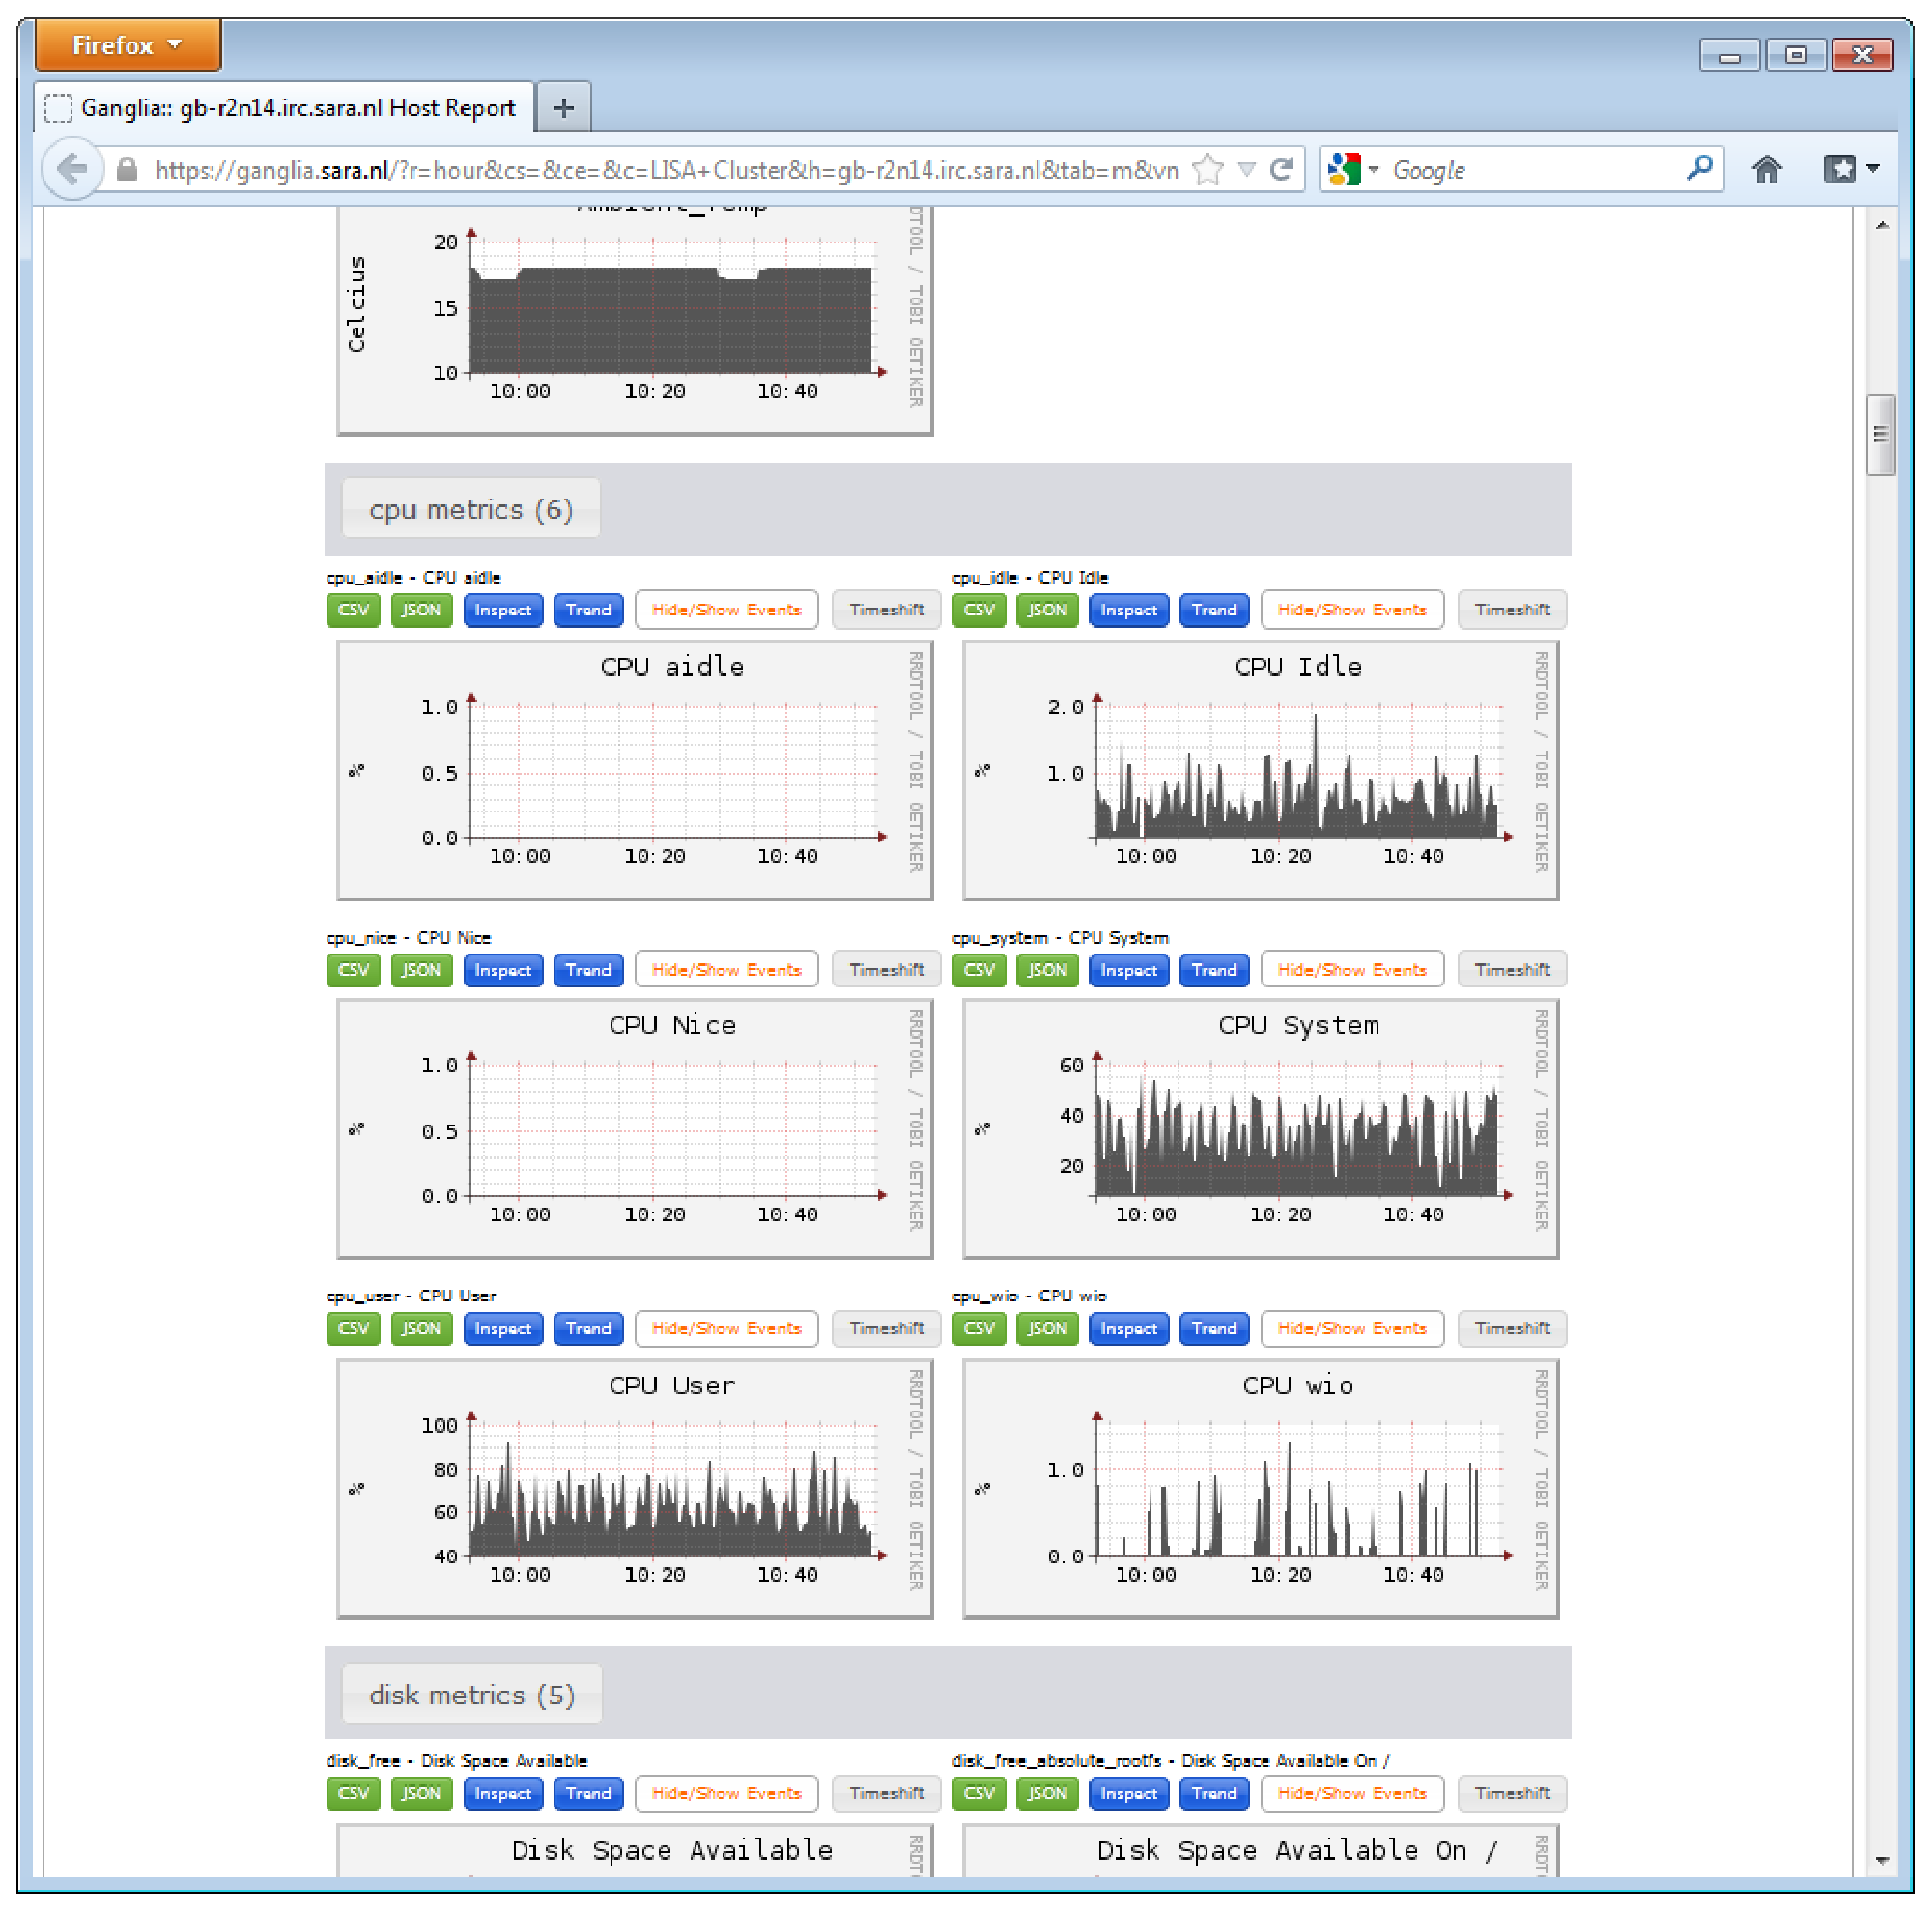
\includegraphics[width=0.9\textwidth]{./../eps/ganglia-screenshot.eps}
  \caption{Ganglia visualizes a wide array of performance indices for the LISA system. The plots can be viewed in a web browser such as Firefox.}
  \label{fig:ganglia-screenshot}
\end{figure}


Your job ends up in the express queue if it asks for less than 15~minutes walltime and doesn't use more than one node. If the system is not too busy, jobs in the express queue are usually executed without delay. In contrast, jobs that are in the batch queue can take a long time to start, but when they finally do, you can unleash the full computing power of the cluster. The interactive queue is primarily meant for development work that requires multiple machines. Submitting your job to the interactive queue is accomplished by the \lstinline[style=bashinline]{-I} option:
\begin{lstlisting}[style=basic,style=bash]
jspaaks@login4:~/tutorial$ qsub -I -lnodes=2:cores8:ppn=1 -lwalltime=00:03:00
qsub: waiting for job 6388157.batch1.irc.sara.nl to start
\end{lstlisting}
The above command asks for an interactive session with 2 nodes of the core8 type, each of which will only be running 1 process. Note that the information that is normally passed to \lstinline[style=bashinline]{qsub} through the first few lines in a jobscript (i.e.~the lines that start with \#PBS) must now be entered as options. After a delay, you will get a prompt on a different machine, in this case `gb-r7n32':

\begin{lstlisting}[style=basic,style=bash]
qsub: job 6388157.batch1.irc.sara.nl ready

jspaaks@gb-r7n32:~$ 
\end{lstlisting}
At this prompt, you can manually enter your commands, just like you were doing earlier, except you're no longer on `login4' anymore, but on one of the computing nodes within the cluster. When your time is up, the following message will appear:
\begin{lstlisting}[style=basic,style=bash]
jspaaks@gb-r7n32:~$ echo $PBS_O=>> PBS: job killed: walltime 215 exceeded limit 180
\end{lstlisting}
and you will return to `login4' (or `login3' if that's where you were before).

The \lstinline[style=bashinline]{showq} command lets you view (your part of) the queue, for example:\index{Linux commands!showq@\texttt{showq}}
\begin{lstlisting}[style=basic,style=bash]
jspaaks@login4:~/tutorial/simple-batch$ showq -u jspaaks
ACTIVE JOBS--------------------
JOBNAME            USERNAME      STATE  PROC   REMAINING            STARTTIME

6388079             jspaaks    Running     8    00:01:00  Thu Aug 23 15:41:24

     1 Active Job     6444 of 6684 Processors Active (96.41%)
                       617 of  647 Nodes Active      (95.36%)

IDLE JOBS----------------------
JOBNAME            USERNAME      STATE  PROC     WCLIMIT            QUEUETIME


0 Idle Jobs

BLOCKED JOBS----------------
JOBNAME            USERNAME      STATE  PROC     WCLIMIT            QUEUETIME


Total Jobs: 1   Active Jobs: 1   Idle Jobs: 0   Blocked Jobs: 0
jspaaks@login4:~/tutorial/simple-batch$ 
\end{lstlisting}
Also, \lstinline[style=bashinline]{showq} shows whether the cluster is very busy or not (Friday afternoons are usually the busiest, Mondays and Tuesdays are quiet in comparison). The statistics displayed by \lstinline[style=bashinline]{qsub} are updated every 15~seconds or so.


Some other commands that come in handy from time to time are:
\begin{lstlisting}[style=basic,style=bash]
jspaaks@login4:~/tutorial/simple-batch$ qdel 6388079
\end{lstlisting}\index{Linux commands!qdel@\texttt{qdel}}
This deletes job \lstinline[style=bashinline]{6388079} from the queue. Very useful if you accidentally requested too many nodes, or if your job crashed after like one second because you made a mistake. It's not possible to delete a job that was not submitted by you, so you don't have to worry about accidentally deleting other people's jobs if you type the job id wrong.

\vspace{1em}

\lstinline[style=bashinline]{checkjob} gives a more detailed overview of the job:\index{Linux commands!checkjob@\texttt{checkjob}}
\begin{lstlisting}[style=basic,style=bash]
jspaaks@login4:~/tutorial/simple-batch$ checkjob 6388672


checking job 6388672

State: Running
Creds:  user:jspaaks  group:lisa_uva  class:express  qos:DEFAULT
WallTime: 00:00:00 of 00:01:00
SubmitTime: Thu Aug 23 17:17:24
  (Time Queued  Total: 00:00:01  Eligible: 00:00:01)

StartTime: Thu Aug 23 17:17:25
Total Tasks: 1

Req[0]  TaskCount: 1  Partition: DEFAULT
Network: [NONE]  Memory >= 0  Disk >= 0  Swap >= 0
Opsys: [NONE]  Arch: x86_64  Features: [q_express][cores8]
Allocated Nodes:
[gb-r7n32:1]


IWD: [NONE]  Executable:  [NONE]
Bypass: 0  StartCount: 1
PartitionMask: [ALL]
Flags:       BACKFILL RESTARTABLE

Reservation '6388672' (00:00:00 -> 00:01:00  Duration: 00:01:00)
PE:  1.00  StartPriority:  -8641

jspaaks@login4:~/tutorial/simple-batch$ 
\end{lstlisting}

Finding out when your job is scheduled to start goes like this (the estimate is quite inaccurate in my experience):
\begin{lstlisting}[style=basic,style=bash]
showstart 6388079
\end{lstlisting}
\index{Linux commands!showstart@\texttt{showstart}}

\vspace{1em}



\chapter{Parallel optimization}


Optimization algorithms such as SCEM-UA \citep{vrug-gupt-bout-soro-2003}, SODA \citep{vrug-diks-gupt-bout-vers-2005}, Differential Evolution \citep{stor-pric-1997}, or DREAM \citep{vrug-terb-diks-robi-hyma-higd-2009} repeatedly sample the parameter space. In this chapter, we look at how such a sampling algorithm may be parallelized, and we introduce a law that describes the speedup that can be expected from parallelizing\index{parallel} a particular piece of software.

Most parameter optimization algorithms sample the parameter space in generations of independent samples. When the optimization is implemented as a \textit{serial }\index{serial} or \textit{sequential}\index{sequential} algorithm, the members of a generation are evaluated one after the other. For example, if the tasks that need to be evaluated each consist of one parameter set and there are 10 such tasks, the walltime that is needed to evaluate these tasks is equivalent to the sum of the CPU time that individual tasks need (Figure~\ref{fig:walltime-comparison}). In contrast, if the optimization algorithm employs a parallel strategy for evaluating the tasks, and the tasks are started simultaneously on 10 CPUs, then the walltime is determined by the CPU time of the slowest task (including the overhead introduced by the parallelization). The maximum speed-up $S$ that be gained from executing a task in parallel is expressed by \textit{Amdahl's Law}\index{Amdahl's Law}:
\begin{equation}
S=\frac{1}{\alpha}
\label{eq:amdahls-law}
\end{equation}
in which $\alpha$ is the fraction of the program that cannot be parallelized.

For the example in Figure~\ref{fig:walltime-comparison}, $\alpha$ is about 0.1 (not counting the overhead due to parallelization), therefore the theoretical maximum speedup is about 10x. For this example, a relatively large part of the time is spent in communication (`parallelization overhead'), the application is therefore \textit{fine-grained}\index{fine-grained}. If a parallel implementation of a program spends most of its time in calculation (as opposed to communication), it is said to be \textit{coarse-grained}\index{coarse-grained}. Most Monte-Carlo based optimization problems are coarse-grained, since the model CPU time is usually at least a few seconds, or sometimes even hours---in any case, much less than the time needed to send a parameter set over the network. Problems for which the communication time is negligible compared to the calculation time are said to be \textit{embarassingly parallel}\index{embarassingly parallel}.




\begin{figure}[htb]
  \centering
    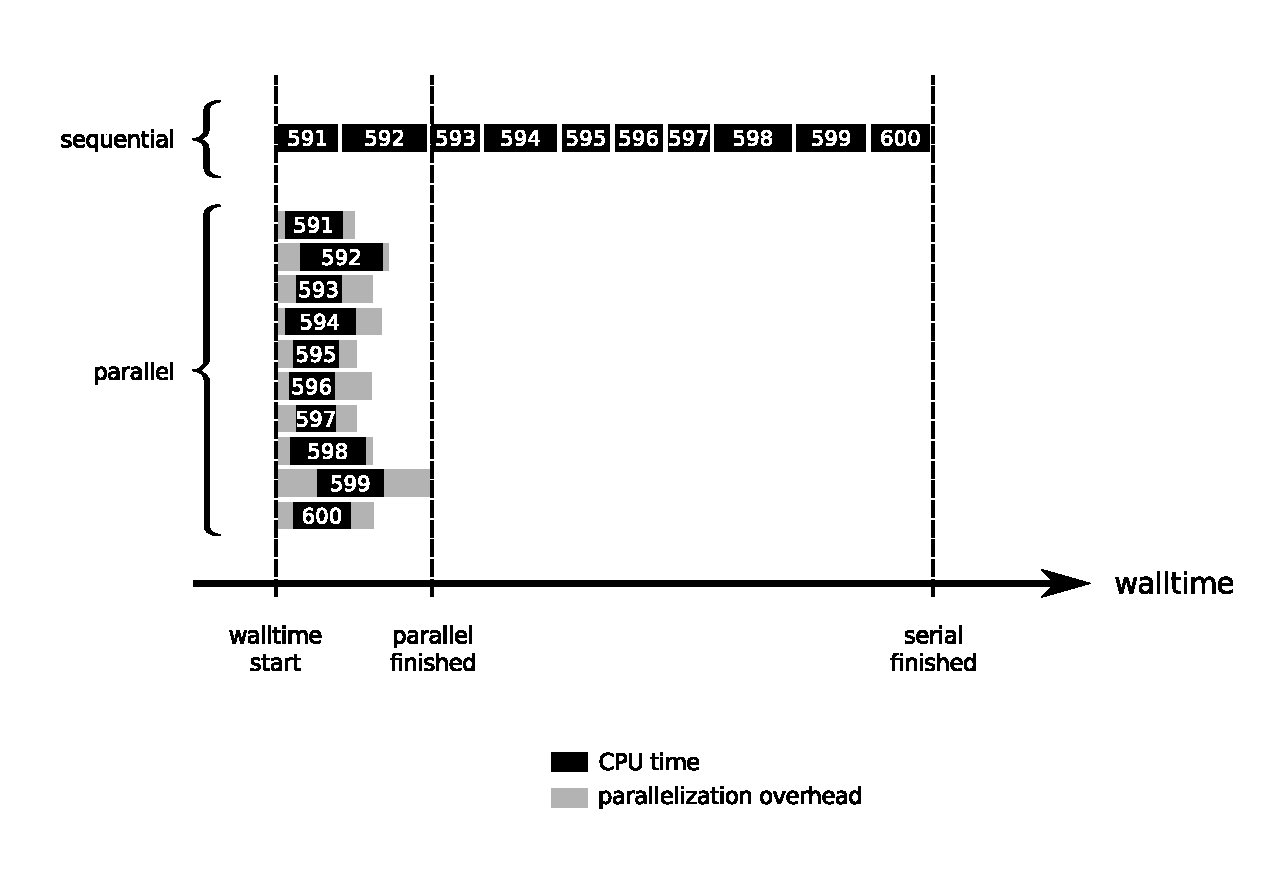
\includegraphics[width=0.9\textwidth]{./../eps/serial-parallel-walltime.eps}
  \caption{Walltime needed to complete 10 tasks 591--600 when evaluated in series or in parallel.}
  \label{fig:walltime-comparison}
\end{figure}



\section{The Master-Worker paradigm}


For Monte-Carlo type optimization, the Master-Worker paradigm\index{Master-Worker paradigm} (sometimes also referred to as Master-Slave\index{Master-Slave paradigm}) is the most common. In the Master-Worker paradigm, one of the available nodes is assigned the role of Master, while all the other nodes assume Worker roles.

\subsection{Master side}

The Master node is responsible for keeping track of the status of all Worker nodes with regard to what program a given Worker should run next, as well as to the logistics of the optimization, i.e.\,whether all nodes are connected, which nodes are busy calculating, which have finished, which are waiting for a new task, etc. Furthermore, the Master node is the brains of the optimization algorithm: the Master decides which tasks should be evaluated next. At the very beginning of the optimization, the Master typically checks whether all the nodes are online. After that, the Master will send each node all data that the Worker needs to complete its tasks. This typically includes things like the observations against which the model result will be compared, as well as the model's initial and boundary conditions---basically everything that is constant for all tasks. The Master also sends the model structure itself. Once all Workers have received the data and the model structure, the Master node determines what parameter combinations need to be sampled first. This is entirely dependent on which algorithm is used for the optimization. In any case, the Master compiles a list of all parameter combinations that need to be evaluated (i.e.\,for which the model structure needs to be run). It then distributes these parameter combinations over the available Workers, and waits for the Workers to start returning results. A result is usually in the form of an objective score or likelihood function value, but can in principle be any variable, or even a collection of variables.

\subsection{Worker side}


On the Worker side, things are pretty simple: when the Worker starts, it loads all the initial and boundary conditions that it received from the Master, after which it goes into a never-ending loop. The never-ending loop consists of just a few components: first, it waits for a new task, i.e.\,, a new parameter combination. Once it has received the parameter combination, it runs the model structure with the parameter combination it just received. After the model finishes, the Worker will typically run some sort of objective function to calculate the likelihood function value, for instance by comparing it to observations (which the Master sent to the Worker at the very beginning). The objective function's result is then sent back to the Master node, and the Worker returns to the beginning of the never-ending loop where it either continues with the next task, or waits until it receives a new one.




\begin{figure}[htb]
  \centering
    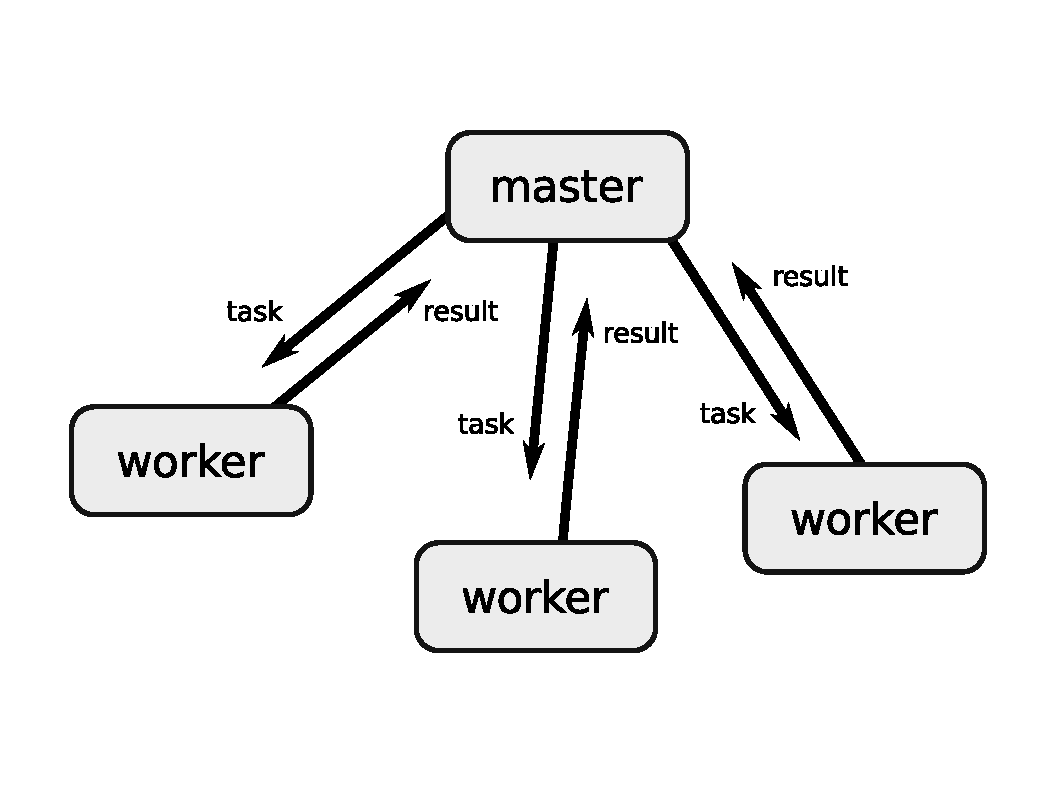
\includegraphics[width=0.9\textwidth]{./../eps/master-worker-paradigm.eps}
  \caption{Message passing between a master node and its workers.}
  \label{fig:master-worker-paradigm}
\end{figure}


%\chapter{\texttt{piped}}

In the previous chapter, I described the Master-Worker paradigm conceptually. In this chapter, we look at one specific piece of software that implements this concept. The software is called `piped'. piped\index{Linux commands!piped@\texttt{piped}} is a so-called \textit{daemon}\index{daemon}, i.e.\,a program that does not have an graphical interface but instead runs in the background\footnote{\burl{http://en.wikipedia.org/wiki/Daemon\_\%28computing\%29}}. Its task is to manage the communication between the master node and the workers (see Fig.~\ref{fig:piped}). The Master now only has to tell piped which tasks it wants to evaluate, and wait for the results while the piped program takes care of the logistics of communicating with the Worker nodes.

You can check if \lstinline[style=bashinline]{piped} is already running by checking the processes that are running system-wide:
\begin{lstlisting}[style=basic,style=bash] 
jspaaks@login4:~$ ps -ef
\end{lstlisting}
and then filter the long list of results with the \lstinline[style=bashinline]{grep} program:
\begin{lstlisting}[style=basic,style=bash]
jspaaks@login4:~$ ps -ef|grep ruby
jspaaks  17312 17193  0 00:14 pts/5    00:00:00 ruby1.9.1 ./piped.rb
jspaaks  17363 17193  0 00:14 pts/5    00:00:00 grep ruby
jspaaks@login4:~$ 
\end{lstlisting}\index{Linux commands!ps@\texttt{ps}}\index{Linux commands!grep@\texttt{grep}}

If there is an old \lstinline[style=bashinline]{piped} still running, you must terminate it using the \lstinline[style=bashinline]{kill} command followed by the identifier of the process, e.g.
\begin{lstlisting}[style=basic,style=bash]
jspaaks@login4:~$ kill 17312
\end{lstlisting}\index{Linux commands!kill@\texttt{kill}}
otherwise the messages from different \lstinline[style=bashinline]{piped} instances will get intermixed.

\begin{figure}[htb]
  \centering
    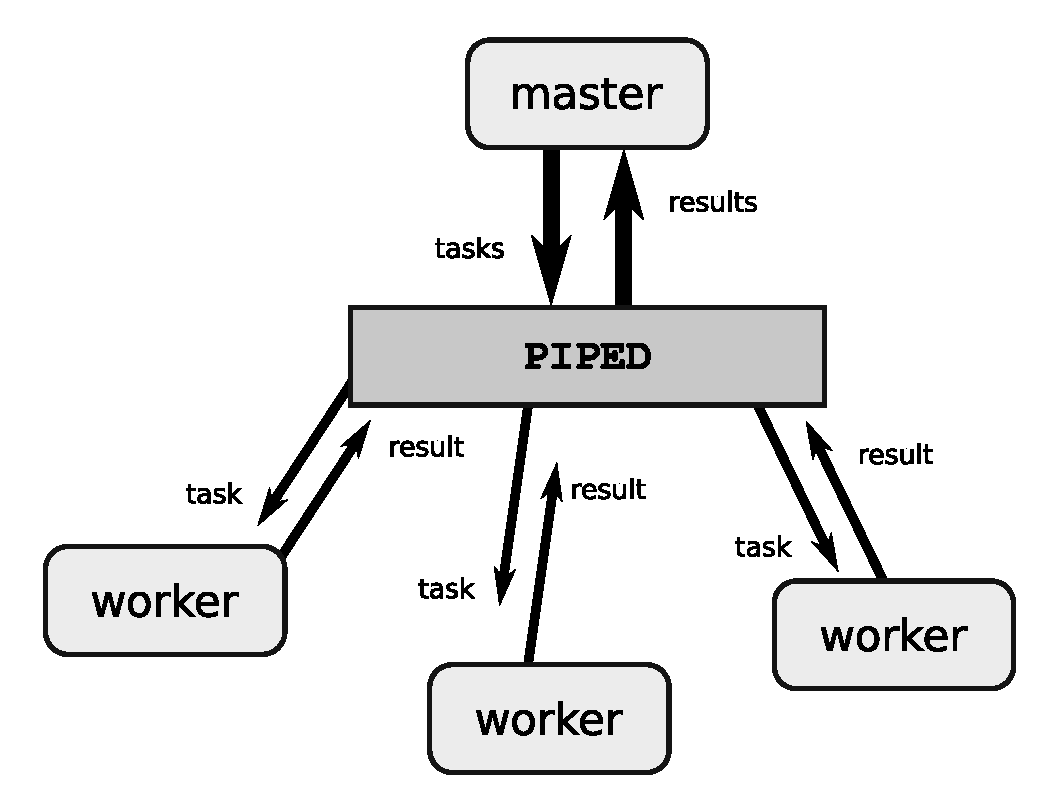
\includegraphics[width=0.9\textwidth]{./../eps/piped.eps}
  \caption{Message passing between a master node and its workers.}
  \label{fig:piped}
\end{figure}



Besides piped, there are various other softwares that implement the Master-Worker paradigm. The most commonly used Master-Worker software is probably MPI\index{Message Passing Interface}\index{MPI}, which stands for \textit{Message Passing Interface}. 

\chapter{The MMSODA Toolbox for MATLAB}
\label{ch:mmsoda}

There are various softwares that implement the Master-Worker paradigm. The most commonly used Master-Worker software is probably MPI\index{Message Passing Interface}\index{MPI}, which stands for \textit{Message Passing Interface}. Most cluster computers have some form of MPI installed. We will use the GNU version of OpenMPI\index{MPI!OpenMPI/GNU}\index{OpenMPI/GNU}, since this is the default MPI package at the LISA cluster computer.

We have developed a parallel MATLAB version of SODA \citep[e.g.][]{vrug-diks-gupt-bout-vers-2005} that makes use of MPI. The software package is called `The MMSODA Toolbox for MATLAB', or MMSODA for short (MMSODA stands for MATLAB-MPI-SODA). In this chapter, we will look at how to set it up.

MMSODA offers the functionality of a number of previously separate softwares, namely SCEM-UA \citep{vrug-gupt-bout-soro-2003}, SODA \citep{vrug-diks-gupt-bout-vers-2005,vrug-robi-vess-2005,clar-vrug-2006}, MOSCEM-UA \citep{vrug-gupt-bast-bout-soro-2003}, multi-objective SODA \citep{vrug-stau-wohl-robi-vess-2008}, the MPITB-parallel version of SCEM-UA implemented in Octave \citep{vrug-onua-robi-bout-dekk-sloo-2006}, and the MPITB-parallel version of SODA implemented in Octave \citep{vrug-gupt-onua-bout-2006}. Additionally, MMSODA offers a parallel version of multi-objective SCEM-UA, and a parallel version of multi-objective SODA, both of which did not exist previously. Moreover, MMSODA does not use Octave when running in parallel, because Octave does not evaluate code as quickly as does MATLAB. MMSODA circumvents (in a legal fashion) the license requirements that are often an impediment to parallel computation by compiling the MATLAB code into a binary which can be run without any license. Compiling the binary, however, does require a license, both for the MATLAB program itself, as well as for the MATLAB Compiler Runtime Toolbox. Fortunately, the required licenses are available on most cluster environments targeting a scientific and engineering audience.

In short, the acronyms mentioned above mean that: MMSODA can do parameter tuning with or without intermediate state updating by an ensemble Kalman Filter; that MMSODA supports both single-objective and multi-objective optimization; and that the optimization can be run either sequentially on a local machine, or in parallel on a cluster computer.

The serial/parallel capability is particularly attractive, since it allows the users to set up their optimizations locally on their own machines, thus ensuring a familiar development environment without the need to make the code compatible with Octave syntax. When the user finishes setting up the optimization, running it on a cluster computer is simply a matter of copying the relevant directory to the cluster storage using standard tools (e.g. WinSCP) and compiling the software by executing a script that comes with the software. Furthermore, MMSODA is fully documented with HTML documentation which can be accessed in the same way as MATLAB's built-in commands, namely through the \texttt{doc} command.

The remainder of this chapter explains how to set up increasingly sophisticated optimizations within the MMSODA framework. Let's start off with a single-objective SCEM-UA optimization of a benchmark function \texttt{calcLikelihood()}, and let's not do anything in parallel just yet.

\section{MMSODA in `bypass' mode; sequential execution}

\smallq{In your file explorer program, navigate to the directory where you unzipped the file from \burl{https://github.com/NLeSC/esibayes}.}

As you can see, the `esibayes-master' directory contains a number of subdirectories. Among these, the `src/mmsoda-toolbox' and `examples' subdirectories are probably the most important: the former contains the MATLAB toolbox that this chapter is about, while the latter contains a couple of examples of how to use the MMSODA toolbox for MATLAB with different models and different configurations. There are a few other directories, such as `manual', `testing' and `code-quality-metrics'. The `manual' directory contains all the files pertaining to the document you have before you. The `testing' and `code-quality-metrics' directories are part of the software quality control process: whenever we change something in MMSODA's code, a number of tests from the `testing' directory are run automatically. The test results are subsequently posted in `code-quality-metrics'. With this so-called unit-testing, we can verify that updates to one part of the algorithm do not accidentally break other parts.

\smallq{Let's get started by making a new directory that will hold all of our MMSODA projects. Let's call this directory `mmsoda-projects' (you can put this directory anywhere you have write access on your system). Change directory into `mmsoda-projects', create a subdirectory `example1', with three subdirectories in it called `data', `model', and `results'. (We won't always use all three directories, but MMSODA expects all three to be present regardless of whether they are used). So now you have a directory somewhere on your local storage device that has at least the following subdirectories:
\begin{itemize}
\item{mmsoda-projects/example1}
\item{mmsoda-projects/example1/data}
\item{mmsoda-projects/example1/model}
\item{mmsoda-projects/example1/results}
\end{itemize}
}

\smallq{Open MATLAB and set your working directory to `example1'.}

\smallq{Before we can use the functionality provided by the MMSODA Toolbox for MATLAB, we need to tell MATLAB about its existence by adding the main directory to the MATLAB search path. You must do this using the \texttt{addpath} command as follows:\\
\texttt{>> addpath(\squote{s})}, in which \texttt{s} indicates the location of the MMSODA directory. For example, it could be:\\
\texttt{>> addpath(\squote{C:\textbackslash{}Users\textbackslash{}jspaaks\textbackslash{}esibayes-master\textbackslash{}src\textbackslash{}mmsoda-toolbox})}\\ on a Windows machine or \\
\texttt{>> addpath(\squote{/home/jspaaks/esibayes-master/src/mmsoda-toolbox})}\\
on Linux.
}
\smallq{At the MATLAB prompt, type:\\
\texttt{>> mmsoda --docinstall}\\
to complete the MMSODA setup. In principle, you only have to run this command once per MATLAB session, as long as you do not change the location of the `mmsoda-toolbox' directory on your storage.}

\smallq{Test whether everything works as it should by typing: \\
\texttt{>> doc mmsoda} \\
at the MATLAB command prompt. This should bring up MATLAB's help browser. Click on the link `View HTML documentation for this function in the help browser'. You should now see an overview of the functions comprising the MMSODA Toolbox for MATLAB.}

\smallq{Spend at least 12 minutes to browse through the documentation. In any case, make sure to read the documentation on `mmsoda.m'.}

The function that we want to maximize implements the double-normal probability distribution:
\begin{equation}\label{eq:double-normal}
\begin{align}
p = \frac{1}{2}\cdot{}\frac{1}{\sqrt{2\pi\sigma_1^2}}\:e^\mathlarger{-\frac{1}{2}\left(\frac{x-\mu_1}{\sigma_1}\right)^2} & +\dots \\
    \frac{1}{2}\cdot{}\frac{1}{\sqrt{2\pi\sigma_2^2}}\:e^\mathlarger{-\frac{1}{2}\left(\frac{x-\mu_2}{\sigma_2}\right)^2} & \\
\end{align}
\end{equation}
with $\mu_1 = -10$, $\sigma_1 = 3$, $\mu_2 = 5$, $\sigma_2 = 1$, respectively. The parameter that is optimized (or, equivalently, whose probability distribution we will estimate by means of the MMSODA Toolbox for MATLAB) is $x$. For example, for $x=4.5$, $p = 0.1760$.

%p=\frac{1}{2}\cdot{}\frac{1}{\sqrt{2\cdot{}\pi\cdot{}\sigma{}_1}}\cdot{}\mathrm{exp}\left[-\frac{1}{2}\cdot{}\left(\frac{x-\mu_1}{\sigma_1} \right)^2 \right] \quad & + \\
%\frac{1}{2}\cdot{}\frac{1}{\sqrt{2\cdot{}\pi\cdot{}\sigma{}_2}}\cdot{}\mathrm{exp}\left[-\frac{1}{2}\cdot{}\left(\frac{x-\mu_2}{\sigma_2} \right)^2 \right] \quad & \\

Because MMSODA expects the objective function to return a log-likelihood $l$, we must actually take the natural logarithm of $p$ as the objective score:
\begin{equation}\label{eq:log-likelihood}
l=\mathrm{ln}\left(p\right)
\end{equation}

\subsection{Creating the `constants.mat' and `conf.mat' files}

Before we actually start writing any code for this objective function however, let's first create the `conf.mat'\index{conf.mat} and `constants.mat'\index{constants.mat} files that are always needed for running \texttt{mmsoda()}.

\smallq{Start a new text file in the MATLAB editor and save it as `makeconf.m'\index{makeconf.m} in the current working directory (`mmsoda-projects/example1').}

\smallq{At the first line in `makeconf.m', add the following:\\
\texttt{function makeconf()}\\}

Now we need to edit the contents of `makeconf.m' as follows.

\smallq{At the MATLAB prompt, type \\
\texttt{doc mmsoda} \\
and bring up the HTML documentation for the \texttt{mmsoda()} function.}

Near the bottom of the documentation, there is an overview of the configuration variables that must be specified for a given type of optimization. For our double-normal example, we will use MMSODA in `bypass' mode\index{MMSODA!bypass mode}. This mode is used when the log-likelihood can be estimated directly from the parameter vector, without the need to run a (dynamic) model structure.

\smallq{If you look in the table with the configuration variables, you'll see that only 5 variables are required for running MMSODA in `bypass' mode. These are \texttt{modeStr}, \texttt{objCallStr}, \texttt{parNames}, \texttt{parSpaceHiBound}, and \texttt{parSpaceLoBound}. Make sure you understand the description for each of these.}

\smallq{Return to `makeconf.m' and add the following:\\
\texttt{modeStr = \squote{bypass};}\\
\texttt{objCallStr = \squote{calcLikelihood};}\\
\texttt{parNames = \{\squote{x}\};}\\
\texttt{parSpaceHiBound = [10];}\\
\texttt{parSpaceLoBound = [-30];}\\
}

With the above settings we specify that we want MMSODA to do a bypass run, in which the function `calcLikelihood.m' (which we will create shortly) is optimized. \texttt{calcLikelihood} has one tunable parameter, \texttt{x}. The bounds that we set on the search for the optimal value of \texttt{x} are \texttt{[-30,10]}.

\smallq{At the last line in `makeconf.m', add the following:\\
\texttt{save(\squote{./results/conf.mat})}\\}

\smallq{Save and close `makeconf.m'.}

Next, we need to create `constants.mat' by a similar procedure.

\smallq{Create a new m-file in the current working directory called `makeconstants.m'.\index{makeconstants.m}}

\smallq{At the first line in `makeconstants.m', type:\\
\texttt{function makeconstants()}}

Now we need to assign the constants, i.e.\,the variables that \texttt{calcLikelihood} needs in order to calculate the log-likelihood according to equations~\ref{eq:double-normal}--\ref{eq:log-likelihood}.

\smallq{In `makeconstants.m', add:\\
\texttt{parMu1 = -10;}\\
\texttt{parSigma1 = 3;}\\
\texttt{parMu2 = 5;}\\
\texttt{parSigma2 = 1;}\\
i.e. the two means and two standard deviations for the double normal distribution.
}

\smallq{At the last line in `makeconstants.m', add\\
\texttt{save(\squote{./data/constants.mat})}
}

\smallq{Save and close `makeconstants.m'.}

Finally, we need to create the objective function m-file that implements equations~\ref{eq:double-normal} and \ref{eq:log-likelihood}.

\subsection{Creating the objective function m-file}

\smallq{Create a new m-file, called `calcLikelihood.m' and save it in the subdirectory `./model'.}

\smallq{Open `./model/calcLikelihood.m'. MMSODA uses a standardized way of passing the input and output arguments to and from the objective function, so the first line is always exactly the same (with the exception of the name of the function \texttt{calcLikelihood}, which may vary), like so:\\
\texttt{function objScore = calcLikelihood(conf,constants,modelOutput,parVec)}
}

\smallq{As a second line, type: \\
\texttt{mmsodaUnpack()}\index{MMSODA functions!mmsodaUnpack@\texttt{mmsodaUnpack}}\\
\texttt{mmsodaUnpack} uses the information from the input arguments to construct the variable \texttt{x} and to assign it a value based on the value of \texttt{parVec}. Similarly, it uses information from the \texttt{constants} variable to construct the model constants and to assign them the correct values.}

Now that we have \texttt{parMu1}, \texttt{parSigma1}, \texttt{parMu2}, \texttt{parSigma2}, and \texttt{x} we can calculate the probability density \texttt{dens} as follows:
\begin{verbatim}
dens = (1/(sqrt(2*pi*parSigma1^2))*exp(-(1/2)*((x-parMu1)/parSigma1)^2) + ...
        1/(sqrt(2*pi*parSigma2^2))*exp(-(1/2)*((x-parMu2)/parSigma2)^2))/2;
\end{verbatim}

\smallq{Add this calculation to your \texttt{calcLikelihood} function.}

\smallq{Don't forget that MMSODA expects a log-likelihood however, so as a final line in \texttt{calcLikelihood}, add:\\
\texttt{objScore = log(dens);}}

\smallq{Save and close `calcLikelihood.m'.}

\subsection{Running the optimization locally}

\smallq{Make sure that the current working directory is the `example1' directory. At the MATLAB command prompt, type:\\
\texttt{>> makeconf()}\\
and check that a new file `conf.mat' is created in subdirectory `./results'.}

\smallq{At the MATLAB command prompt, type:\\
\texttt{>> makeconstants()}\\
and check that a new file `constants.mat' is created in subdirectory `./data'.}

\smallq{At the command prompt, type \texttt{clear} to clear the workspace if there are any variables in it.}

\smallq{Now, we are ready to run the optimization. At the MATLAB command prompt, type:\\
\texttt{>> [evalResults,critGelRub,sequences,metropolisRejects,conf] = mmsoda();}\\
and wait for the optimization to finish. Input arguments to \texttt{mmsoda}\index{MMSODA functions!mmsoda@\texttt{mmsoda}} are not required, since \texttt{mmsoda} knows to look in `./results/conf.mat' for the configuration, in `./data/constants.mat' for the model constants, and in `./model' for the model functions and objective functions.}

\subsection{Interpreting the results}

Once the optimization finishes, you should have 5 variables in your workspace: \texttt{evalResults}, \texttt{critGelRub}, \texttt{sequences}, \texttt{metropolisRejects}, and \texttt{conf}. Refer to the \texttt{mmsoda()} documentation for a description of what these variables are and how they are laid out.

Let's explore the results by making a histogram of the occurence of certain parameter values. You could simply use MATLAB's built-in \texttt{hist()} function to do this, but it is often more convient to use a specialized function that comes pre-packaged with MMSODA like so:\\
\texttt{ >> mmsodaSubplotScreen(2,2,1);}\index{MMSODA functions!mmsodaSubplotScreen@\texttt{mmsodaSubplotScreen}}\\
\texttt{ >> mmsodaMargHist(conf,evalResults);}\index{MMSODA functions!mmsodaMargHist@\texttt{mmsodaMargHist}}\\

\smallq{Refer to the documentation of these two functions to see how they work and use the optional \texttt{\squote{nHistory}} argument to show the marginal histogram based on the last quarter of the \texttt{evalResults} record. Your result should look like Fig.~\ref{fig:mmsodaMargHist}.}


\begin{figure}[htb]
  \centering
    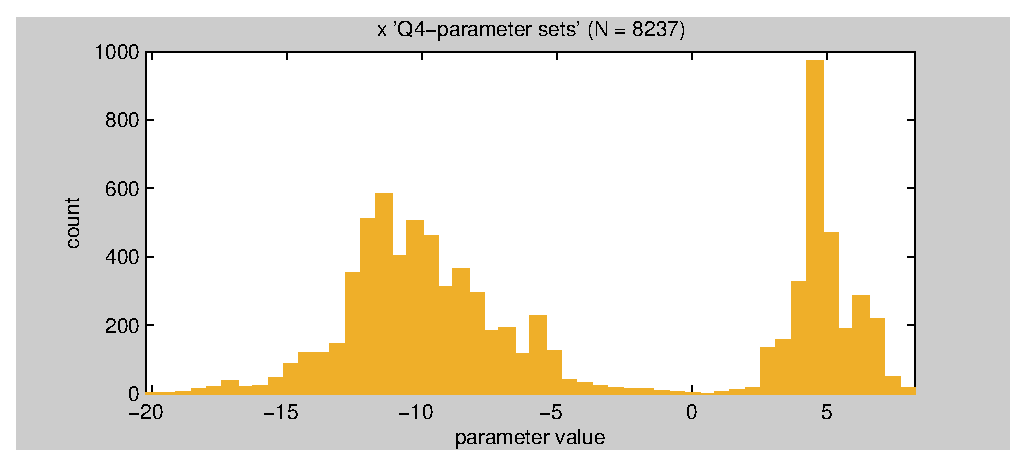
\includegraphics[width=\linewidth , keepaspectratio]{./../eps/mmsodaMargHist.eps}
  \caption{Histogram for the Q4 parameter sets for the double-normal model.}
  \label{fig:mmsodaMargHist}
\end{figure}


\smallq{Refer to the documentation on how to use \texttt{mmsodaPlotSeq}\index{MMSODA functions!mmsodaPlotSeq@\texttt{mmsodaPlotSeq}}. Create another figure on the right side of your screen, in which you visualize the record of sequences. Use the \texttt{\squote{showRejects}} option to hide the samples that were rejected as part of the Metropolis scheme. Your result should look like Fig.~\ref{fig:mmsodaPlotSeq}.}


\begin{figure}[htb]
  \centering
    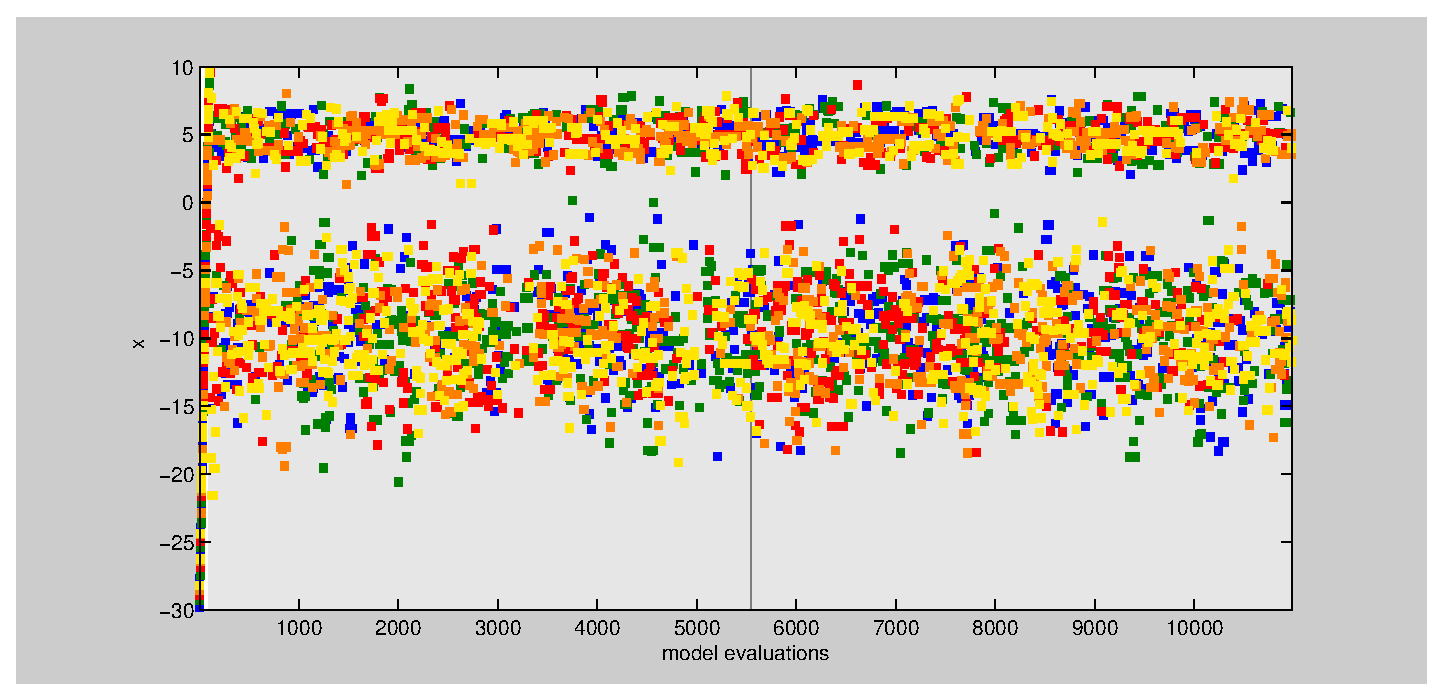
\includegraphics[width=\linewidth , keepaspectratio]{./../eps/mmsodaPlotSeq.eps}
  \caption{History of samples taken from the 1-D parameter space by \mbox{SCEM-UA} during optimization of the double-normal model.}
  \label{fig:mmsodaPlotSeq}
\end{figure}

\smallq{Refer back to the documentation on the \texttt{mmsoda} function; specifically, browse through some of the configuration options for running MMSODA in `bypass' mode. Alter your `makeconf.m' with the options that you find useful, and re-run the optimization.}

\smallq{When you are satisfied with the way you set up MMSODA locally, you can make preparations for running it in parallel on the LISA cluster computer. Running on LISA requires a so-called `Makefile'\index{Makefile} as well as a jobscript\index{jobscript}, both of which are tricky to write yourself. Therefore, the MMSODA Toolbox for MATLAB comes with a function that helps you generate the correct files by asking a series of questions. At the MATLAB prompt, type:\\
\texttt{>> mmsodaPrepParallelFiles(\squote{s})}\index{MMSODA functions!mmsodaPrepParallelFiles@\texttt{mmsodaPrepParallelFiles}} \\
but substitute \texttt{s} with the location of the MMSODA Toolbox for MATLAB as used on the LISA cluster. So for me, it would be:\\
\texttt{>> mmsodaPrepParallelFiles(\squote{/home/jspaaks/esibayes-master/src/mmsoda-toolbox}}) \\
Now use the following information to answer \texttt{mmsodaPrepParallelFiles}'s questions:\\
\begin{enumerate}\label{li:answers-mmsodaPrepParallelFiles}
\item{the optimization will run on one of the login nodes;}
\item{we want not much verbal feedback from the program;}
\item{we don't want to use all the cores on the login node;}
\item{we want to start 4 processes;}
\item{we don't want to save the timing information.}
\end{enumerate}\\
(Note that \texttt{mmsodaPrepParallelFiles()} indicates the default answer with brackets, and that you can accept the default by simply pressing Enter.)
}

When \texttt{mmsodaPrepParallelFiles()} finishes, it prints a message in the command window that tells you what file it has just created. This file should be located in the current working directory. We will use it shortly to start the optimization on the cluster. You can take a look a its contents in Notepad or a similar program, but make sure not to change anything. Besides the jobscript, there should also be a new file called `Makefile'. Just like the jobscript, this is also a plain text file, so you can view its contents in Notepad as well. Again, make sure not to accidentally change anything.


\section{MMSODA in `bypass' mode; parallel execution}

\smallq{Use WinSCP or the alternative program of your choice to copy the `example1' and `mmsoda' directories, including all of their contents, to your storage on the cluster, i.e.\,anywhere under the `/home/$<$username$>$/' directory.}

When you are satisfied with the way you set up MMSODA locally, you can run it on the LISA cluster computer. In order to do so, we must first compile the software into a so-called `binary'\index{binary} or `executable'\index{executable}. You do not need to worry about how this works in detail, it is just a matter of running the Linux \texttt{make} command. \texttt{make} looks for a file called `Makefile' that was just created by \texttt{mmsodaPrepParallelFiles()}. Based on the contents of `Makefile', \texttt{make} collects all the relevant software (your model files, your objective functions, the MMSODA code, as well as the code that enables communication between the Master and the Workers) and creates two files that are necessary to run your code within MMSODA using multiple cores.

\subsection{Compiling MMSODA and your model code into a binary}

\smallq{Use PuTTY to start an SSH connection to the LISA cluster.}

\smallq{In the PuTTY terminal, load the MATLAB program and MPI programs by typing:\\
\texttt{module load matlab}\\
This command will not give any feedback on the success or otherwise of the command, but you could check by typing the following command:\\
\texttt{module list}\\
which should now include MATLAB. Next, type\\
\texttt{module load openmpi/gnu}\\
to load the MPI software.
}

\smallq{Use the \texttt{cd} command to set `example1' as your current directory if you hadn't already done so.}

\smallq{Now we are ready to compile. At the terminal, type:\index{Linux commands!make@\texttt{make}}\\
\texttt{make}\\
You should see some text scrolling over your screen---it takes about 60 seconds or so to complete. The \texttt{make} command looks for a file called `Makefile'\index{Makefile} in the current directory, and uses the information in it to correctly build the binary `matlabprog' and the library that it needs, called `libmmpi.so'.}

\smallq{After \texttt{make} finishes, list the directory contents with \texttt{ls -l} and verify that
you now have two extra files `matlabprog' and `libmmpi.so'.}

Starting the optimization requires that we adjust the `permission bits'\index{permission bits} for the `run-mmsoda.sh'\index{run-mmsoda.sh} file that was just created by \texttt{mmsodaPrepParallelFiles()}. Permission bits indicate what a specific user is allowed to do with a particular file. (You may know the same concept from Windows, where you can sometimes have `Read-only' versions of a file). The permission bits are listed as the first 10 columns in the output from \texttt{ls -l}:

\Needspace{12\baselineskip}

\begin{lstlisting}[style=basic,style=bash]
jspaaks@login1:~/esibayes-master/example1$ ls -l
total 204
drwxr-xr-x 2 jspaaks jspaaks     26 Jan 16 16:09 data
-rwxrwxr-x 1 jspaaks jspaaks 172792 Jan 18 11:57 libmmpi.so
-rw-r--r-- 1 jspaaks jspaaks    176 Jan 16 16:02 makeconf.m
-rw-r--r-- 1 jspaaks jspaaks    120 Jan 16 15:06 makeconstants.m
-rw-rw-r-- 1 jspaaks jspaaks   1357 Jan 16 16:10 Makefile
-rwxrwxr-x 1 jspaaks jspaaks  11969 Jan 18 11:57 matlabprog
drwxr-xr-x 2 jspaaks jspaaks     29 Jan 16 16:09 model
drwxr-xr-x 2 jspaaks jspaaks   4096 Jan 16 17:36 results
-rw-r--r-- 1 jspaaks jspaaks    580 Jan 18 13:26 run-mmsoda.sh
jspaaks@login1:~/esibayes-master/example1$
\end{lstlisting}

For `run-mmsoda.sh'\index{run-mmsoda.sh}, the permissions are set to \texttt{-rw-r--r--}. The first character \texttt{-} indicates that `run-mmsoda.sh' is a file (as opposed to a \texttt{d} which would indicate a directory). Characters 2, 3 and 4 (\texttt{rw-}) indicate what you, the currently logged-in user, is allowed to do with `run-mmsoda.sh'. Currently, you are allowed to read from (\texttt{r}) and write to (\texttt{w}) `run-mmsoda.sh'. The \texttt{-} character from the fourth column of \texttt{ls -l} indicates that you are currently not allowed to execute `run-mmsoda.sh' as a script.

\smallq{Change the permission bit for `run-mmsoda.sh' by typing at the prompt:\index{Linux commands!chmod@\texttt{chmod}}\\
\texttt{chmod u+x run-mmsoda.sh}\\
In normal English, this command translates to ``\texttt{Ch}ange the \texttt{mod}e of file `run-mmsoda.sh' by adding (\texttt{+}) the executable permission (\texttt{x}) for the current user (\texttt{u})''. Check that the permissions have changed to \texttt{-rwxr--r--}.}

\smallq{Now we are ready to start the optimization in parallel on the login node. At the beginning of the optimization, you will see a lot of text scrolling over your terminal screen which at this stage probably does not make much sense. Don't worry if you don't understand it---we will look at it in greater detail later. Eventually, you'll get messages along the lines of `Evaluating parameter sets 1-100', `Evaluating parameter sets 101-120', etc. Start the optimization by typing at the terminal:\\
\texttt{./run-mmsoda.sh}\\
(Don't omit the \texttt{./} at the beginning, otherwise it won't work.)
}

%\smallq{\textit{Parallel execution is actually slower than in series due to Amdahl's Law and due to the presence of other users on the login nodes.}\index{todo}}

\smallq{After the optimization finishes, the results need to be transferred to your local system. Copy the contents of `example1/results/' from the remote system to `example1/results/' on your local machine (you can overwrite the old files in `example1/results/' on your local machine if you want).
}

\smallq{On your local machine, clear the workspace, and load MMSODA's output variables using:\\
\texttt{ >> load(\squote{./results/bypass-so-results.mat})}\\
You can now use any of the MMSODA visualizations (or MATLAB visualizations for that matter), in just the same way as if the results had been calculated locally.}


\smallq{Now that you know what information goes where for MMSODA in `bypass' mode, it may be useful to review some of the other examples in the `esibayes-master' directory. On your local machine, explore the configurations for a few of the other `bypass' mode directories. Try running MMSODA for those configurations, but make sure MATLAB is set to the correct working directory when \texttt{mmsoda} is started.}


% % % % % % % % % % % % % % % % % % % % % % % % % % % % % % % % % %

\section{MMSODA in `scemua' mode; sequential execution}

Now that we have a working example of MMSODA in `bypass' mode, let's try our hand at something a little more difficult: optimizing the parameters of a dynamic model\index{MMSODA!scemua mode}. This works in more or less the same way as the bypass mode, except that the likelihood is determined by comparing a model prediction to observations, while taking into account the uncertainty of the latter. Let's first make a small digression and look at the general structure of dynamic models. Such models simulate the behavior of a number of states over time. As an example, Fig.~\ref{fig:states-and-flows} shows a system in which there are two states. The first state is the water level in a tank which has a small hole in the bottom. The second state is the water level in a tank that has no leaks. The first tank discharges into the second. The rate of discharge $Q$ is dependent on the volume of water in the tank $V_{tank_1}$ and on a resistance parameter $R$ (if there is a big leak in the first tank, the resistance is low, but if the leak is only small, the resistance is high). The model simulates discharge as follows:
\begin{equation}\label{eq:flow-from-tank1}
Q = \frac{V_{tank_1}}{-R}
\end{equation}

Given the state of the upper tank at a given point in time $V_{tank_1}(t)$, Eq.\,\ref{eq:flow-from-tank1} may be used to calculate the corresponding flow at time $t$. Furthermore, the current state $V_{tank_1}(t)$ and flow $Q(t)$ may be used to simulate the state at a later time, $t+\Delta{}t_{sim}$, provided that $\Delta{}t_{sim}$ is sufficiently small:
\begin{equation}\label{eq:numerical-integration-tank1}
V_{tank_1}(t+\Delta{}t_{sim}) = V_{tank_1}(t) + Q(t)*\Delta{}t_{sim}
\end{equation}
\begin{equation}\label{eq:numerical-integration-tank2}
V_{tank_2}(t+\Delta{}t_{sim}) = V_{tank_2}(t) - Q(t)*\Delta{}t_{sim}
\end{equation}

If the initial state of the system $V_{tank_1}(t_0)$ and $V_{tank_2}(t_0)$ is known, and if the resistance parameter $R$ has been assigned, repeated application of Eqs.\,\ref{eq:flow-from-tank1}--\ref{eq:numerical-integration-tank2} thus enables constructing a time series of simulated values for $V_{tank_1}$ and $V_{tank_2}$.

\begin{figure}[htb]
  \centering
    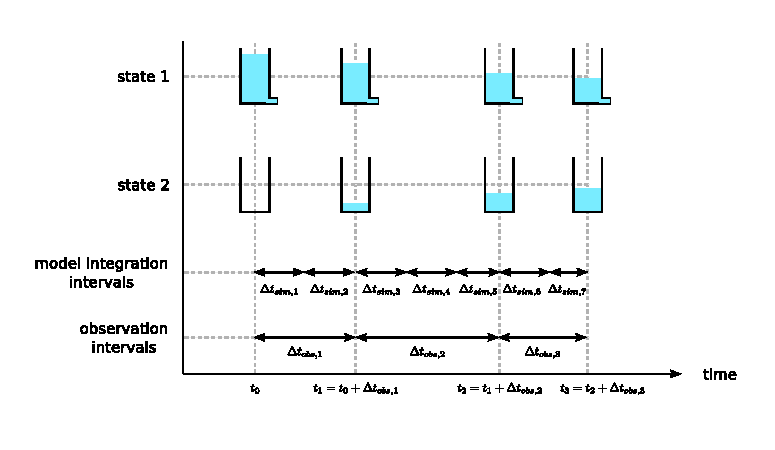
\includegraphics[width=\linewidth,keepaspectratio]{./../eps/states-and-flows.eps}
  \caption{The general structure of dynamic models.}
  \label{fig:states-and-flows}
\end{figure}

It is quite common that not all the parameter values are known beforehand, so in order to make predictions with the model, it becomes necessary to estimate the model parameter values by comparing simulation results to observations of the system's states. The model must therefore be set up such that it returns the system's state at the times for which an observation is available, otherwise the comparison isn't much use. Since the time interval between observations $\Delta{}t_{obs}$ can be (much) larger than the model integration interval $\Delta{}t_{sim}$, multiple model integration steps are often needed in between observation times. Listing~\ref{list:lintank-script} shows a simple MATLAB script that implements the system depicted in Figure~\ref{fig:states-and-flows}.  A copy of the script has been included as `other/lintank\_script.m'.

\Needspace{7\baselineskip}

Over the next few exercises, we will:
\begin{enumerate}
\item{prepare a `constants.mat',}
\item{prepare a `conf.mat',}
\item{prepare the main model m-file by adapting `lintank\_script.m' such that it can be used within the MMSODA framework,}
\item{construct a likelihood function.}
\end{enumerate}
%The above four steps are necessary for all types of optimization except `bypass'.


\smallq{Before we start, make sure you understand how the `lintank\_script.m' works by studying Listing~\ref{list:lintank-script} and running through it line-by-line using MATLAB's debugging capabilities.}

\Needspace{64\baselineskip}
\lstinputlisting[style=basic,style=matlab,style=numbered,style=spacious,caption={Simple MATLAB script that implements the system depicted in Figure~\ref{fig:states-and-flows}. A copy of this script has been included as `other/lintank\_script.m'.},label=list:lintank-script]{./../m/lintank_script.m}

\begin{figure}[htb]
  \centering
    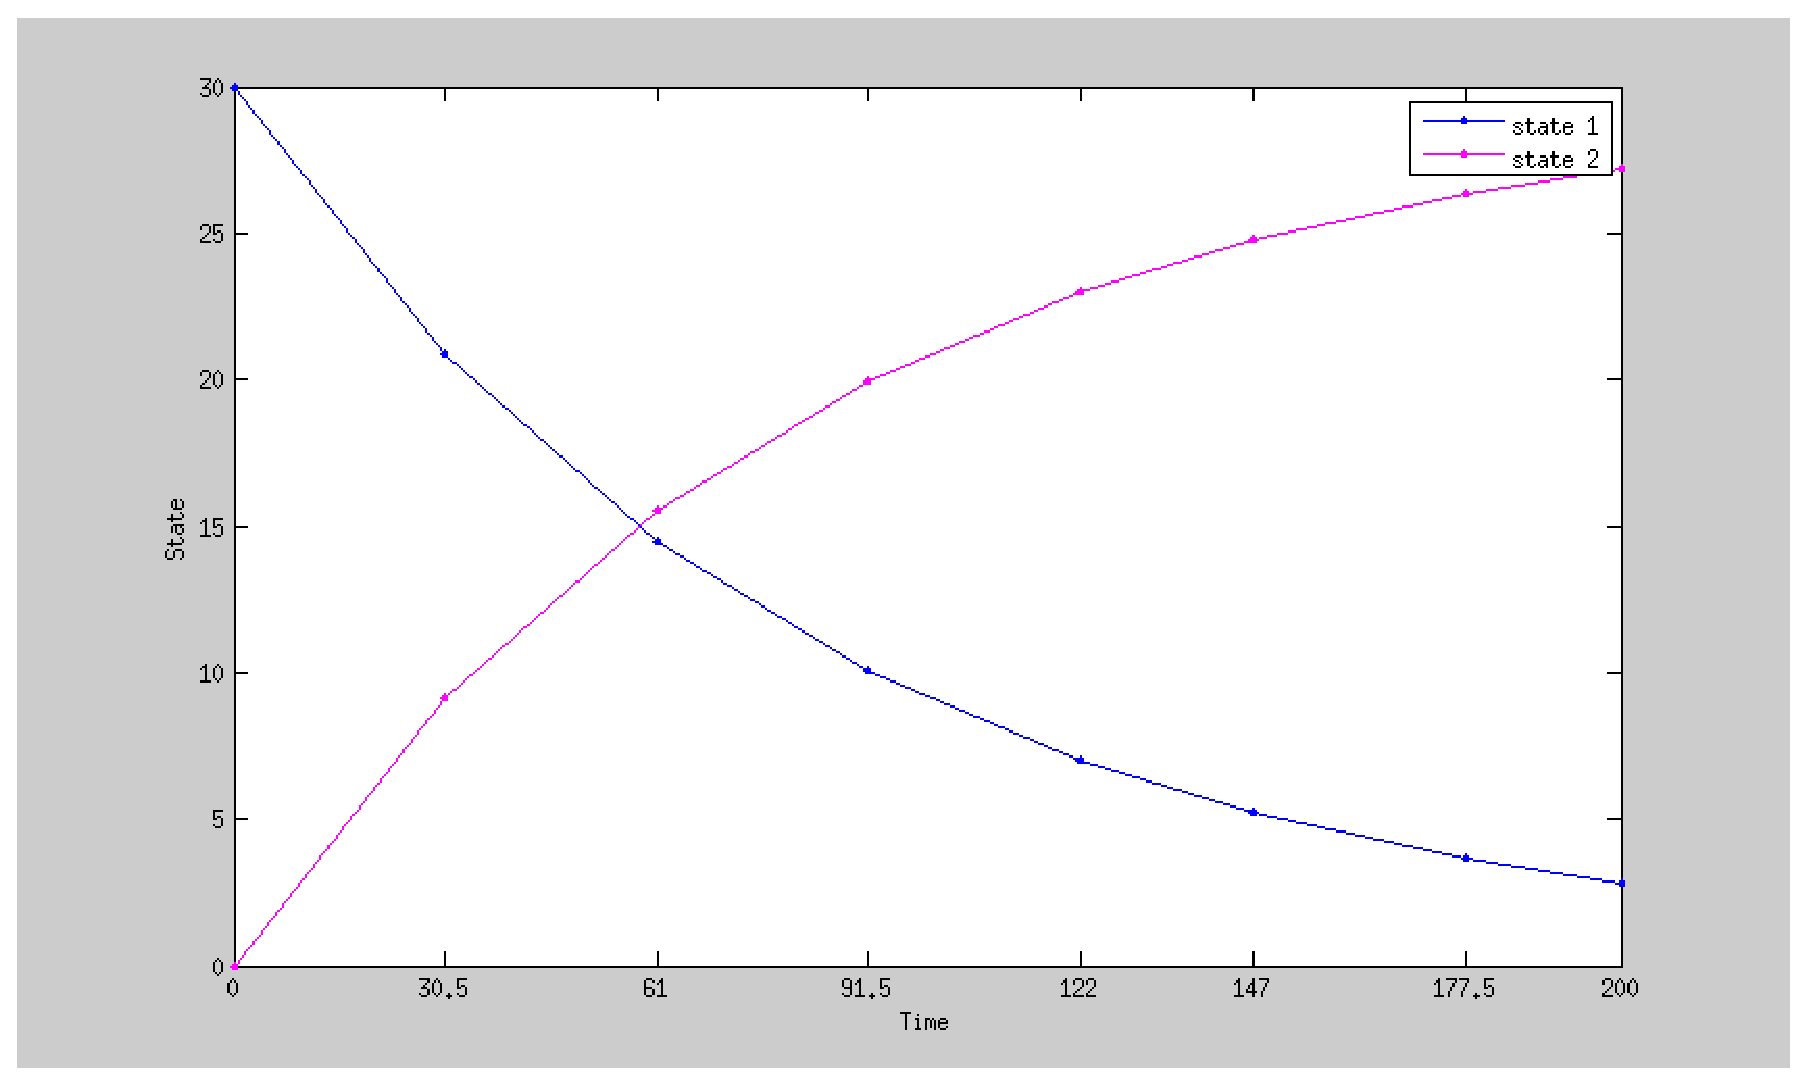
\includegraphics[width=\linewidth,keepaspectratio]{./../eps/result-of-lintank-script.eps}
  \caption{Result of running the code from Listing~\ref{list:lintank-script}.}
  \label{fig:result-of-lintank-script}
\end{figure}


\smallq{Create a new directory structure with the required subdirectories just like you did before. Call the top directory `example2'. Verify that the `example2' directory is at the same level as the `mmsoda-toolbox' directory.}

\smallq{Read the MMSODA documentation on `the dynamic model' (see Figure~\ref{fig:doc-the-dynamic-model}).}

\begin{figure}[htb]
  \centering
    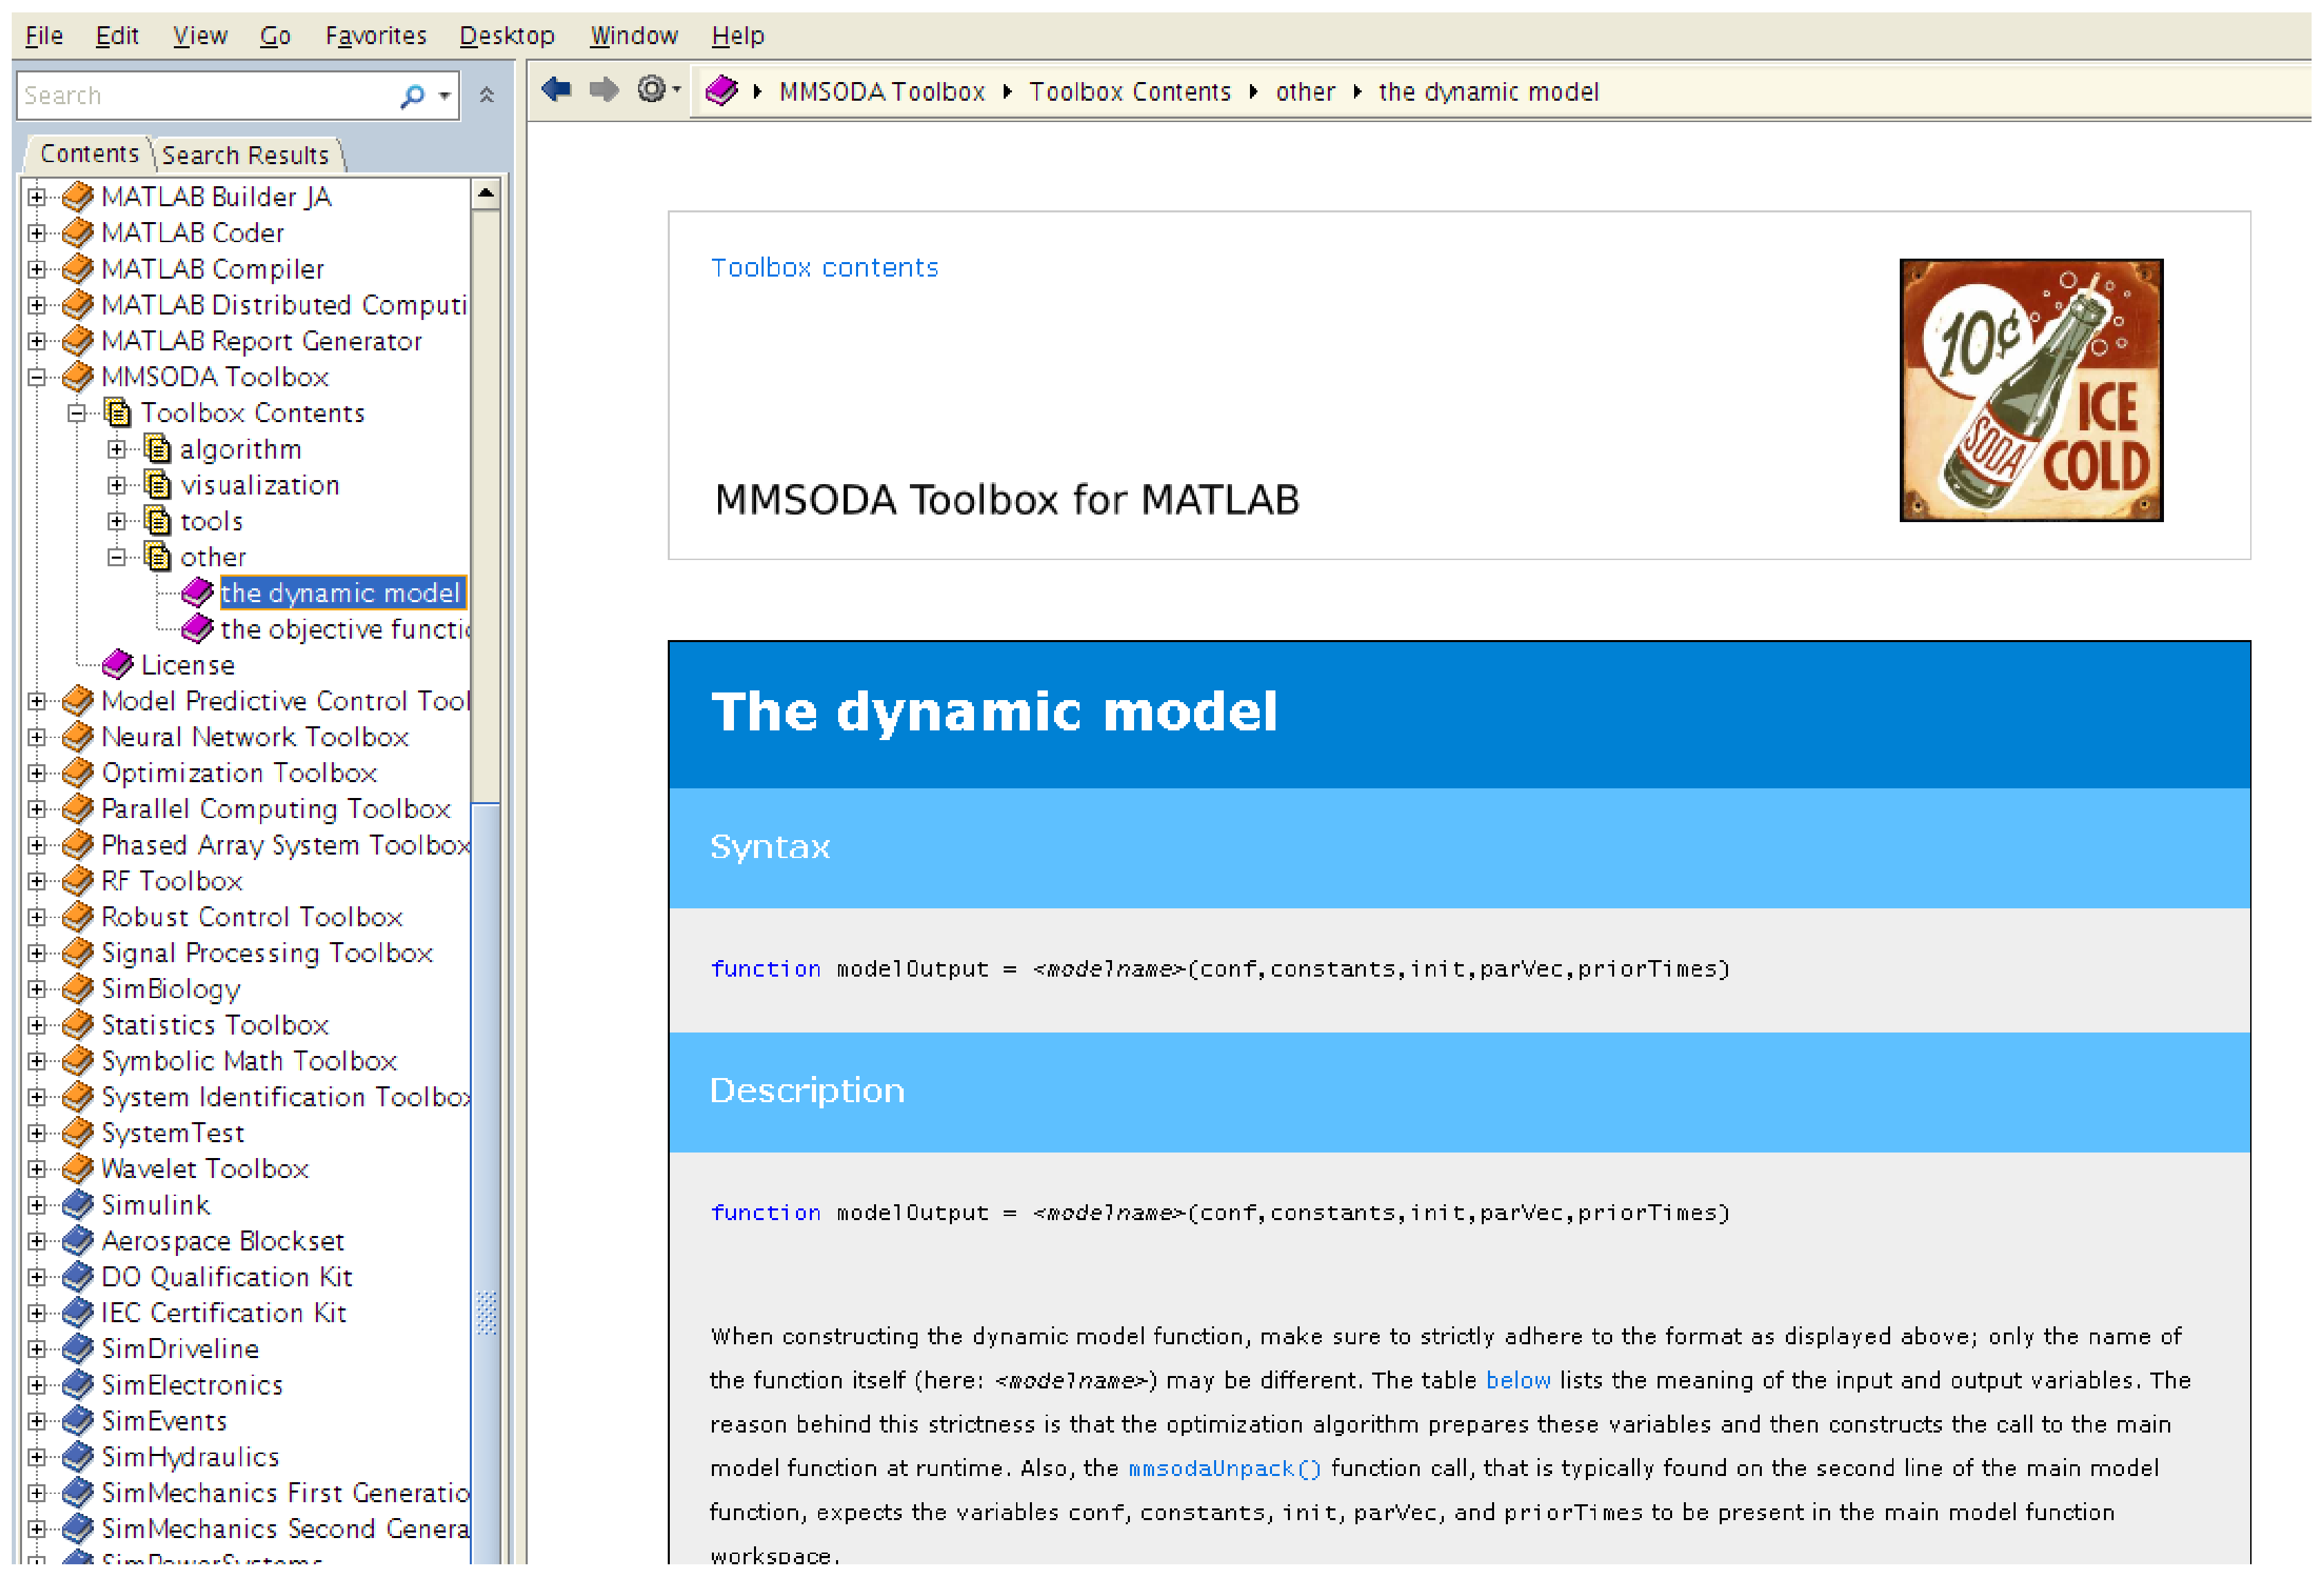
\includegraphics[width=\linewidth,keepaspectratio]{./../eps/doc-the-dynamic-model.eps}
  \caption{MATLAB documentation on how to set up the dynamic model.}
  \label{fig:doc-the-dynamic-model}
\end{figure}

In the initialization part of Listing~\ref{list:lintank-script}, 10 variables (\texttt{R}, \texttt{state1Init}, \texttt{state2Init}, \texttt{priorTimes}, \texttt{tNow}, \texttt{tEnd}, \texttt{dtSimDefault}, \texttt{rec}, \texttt{state1}, and \texttt{state2}) are created, but only some of these need to be included in `constants.mat'. For example, \texttt{R} does not need to be in `constants.mat' because its value will be determined by MMSODA: the variable \texttt{R} is assigned by \texttt{mmsodaUnpack} (which uses the input argument \texttt{parVec} to do so). Similarly, \texttt{priorTimes} and its derivatives \texttt{tNow} and \texttt{tEnd} do not need to be in `constants.mat' because \texttt{priorTimes} is an input argument, too. \texttt{state1}, \texttt{state2}, and \texttt{rec} are all derived from other variables, so they do not need to be part of `constants.mat' either. Essentially, all we need is \texttt{state1Init}, \texttt{state2Init}, and \texttt{dtSimDefault}.

\smallq{Write `makeconstants.m'.}

\smallq{Create a new m-file called `makeconf.m' just like you did before, but this time make sure that the m-file lists the necessary configuration variables for a `scemua' optimization. Refer to the configuration variables table in the MATLAB documentation of \texttt{mmsoda}, and use the information below to set up the optimization:
\begin{enumerate}
\item{Set \texttt{modeStr} to \texttt{\squote{scemua}};}
\item{Set \texttt{modelName} to \texttt{\squote{lintank}}. (We will create `lintank.m' later);}
\item{Set \texttt{objCallStr} to \texttt{\squote{calcLikelihoodState}}. (We will create `calcLikelihoodState.m' later);}
\item{Set \texttt{parNames} to a cell array of strings with the name of the resistance parameter exactly as used in the dynamic part of the model: \texttt{\{\squote{R}\}}. \texttt{R} is the only parameter that will be optimized; }
\item{For the upper boundary of the parameter space, use 1000.0;}
\item{For the lower boundary of the parameter space, use 80.0;}
\item{Fill in the \texttt{priorTimes} values by copying from `lintank\_script.m';}
\item{Set \texttt{nOutputs} to 2.}

\end{enumerate}
} % smallq


\smallq{Copy `lintank\_script.m' to your `model' subdirectory. Rename it to `lintank.m'.}

\smallq{Adapt `lintank.m' to be a function. Refer to the MMSODA documentation on the dynamic model for the proper way of constructing the function's input and output arguments. Remove all lines from the initialization part that are obsolete given that we want to run it within the MMSODA framework. Afterwards, your code should look like that of Listing~\ref{list:lintank-function-1-19}.}

\needspace{20\baselineskip}
\lstinputlisting[style=basic,style=matlab,style=numbered,style=spacious,caption={First 19 lines of `lintank.m'. You can find a copy of this script at `other/lintank.m'.},label=list:lintank-function-1-19,firstline=1,lastline=19]{./../m/lintank.m}


Next, we need to make sure that the function returns the correct values---we want it to return an array of size \texttt{nOutputs x nPrior}. The $n^{th}$ column in the output argument \texttt{modelOutput} must contain the values pertaining to the $n^{th}$ time in \texttt{priorTimes}. Listing~\ref{list:lintank-function-61-70} shows a simple way of accomplishing this.

\lstinputlisting[style=basic,style=matlab,style=numbered,style=spacious,caption={Last 10 lines of `lintank.m'. You can find a copy of this script at `other/lintank.m'.},label=list:lintank-function-61-70,firstline=61,lastline=70,firstnumber=61]{./../m/lintank.m}



\smallq{Now it's time to test if everything works so far. Make sure MATLAB is in the correct working directory (i.e.\,one level higher than your `data', `model', and `results' directories). At the MATLAB prompt type:\\
\texttt{>> [evalResults,critGelRub,sequences,metropolisRejects,conf] = mmsoda()}\\
and press Enter. If all goes well, MMSODA will start printing various messages to your screen. You should see the message `\texttt{Evaluating parameter sets 1-100}', and if you haven't commented out the visualization part in `lintank.m', you should see 100 plots being made before MMSODA crashes with the following error:}
\begin{lstlisting}[style=basic,style=bash]
Error using eval
Undefined function 'calcLikelihoodState' for input arguments of type 'struct'.
>>
\end{lstlisting}
The error is because MMSODA refers to the configuration variable \texttt{objCallStr}, which you set to \texttt{\squote{calcLikelihoodState}} earlier on. When MMSODA attempts to run \texttt{calcLikelihoodState}, this results in an error because we still have to create `calcLikelihoodState.m'.

\smallq{Read the documentation about the objective function (see Figure~\ref{fig:doc-the-objective-function}).}

\begin{figure}[htb]
  \centering
    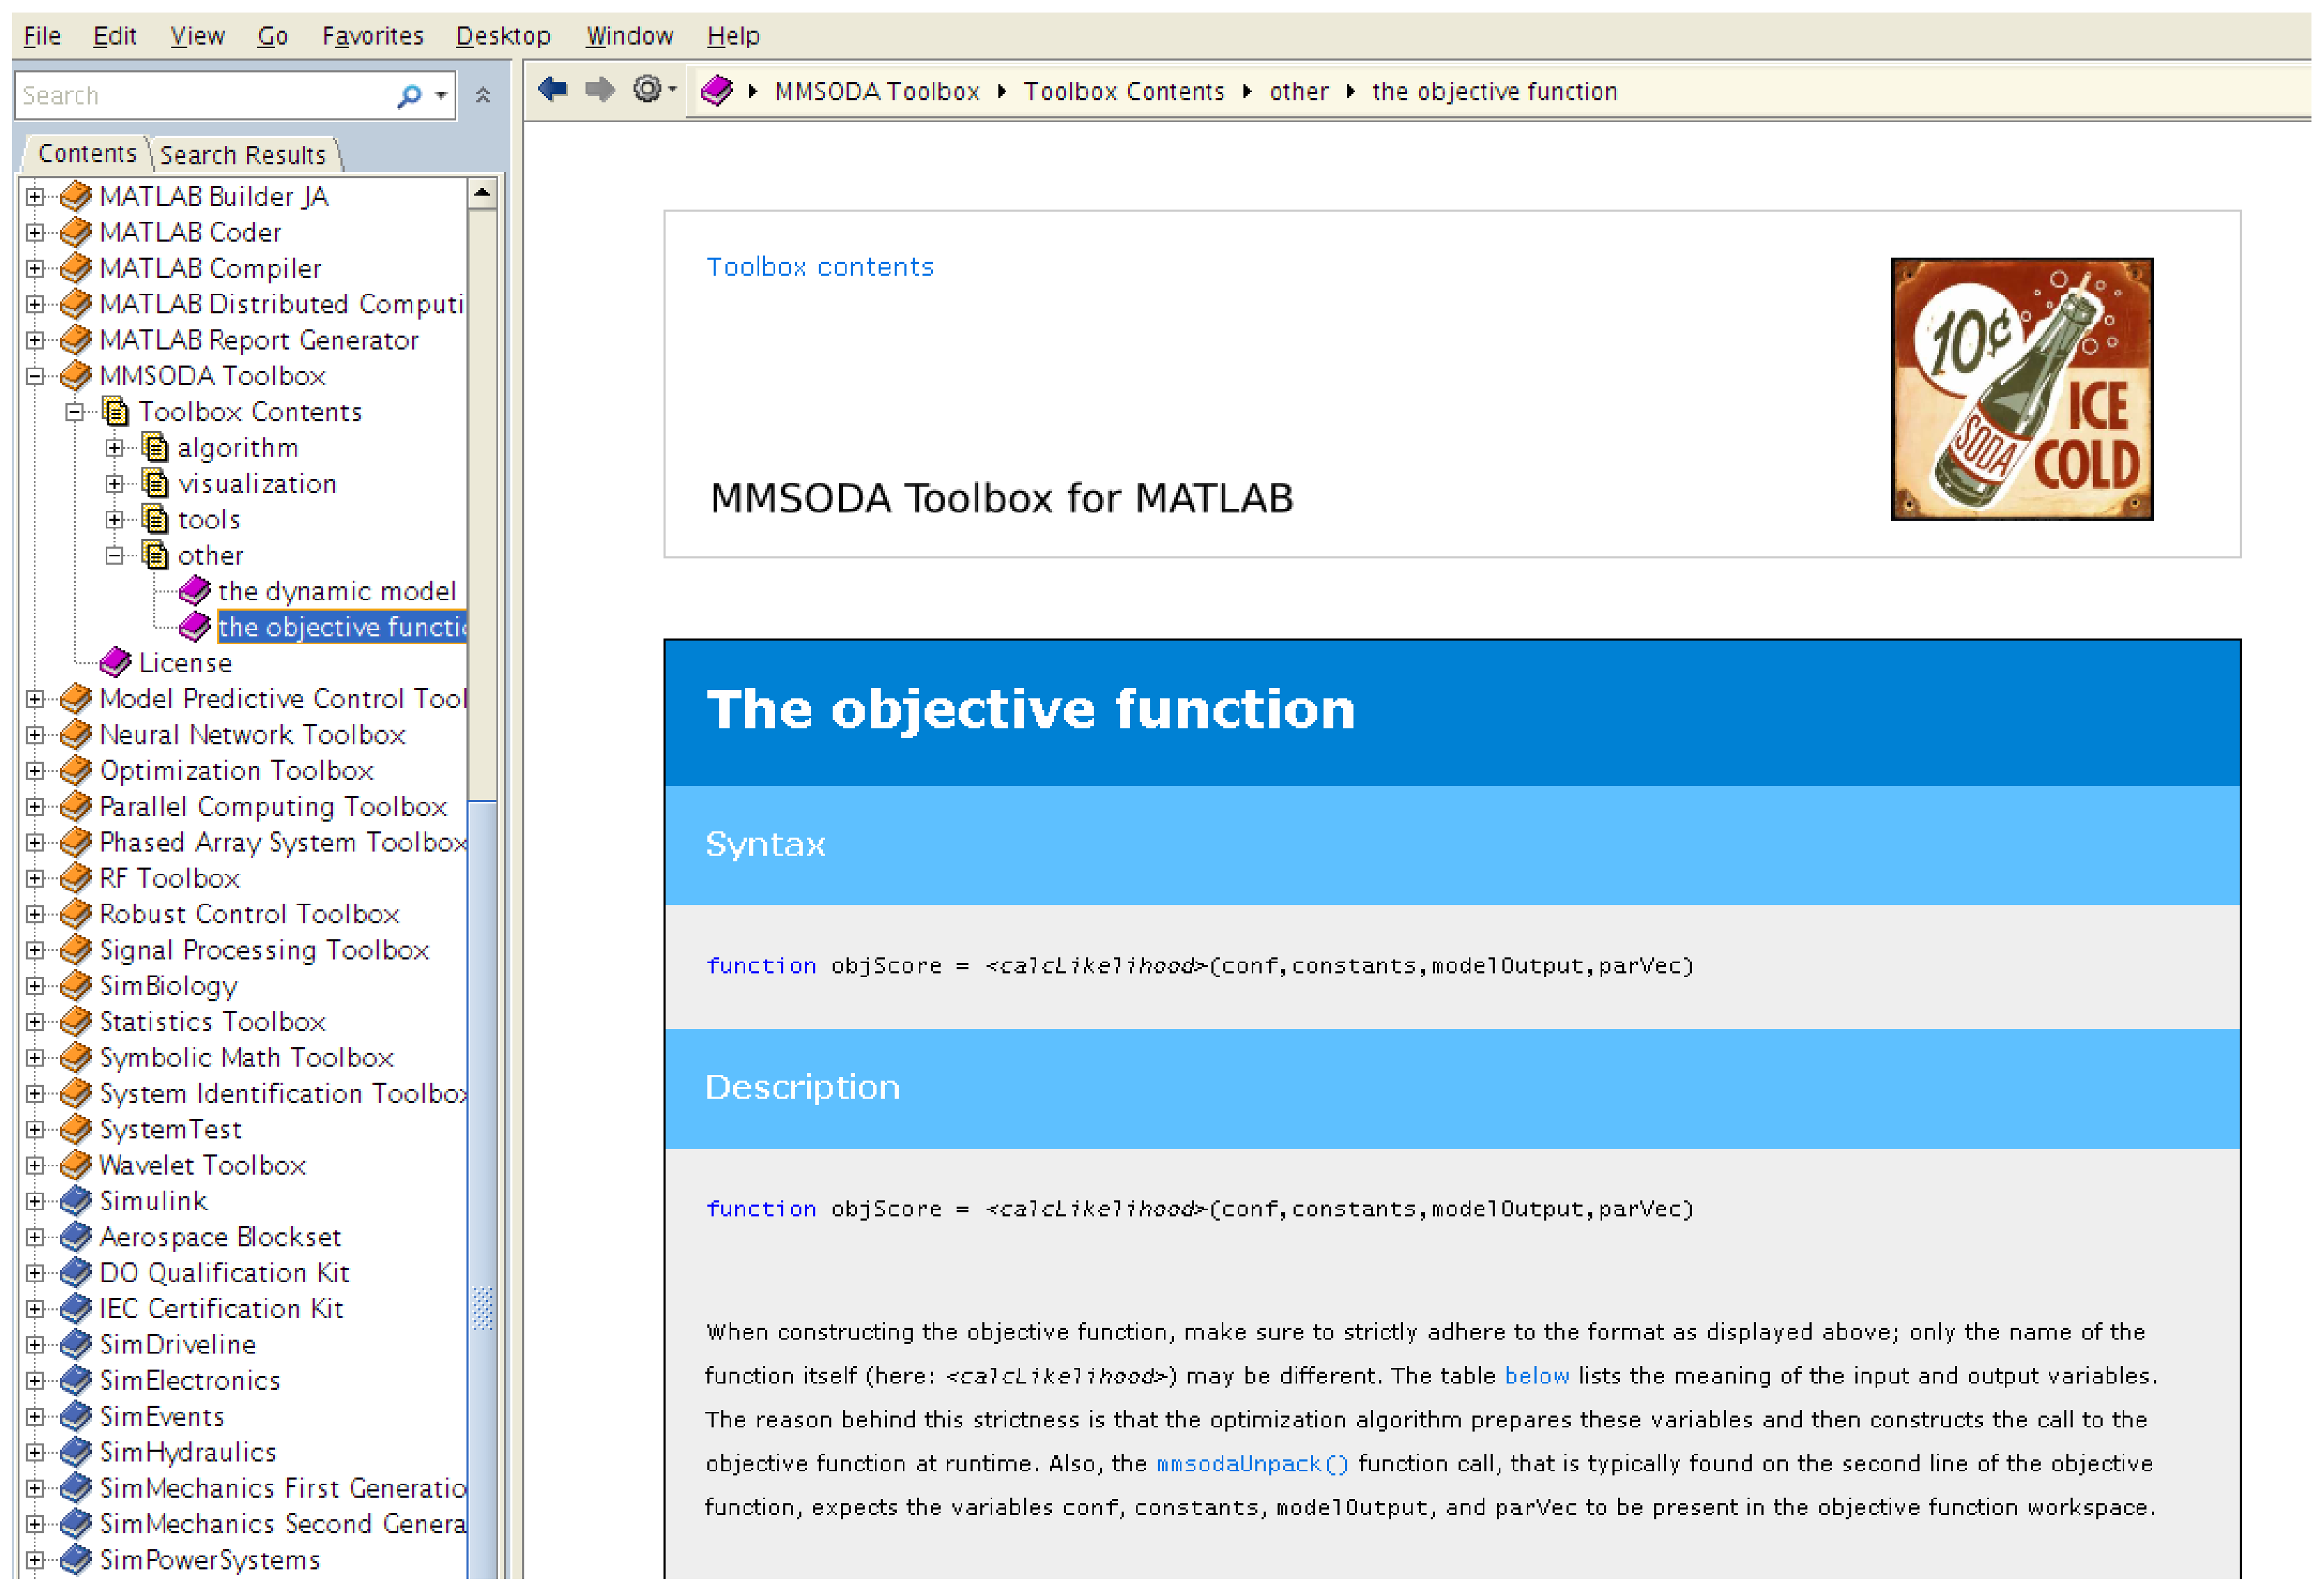
\includegraphics[width=\linewidth,keepaspectratio]{./../eps/doc-the-objective-function.eps}
  \caption{MATLAB documentation on how to set up the objective function.}
  \label{fig:doc-the-objective-function}
\end{figure}

\smallq{Create a new m-file in the `./model' subdirectory, and call this file `calcLikelihoodState.m'. Refer to the documentation and make sure the first line of the objective function is correct.}

The objective function we will use is related to the sum of squared residuals \index{sum of squared residuals} or SSR\index{SSR}:
\begin{equation}\label{eq:SSR}
\mathrm{SSR} = \displaystyle\sum\limits_{t=1}^{n_o}(\hat{x}_{t}-\tilde{x}_{t})^2
\end{equation}
with $\hat{x}_{t}$ the $t^{\mathrm{th}}$ predicted value of $x$, $\tilde{x}_{t}$ the $t^{\mathrm{th}}$ observed value of $x$, and $n_o$ the total number of observations. Note that the number of observations $n_o$ is one less than the number of elements in \texttt{conf.nPrior}, since the first column in \texttt{modelOutput} is not calculated by the model, but instead contains the initial values of the model output variables.

However, we can't use the SSR directly as an objective score, because the SSR is not a log-likelihood (or a probability, for that matter). This problem is easily resolved though, by using the following objective function\footnote{Skip forward to Appendix~\ref{ch:likelihoods-in-optimization} to see how this was derived.}:
\begin{equation}\label{eq:objScore}
\ell = -\frac{1}{2} \cdot{} n_o \cdot{} \mathrm{ln}\left(\mathrm{SSR}\right)
\end{equation}

In order to calculate the SSR, we need some observations. These have been prepared already and are located in the `other' directory.

\smallq{Copy `other/lintank-obs.mat' to your `./data' directory.}

\smallq{In `calcLikelihoodState.m', add \\
\texttt{load({\squote{./data/lintank-obs.mat}},\squote{obs},\squote{obsTimes})}
}% smallq


Now that we have the observations in the workspace, we still need to select the corresponding simulations from the \texttt{modelOutput} variable. Refer to the documentation on the objective function for a description. We want to select all values pertaining to the first state (since this is the state that we have observations for). We can do so by:

\needspace{5\baselineskip}

\begin{lstlisting}[style=basic,style=matlab]
% row of interest in 'modelOutput' is #1
r = 1;
nPriors = size(modelOutput,2);
nObs = nPriors-1;

% extract the relevant row from 'modelOutput'
sim = modelOutput(r,1:nPriors);

% Calculate the SSR, but ignore the first entry in 'obs' and 'sim' because those are always
% exactly the same anyway
ssr = sum((obs(1,2:nPriors)-sim(1,2:nPriors)).^2);

% use the SSR to calculate the likelihood
objScore = -(1/2) * nObs * log(ssr);
\end{lstlisting}

\smallq{Add the command lines above to your \texttt{calcLikelihoodState} in order to let it calculate the SSR and the objective score according to Eq.~\ref{eq:objScore}.}

\smallq{Make sure you are still in the right working directory. At the MATLAB prompt, type:\\
\texttt{>> [evalResults,critGelRub,sequences,metropolisRejects,conf] = mmsoda()}\\
}


Currently, \texttt{calcLikelihoodState} loads the observations from file every time it needs to calculate the \texttt{objScore}. Since file operations are much slower than memory operations, it is more efficient to load the observations just once (during creation of the constants), and then keep them in the computer's memory.

\smallq{Cut the \texttt{load} statement from \texttt{calcLikelihoodState} and paste it into `makeconstants.m'. Make sure to re-run \texttt{makeconstants()}, otherwise `./data/constants.mat' will remain unchanged.}

\smallq{Re-read the documentation on MMSODA's \texttt{mmsodaUnpack()} function. Go back to `calcLikelihoodState.m' and use \texttt{mmsodaUnpack()} to make the observations available in the objective function's workspace. Restart the optimization to check if everything works.}


%\smallq{\textit{some interpretation of results}.\index{todo}}

\section{MMSODA in `scemua' mode; parallel execution}

\smallq{Generate a `Makefile' and a jobscript using \texttt{mmsodaPrepParallelFiles()}. Use the same answers as those given on page~\pageref{li:answers-mmsodaPrepParallelFiles}. }

\smallq{Copy the working directory to LISA using WinSCP or an alternative program. Make sure the directory is at the same level as the `mmsoda-toolbox' directory that should still be present on the remote system.}

\smallq{Use PuTTY to start an SSH connection to the LISA cluster.}

\smallq{Load the necessary software modules and compile your m-files together with the MMSODA m-files.}

\smallq{Add the executable permission to `run-mmsoda.sh'.}

\smallq{Start the optimization on the login node.}

So far, we've run our optimizations on one of the login nodes. These nodes are intended for testing small problems and for development work. However, if you want to do some real calculations, then it becomes necessary to submit your job to the PBS queue (as discussed in Chapter~\ref{ch:getting-started}).

\smallq{Submitting your optimization to the PBS scheduler requires a slightly different jobscript. On your local system, run \texttt{mmsodaPrepParallelFiles}, but this time indicate that you want to run your optimization as a PBS jobscript, without much verbal feedback, and that you want 00:15:00 walltime on 1 node. We are not interested in saving the timings for the moment. When \texttt{mmsodaPrepParallelFiles} finishes, it prints the name of the file it just created (`jobscript-mmsoda.pbs') to the command window. Copy this file to the working directory on the remote system.}


\smallq{Make sure that PuTTY is in the right directory and type:\\
\texttt{qsub jobscript-mmsoda.pbs}\\
to add the optimization to the scheduler's queue. Note that it is not necessary to change the permission bits for `jobscript-mmsoda.pbs' when it is simply an input argument to \texttt{qsub}, rather than a program in its own right. Furthermore, it is also not necessary to re-compile your program, since we did not change anything in the code---we're just submitting to a different queue.}

\smallq{Use the tools discussed in Chapter~\ref{ch:getting-started} (e.g.\,\texttt{qstat}, \texttt{showq}, \texttt{showstart}, \texttt{checkjob}) to check on the status of your job.}

%\smallq{When the job has finished, copy the contents of the `./results' subdirectory to your local system for further analysis.}

\subsection{Standard output and standard error}

This is probably as good a time as any to look in more detail at some of the outputs that MMSODA generates. On the remote machine, there should now be a file `./results/jobscript-mmsoda.pbs.\textbf{o}XXXXXXX' (those X's represent the job id number). This file contains the standard \textbf{o}utput of our parallel optimization program. Whenever any of the parallel processes would normally print some message to the command window, on LISA that text will instead end up in the standard output file\index{standard output file}. The standard output file (and its sister, the standard \textbf{e}rror file\index{standard error file} `./results/jobscript-mmsoda.pbs.\textbf{e}XXXXXXX') is interesting because it is the first place to look if something is not going like it should.

It is not necessary for you to fully understand what all lines in the standard output mean, but having just a general idea can save you a lot of time and frustration when you run into trouble. Most often, tracking an error is just a matter of spotting the difference between the output that you see when everything is working and when it's not. If nothing else, you can send the standard output file to one of the LISA administrators, such that (s)he may assist you better in solving your problem.

The standard output files that are generated during MMSODA optimizations typically consist of three parts: first, there is the output that was written when everything was being set up for the MMSODA run; second, there is a middle part that contains output that would be displayed in MATLAB's command window if you were running MMSODA on your local machine. Finally, the third part contains some text that the LISA system adds to every job's standard output. Listings~\ref{li:standard-out-first-part} and \ref{li:standard-out-last-part} show the most interesting parts of the standard output for a single-objective MMSODA optimization in `scemua' mode. Much of the lines in the first part are generated by bash commands\footnote{See page~\pageref{word:bash} in Chapter~\ref{ch:getting-started}.} from the jobscript. For example, it includes the ID of the job (lines 3--4), an \texttt{ls -l} overview of the files in the current directory (lines 12--22), an overview of the type of CPU in each node (lines 29--45), an overview of the nodes which have been assigned to this job by the scheduler (lines 47--63; the name of each node occurs as many times as there are CPUs in it, so in this case there are 16 `r41n3' entries). Then the necessary modules are loaded and an overview is printed of the available modules (lines 65--77). Next, lines 79--81 add the current directory to the environment variable LD\_LIBRARY\_PATH to make sure that `libmmpi.so' can be located by the compiled MATLAB program. The next few lines (83--85) prepare a temporary directory that is needed by the compiled MATLAB program. Lines 87--117 print results of the Linux \texttt{ldd}\index{Linux commands!ldd@\texttt{ldd}} command. \texttt{ldd} prints the location of the libraries that are needed by our compiled MATLAB program (`matlabprog') and by the library that we made (`libmmpi.so'). After every \texttt{=>} sign in the \texttt{ldd} result, there should be an entry; if it says `not found', something is wrong. For example, if we would not have added the current directory to the LD\_LIBRARY\_PATH, line 91 would say `\texttt{libmmpi.so => not found}'. Next, lines 119--176 constitute a list of so-called `symbols' that are present inside the `mmsoda-toolbox/comms/helper.o' file. This file is a C-language object file needed for MPI communication between nodes in the cluster. The next few lines (178--195) show that the MATLAB engine was indeed started 16 times (once for every CPU in the node), and each of those 16 instances of MATLAB recognized immediately that there was no display (since the nodes inside a cluster are primarily set up for calculation, and are therefore not connected to a screen).


The middle part of the standard output is what you normally see in the command window; it starts with a disclaimer message that is generated by the MMSODA code (lines 197--198). Most of the remainder of the middle part consists of `Evaluating parameter sets X-Y' messages (lines 203--902), indicating the progress of the MMSODA algorithm.

The last part of the standard output file (lines 906--920) is always added by the LISA system. It provides an overview of the resources that were used in executing the job.

\Needspace{15\baselineskip}

\lstinputlisting[style=basic,style=bash,style=numbered,style=spacious,breaklines=true,breakindent=0,breakautoindent=false,prebreak=\mbox{{\color{blue}\hspace*{1em}$\swarrow$}},postbreak=\mbox{{\color{blue}$\rightarrow$\hspace*{1em}}},caption={First part of the standard output file. Lines that were too long to fit on the page were wrapped; this is indicated with the line break \mbox{{\color{blue}$\swarrow$}} and line continuation \mbox{{\color{blue}$\rightarrow$}} symbols.},label=li:standard-out-first-part,firstline=1,lastline=207]{./../res/jobscript-mmsoda.pbs.o6734963}

\Needspace{15\baselineskip}

\lstinputlisting[style=basic,style=bash,style=numbered,style=spacious,breaklines=true,breakindent=0,breakautoindent=false,prebreak=\mbox{{\color{blue}\hspace*{1em}$\swarrow$}},postbreak=\mbox{{\color{blue}$\rightarrow$\hspace*{1em}}},caption={Last part of the standard output file. Lines that were too long to fit on the page were wrapped; this is indicated with the line break \mbox{{\color{blue}$\swarrow$}} and line continuation \mbox{{\color{blue}$\rightarrow$}} symbols.},label=li:standard-out-last-part,firstline=898,lastline=920,firstnumber=898]{./../res/jobscript-mmsoda.pbs.o6734963}



\subsection{Analyzing the parallelization overhead}

When dealing with parallel programs, it is often useful to monitor how much time is lost in parallelization overhead in relation to the CPU time (recall Fig.~\ref{fig:walltime-comparison}). The MMSODA Toolbox for MATLAB enables you to record and visualize the timings of all relevant events (sending and receiving data, serializing\index{serializing}\footnote{Serialization is the process of collecting all the arrays that need to be sent over to a different machine, such that the arrays occupy a consecutive part of the computer's memory. This part of the memory can then be sent to another machine.} and deserializing\index{deserializing}, waiting for input, etc.) on all nodes that have been assigned to the job. Recording the timings does slow the optimization down slightly, so the default behavior is not to record any events. However, enabling the time-keeping functionality is simply a matter of re-running the \texttt{mmsodaPrepParallelFiles()} function, and answering `a : yes' to the last question `Would you like to save the timings?'.

\smallq{Re-run \texttt{mmsodaPrepParallelFiles()} and enable time-keeping. Copy the newly created jobscript to the cluster. Submit the new jobscript using \texttt{qsub}.}

\smallq{After the job finishes, copy the contents of the `./results' directory from the remote system to your local system.}


\smallq{Read the documentation on \texttt{mmsodaAnalyzeTimings}\index{MMSODA functions!mmsodaAnalyzeTimings@\texttt{mmsodaAnalyzeTimings}} and visualize the timings for the linear tank example. Would you say that parallel optimization of the linear tank model is a coarse-grained or a fine-grained problem?}

At this point, you are familiar with MMSODA in `bypass' mode and in `scemua' mode, and you know how to run MMSODA optimizations locally as well as on the LISA cluster. In the next few sections, we will cover the `reset' mode and `soda' modes, but the important point is that the workflow as you know it from the previous projects (as summarized in Fig.~\ref{fig:mmsoda-workflow}) is the same for all MMSODA projects.

\begin{figure}[htbp]
  \centering
    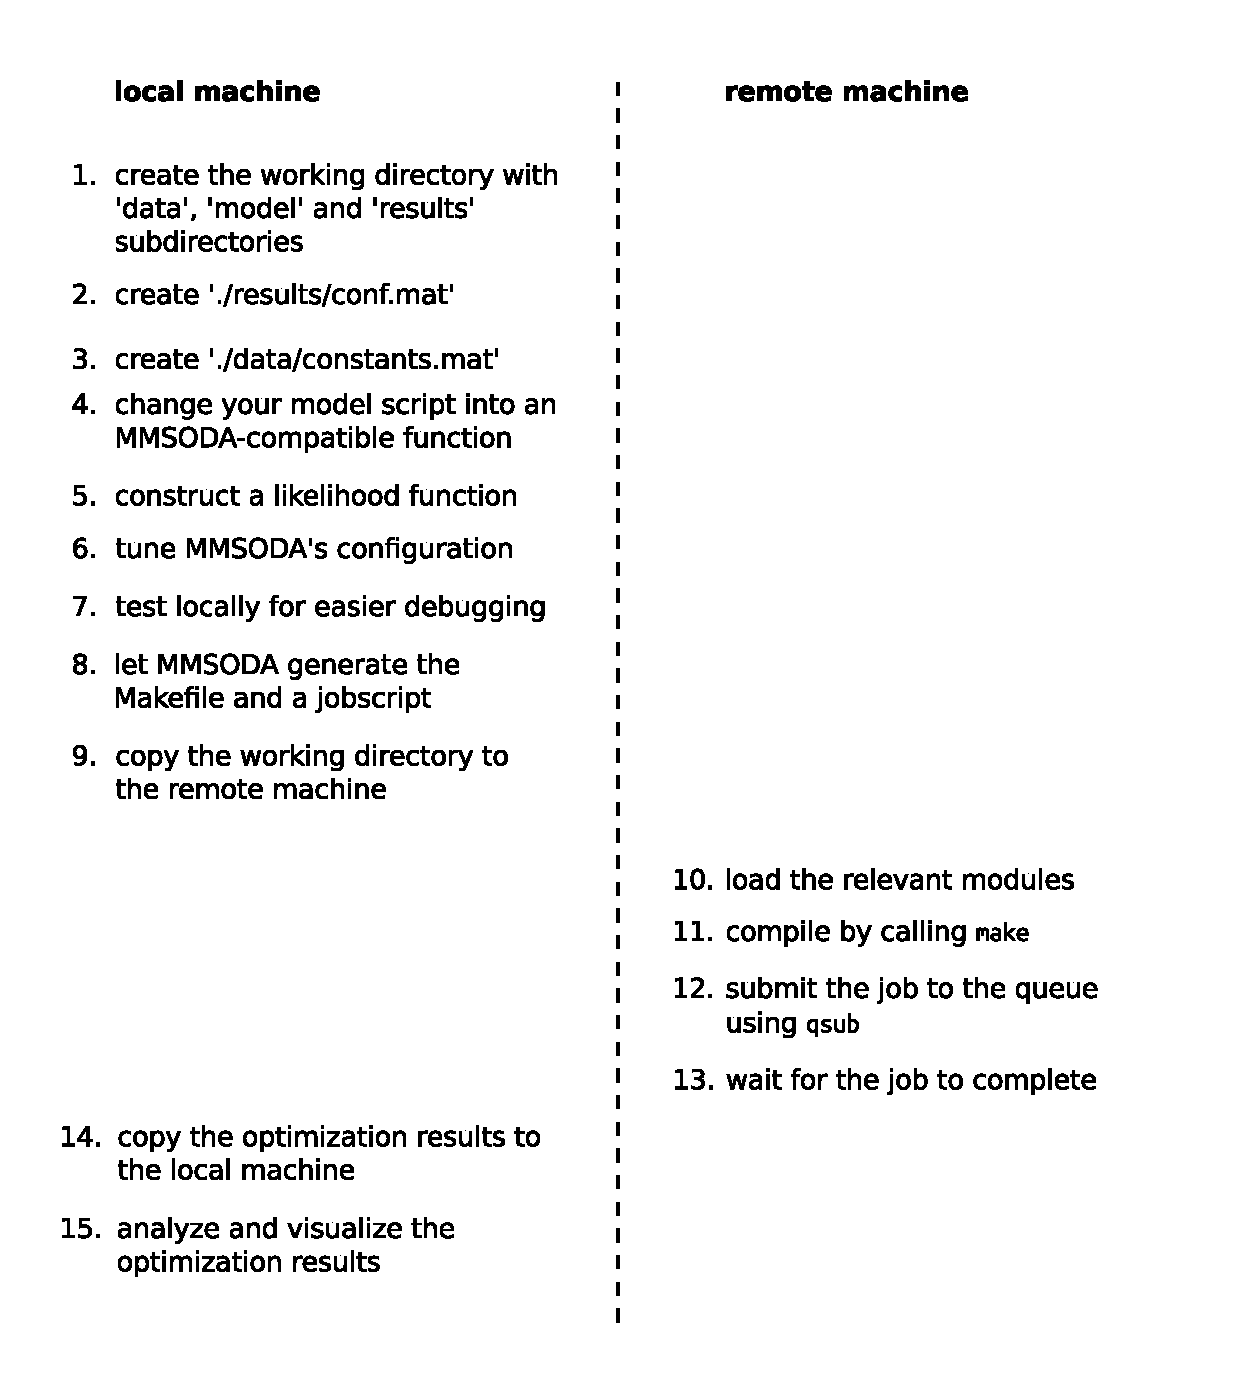
\includegraphics[width=0.85\linewidth,keepaspectratio]{./../eps/mmsoda-workflow.eps}
  \caption{Typical workflow for setting up MMSODA optimizations. Note that the items under `remote machine' are executed in a terminal program such as PuTTY.}
  \label{fig:mmsoda-workflow}
\end{figure}


\smallq{Now that you know what information goes where for MMSODA in `scemua' mode, it may be useful to review some of the other examples in the `esibayes-master' directory. On your local machine, explore the configurations for a few of the other `scemua' mode directories. Run MMSODA for those configurations, but make sure MATLAB is set to the correct working directory when \texttt{mmsoda} is started.}


\section{MMSODA in `reset' mode; sequential execution}

\smallq{On your local system, make a copy of the `example2' directory, and rename the copy to `example3'. Clean up the `example3' directory by removing `matlabprog', `libmmpi.so', `Makefile', `jobscript-mmsoda.pbs' as well as any results pertaining to the `example2' case. Set your MATLAB working directory to the newly created `example3' directory.}

\smallq{Remove the `constants.mat' and `lintank-obs.mat' files from the `example3/data' directory. Copy `lintank-obs-unobserved-input.mat' from the `other' directory to `example3/data'.}

\smallq{On the MATLAB command line, load the \texttt{obsTimes} and \texttt{obs} variables from the `./data/lintank-obs-unobserved-input.mat' file by typing:\\
\texttt{ >> load(\squote{./data/lintank-obs-unobserved-input.mat},\squote{obsTimes},\squote{obs})}}

\smallq{Visualize the data that were just loaded by:\\
\texttt{ >> plot(obsTimes,obs(1,:),\squote{-b.})}\\
Your figure should be similar to Fig.~\ref{fig:lintank-obs-unobserved-input}.}

\begin{figure}[htb]
  \centering
    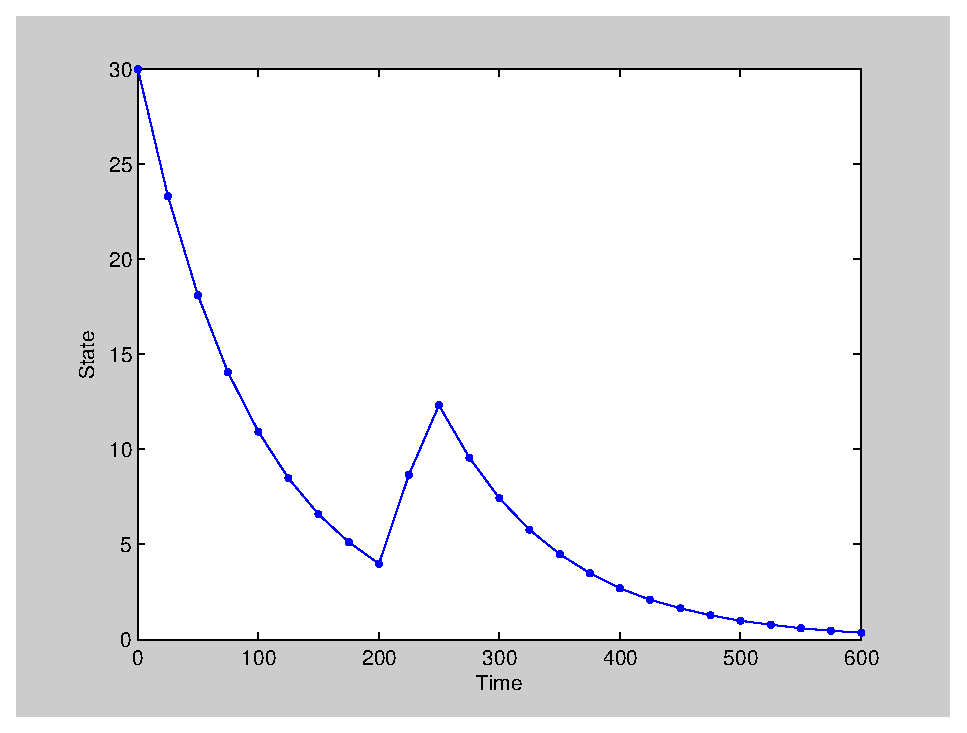
\includegraphics[width=\linewidth,keepaspectratio]{./../eps/lintank-obs-unobserved-input.eps}
  \caption{Simple \texttt{plot} of the data in `./data/lintank-obs-unobserved-input.mat'. The true value of the resistance parameter in this figure is 100.}
  \label{fig:lintank-obs-unobserved-input}
\end{figure}

From Fig.~\ref{fig:lintank-obs-unobserved-input}, it is clear that something happened around Time=200--250. It seems that water was added to the upper tank---that is to say, the upper tank has been subjected to an unobserved input. This kind of error is very common in hydrology; for example if the linear tank simulates the streamflow from a particular catchment, it can sometimes happen that streamflow in the river increases (as in Fig.~\ref{fig:lintank-obs-unobserved-input}), without any rain being recorded during the preceding days. Most often, these kinds of apparent impossibilities are explained by a rainstorm which did indeed pass over (some of) the catchment, but which missed the location of the rain gauge. Observational error like that can play havoc with the effectiveness of the calibration, as we shall see shortly.

In this section, we will look at what happens if we take a naive approach to calibrating the lintank model to the data of Fig.~\ref{fig:lintank-obs-unobserved-input}. For this, we need to make a few changes in the MMSODA configuration. For example, we need the model to generate predictions at \texttt{priorTimes = [0:25:600]}, and we want to use the data from `./data/lintank-obs-unobserved-input.mat' in the objective function.

\smallq{Make the necessary changes to `makeconf.m' and `makeconstants.m' to implement these changes. Also change the value of the \texttt{dtSimDefault} model constant to 2.0 and set the lower and upper boundaries of the parameter space to 10 and 500, respectively. Furthermore, set the \texttt{doPlot} configuration variable to \texttt{true}, such that MMSODA will produce some standardized visualizations as the optimization progresses. Finally, set \texttt{nModelEvalsMax} to \texttt{7000}.}

\smallq{Run the updated versions of `makeconf.m' and `makeconstants.m' and verify that the necessary files are created. Then, start the \mbox{SCEM-UA} optimization in the regular way from the MATLAB command window.}

Listing~\ref{list:calcUncertaintyIntervals} on page~\pageref{list:calcUncertaintyIntervals} demonstrates how parameter uncertainty intervals can be constructed using the information in \texttt{evalResults}. A copy of the listing has been included as `calcUncertaintyIntervals.m' in the `./other' directory.

\Needspace{5\baselineskip}

\smallq{Study the script and use it to visualize the model prediction for the best parameter set, along with the parameter uncertainty intervals for the case of Fig.~\ref{fig:lintank-obs-unobserved-input}.}

\Needspace{45\baselineskip}

\lstinputlisting[style=basic,style=matlab,style=numbered,style=spacious,caption={Simple MATLAB script that demonstrates how parameter uncertainty intervals can be constructed from the information in \texttt{evalResults}. A copy of this script has been included as `other/calcUncertaintyIntervals.m'.},label=list:calcUncertaintyIntervals]{./../m/calcUncertaintyIntervals.m}

As you can see from the resulting figure, optimizing the model without allowing for the unobserved input to the upper tank can lead to biased parameter estimates---even though the best parameter set minimizes the residuals, the corresponding model output is plainly wrong. In the rest of this section, we will look at data assimilation. Data assimilation provides a way of dealing with uncertain model states (for example as a result of uncertain model forcings, initial state or model structure error). MMSODA supports two types of data assimilation: in the first, full confidence is placed on the observation, i.e.\,whenever the simulated time reaches a time at which an observation is available, the model state pertaining to that time (known as \textit{prior}\index{prior state}\index{state!prior} state or \textit{forecast} state\index{forecast state}\index{state!forecast}) is abandoned, and the value of the model state is reset to the value of the observation. In MMSODA parlance, this mode is known as the `reset' mode\index{MMSODA!reset mode}. The second type of data assimilation that MMSODA supports is the `soda' mode, which we will study in greater detail in section~\ref{sec:soda-mode}.


According to \texttt{mmsoda}'s documentation, the following configuration variables are required for running MMSODA in `reset' mode when using one objective (we do not use \texttt{initMethodNOKF}, \texttt{initValuesNOKF} and \texttt{namesNOKF} since we are only interested in the model state for the moment and do not bother with any additional variables):

\begin{multicols}{2}
\begin{enumerate}
\item{\texttt{initMethodKF}}
\item{\texttt{initValuesKF}}
%\item{\texttt{initMethodNOKF*}}
%\item{\texttt{initValuesNOKF*}}
\item{\texttt{modeStr}}
\item{\texttt{modelName}}
%\item{\texttt{namesNOKF*}}
\item{\texttt{objCallStr}}
\item{\texttt{obsState}}
\item{\texttt{parNames}}
\item{\texttt{parSpaceHiBound}}
\item{\texttt{parSpaceLoBound}}
\item{\texttt{priorTimes}}
\item{\texttt{stateNamesKF}}
\item{\texttt{stateSpaceHiBound}}
\item{\texttt{stateSpaceLoBound}}
\item[]{}
\end{enumerate}
\end{multicols}

As you can see, you are already familiar with most of these, but there are a few new ones as well. \texttt{initMethodKF} and \texttt{initValuesKF} always go together. Their purpose is to initialize the correct initial values to those state variables which are subject to state updating. For our case, that means that \texttt{initMethodKF} must be set to \texttt{\squote{reference}} (this is currently the only supported method), and that \texttt{initValuesKF} must be set to \texttt{30.0} (the initial value of the \texttt{state1} variable). This implies that \texttt{state1Init} no longer needs to be part of the model constants, and that \texttt{state1} no longer needs to be initialized by assigning \texttt{state1Init}  to \texttt{state1} in `lintank.m'.

Configuration variable \texttt{obsState} is used to tell MMSODA what the observed values of the state are for every time in \texttt{priorTimes}. For our case, that means that \texttt{obsState} must be assigned the values from variable \texttt{obs} from `./data/lintank-unobserved-input.mat'.

You also have to indicate which model variables you want to be part of the Ensemble Kalman Filter scheme (Note that we are using the simplest scheme here, i.e.\,the `reset' scheme). This is done through the \texttt{stateNamesKF} variable, which is simply a list of variable names as they are used in the model. We only have one variable, so you need to set \texttt{stateNamesKF} to \texttt{\{\squote{state1}\}}.

Finally, you need to specify the limits on the state space, i.e.\,for each state, you define what the maximum and minimum values are, using \texttt{stateSpaceHiBound} and \texttt{stateSpaceLoBound}, respectively. For this data set, reasonable values are 40.0 and 0.0, respectively.

\smallq{Make the necessary changes to `makeconf.m', `makeconstants.m', and `lintank.m'. Start the `reset' mode optimization from the command line like you did before. MMSODA will most likely not run just yet; a couple of things need to be resolved first. Interpret the error messages and make the required changes until MMSODA will start without any errors.}

\smallq{Once the optimization completes after 7000 model evaluations, use `calcUncertaintyIntervals.m' to visualize the parameter uncertainty (but change the name of the *.mat file from `scemua-so-results.mat' to `reset-so-results.mat'). If the result is not quite what you hoped it would be; don't worry, this is just because `calcUncertaintyIntervals.m' does not reset the values of the prior states when constructing the uncertainty intervals. Luckily, there is an easy way around this problem.}

\smallq{Read the description of the \texttt{saveEnKFResults} and \texttt{startFromUniform} configuration variables in \texttt{mmsoda}'s documentation.}

\smallq{Change `makeconf.m' such that it will evaluate an additional 500 parameter combinations. Make sure to set \texttt{startFromUniform} to \texttt{false} (we want to resume the previous run) and set \texttt{saveEnKFResults} to \texttt{true}, to be able to plot uncertainty intervals for the prior state values later on. Re-run `makeconf.m' and start the optimization as usual.}


\smallq{When the additional 500 parameter sets have been evaluated, verify that you have a bunch of new files in the `./results' directory, whose names are formatted like `reset-so-results-enkf-evals-Z-Z.mat', with Z representing an integer number.}

\smallq{Read the documentation on \texttt{mmsodaPlotEnsemble}\index{MMSODA functions!mmsodaPlotEnsemble@\texttt{mmsodaPlotEnsemble}}. Make a new figure using \texttt{mmsodaSubplotScreen(2,2,1)} and visualize the prior state values associated with the last parameter combination.}

\smallq{Once that works, try to visualize the last 20 parameter sets using \texttt{mmsodaPlotEnsemble}'s optional parameters.}

As you can see, there are quite a few parameter combinations that do not result in a very good fit. It would seem then that the uncertainty intervals associated with these model outputs are quite large. This is not the case, though; it is simply because the default behavior for \texttt{mmsodaPlotEnsemble} is to include all model outputs in the figure, regardless of whether they were accepted or rejected by the Metropolis part of MMSODA. If you want to view only the model outputs that were accepted by the Metropolis part of MMSODA, you should use \texttt{mmsodaPlotEnsemble}'s \texttt{\squote{replaceRejected}} optional parameter.

\smallq{Make a new figure using \texttt{mmsodaSubplotScreen(2,2,2)}. Visualize the same selection of parameter combinations as you did previously, but this time, let \texttt{mmsodaPlotEnsemble} replace the rejected outputs with model outputs that were accepted. Note that the model evaluation number in the figure's title is no longer simply \texttt{[7481:7500]} but instead shows the model evaluation numbers that replaced the Metropolis-rejected ones.}

\smallq{Make a new figure using \texttt{mmsodaSubplotScreen(2,1,2)}. Use \texttt{mmsodaMatrixOfScatter} to plot the evaluation number on the x-axis against the parameter value on the y-axis for the last part of the record (see optional parameter \texttt{\squote{nHistory}}). Use the resulting figure to verify that \texttt{mmsodaPlotEnsemble} replaced the correct model outputs.}

Now that we have some idea about what sort of model outputs are probable, let's calculate the 95\% parameter uncertainty intervals. MMSODA comes prepackaged with a function that retrieves the correct model outputs from the relevant files in `./results' and that calculates time series of arbitrary percentiles, while taking into account the intermediate state updating that has been performed by MMSODA.

\smallq{Read the MMSODA documentation on \texttt{mmsodaCalcUncertInts}\index{MMSODA functions!mmsodaCalcUncertInts@\texttt{mmsodaCalcUncertInts}} and use it to calculate the 2.5\%, 50\% and 97.5\% percentiles. The code snippet in Listing~\ref{list:patch-uncertainty-snippet-reset} may serve as an example of how \texttt{mmsodaCalcUncertInts}'s result may be used, while Fig.~\ref{fig:result-of-patch-uncertainty-snippet-reset} shows what the result looks like.}


\Needspace{30\baselineskip}

\lstinputlisting[style=basic,style=matlab,style=numbered,style=spacious,caption={MATLAB code snippet for visualizing parameter uncertainty intervals for the lintank model. A copy of this script has been included as `other/patch\_uncertainty\_snippet.m'.},label=list:patch-uncertainty-snippet-reset]{./../m/patch_uncertainty_snippet.m}

\begin{figure}[htb]
  \centering
    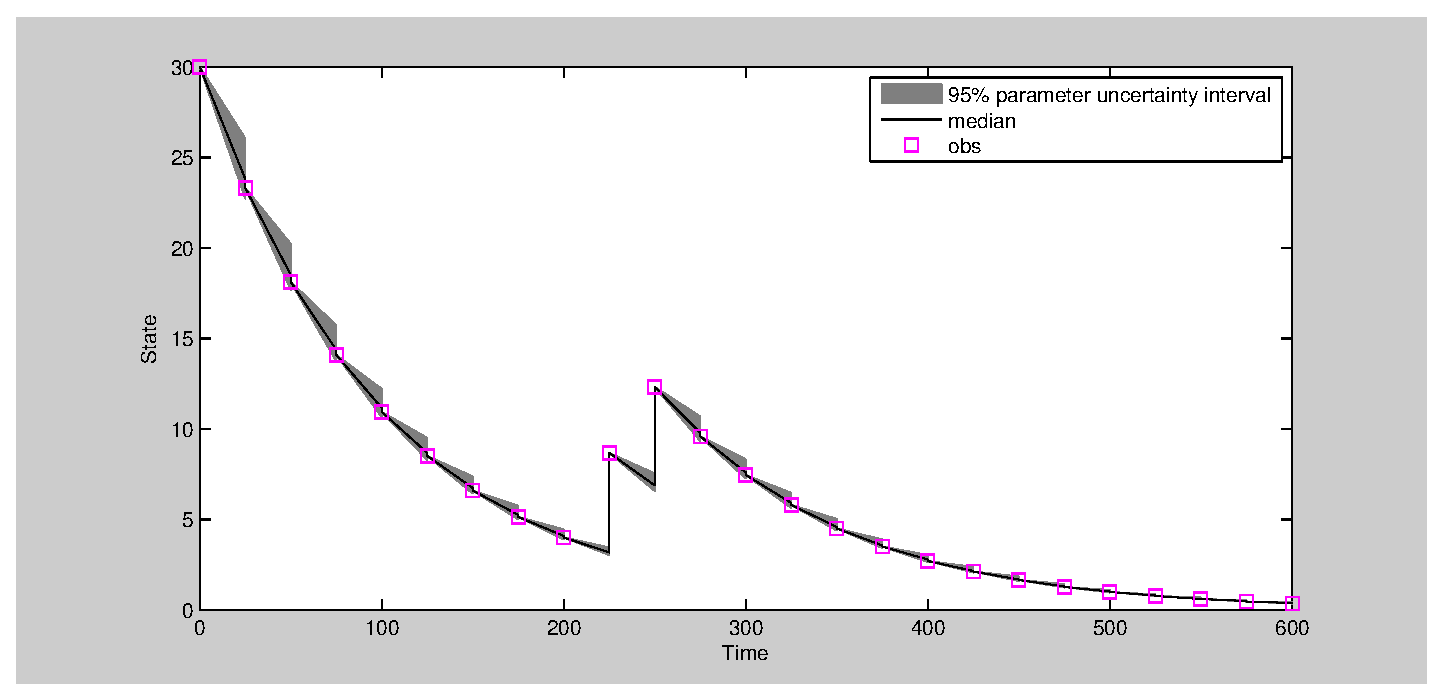
\includegraphics[width=\linewidth,keepaspectratio]{./../eps/result-of-patch-uncertainty-snippet-reset.eps}
  \caption{Result of running the code from Listing~\ref{list:patch-uncertainty-snippet-reset}.}
  \label{fig:result-of-patch-uncertainty-snippet-reset}
\end{figure}


%\section{MMSODA in reset mode; parallel execution}

%\smallq{Refer to Fig.~\ref{fig:mmsoda-workflow} in order to run the `example3' case on the LISA cluster.}

\section{MMSODA in `soda' mode; sequential execution}
\label{sec:soda-mode}
\index{MMSODA!soda mode}


\smallq{On your local machine, copy the `example3' directory to a new directory, `example4'. Clean up the `./results' subdirectory, and remove `matlabprog', `libmmpi.so', and `Makefile', as well as any jobscripts pertaining to `example3'.}

The `soda' mode is the most complex and most compute-intensive mode. It is similar to the `reset' mode in that it updates the model states during the simulation. The way the updating is performed, however, is different. The difference between `scemua', `reset', and `soda' modes essentially comes down to how much confidence is placed on the observed values of the state in comparison to how much confidence is placed on the simulated values of the state. For example, in `scemua' mode, all of the confidence is placed on the simulated values---the model can be run from the time of the initial state (\texttt{conf.priorTimes(1)}) to the time at which the last prediction is required (\texttt{conf.priorTimes(end)}), without the need for temporarily halting the model at \texttt{conf.priorTimes(2:end-1)} to do any state updating. In contrast to this, the `reset' mode places full condidence on the observations: at the times when an observation is available, the model is temporarily halted, and its states are reset to the value of the observed state. The `soda' mode then, provides sort of a middle ground between MMSODA's `scemua' and `reset' modes: instead of placing all of the confidence on one or the other, a little confidence is placed on both the simulated and the observed value of the states. A weighted average of the two is then calculated, and the simulated state (i.e.\,the prior state\index{prior state}\index{state!prior}) is adjusted in the direction of the observed state. The magnitude of the adjustment is sometimes referred to as the `state \textit{innovation}'\index{state!innovation} or simply `state \textit{update}'\index{state!update}. Adding the state update to the prior state results in a new state value, which is known as the `\textit{posterior} state'\index{posterior state}\index{state!posterior} or the `\textit{analysis} state'\index{analysis state}\index{state!analysis}.

%\textit{explanation of weighting prior state and obs if std or var are known. (i.e. normal Kalman Filter)\index{todo}}

%\textit{extend explanantion of weighting if the equations are not linear. the information is then stored by perturbing the prior and pertubing the obs, and then weighting them together.\index{todo}}

In terms of setup, the `soda' mode is not so different from the `reset' mode that you are familiar with. In fact, a quick look at the table of configuration variables in \texttt{mmsoda}'s documentation reveals that only 3 additional configuration variables are needed: \texttt{covObsPert}, \texttt{covModelPert}, and \texttt{nMembers}.

\smallq{Read the description in \texttt{mmsoda}'s documentation for these three options.}

\smallq{Include \texttt{covObsPert}, \texttt{covModelPert}, and \texttt{nMembers} in your `makeconf.m', and assign them values of \texttt{0.02}, \texttt{0.10} and \texttt{10}, respectively. Don't forget to change \texttt{modeStr} to \texttt{\squote{soda}}, otherwise MMSODA will overwrite the values of \texttt{covObsPert} and \texttt{covModelPert} with \texttt{0}. Set \texttt{nModelEvalsMax} to \texttt{150} for now, re-run `makeconf.m', and verify that `./results/conf.mat' was indeed written.}


\smallq{Re-read the documentation on the objective function (see Figure~\ref{fig:doc-the-objective-function}), in particular the description of the input argument \texttt{modelOutput}, which is 3-D if \texttt{modeStr} is \texttt{\squote{soda}}.}

\smallq{Adapt the objective function such that the SSR is calculated based on the ensemble-member mean of the prior state. Note: calculating the mean over the 3$\mathrm{^{rd}}$ dimension of an N-dimensional array \texttt{X} in MATLAB is easily achieved by \texttt{mu = mean(X,3)}.}

\smallq{Test your configuration locally until it works. Then set \texttt{nModelEvals} to \texttt{7000} and re-run `makeconf.m'.}

\smallq{Call \texttt{mmsodaPrepParallelFiles} to write the jobscript and the Makefile.}

\smallq{Copy your `example4' working directory to the cluster.}

%how does one determine the values of covobspert and covmodelpert?

\section{MMSODA in `soda' mode; parallel execution}

\smallq{Use PuTTY to set up an SSH connection to the LISA cluster. Make sure the necessary modules are loaded before compiling the binary. Submit your jobscript to the queue and wait for the optimization to finish.}

\smallq{Once the job finishes, edit `makeconf.m' on your local machine by setting \texttt{saveEnKFResults} to \texttt{true} and \texttt{startFromUniform} to \texttt{false}. Increase the maximum number of model evaluations by \texttt{500}. Run \texttt{makeconf} and copy the new MMSODA configuration to the remote system. Submit the jobscript to the queue once more, and wait for the results.}

\smallq{Copy the optimization results back to your local machine.}

\smallq{Copy the code snippet from Listing~\ref{list:patch-uncertainty-snippet-reset} to your working directory. Adapt the filename from which the optimization results are read, and run the snippet on the results of the `soda' mode optimization. The result should look like Fig.~\ref{fig:result-of-patch-uncertainty-snippet-soda}.}


\begin{figure}[htb]
  \centering
    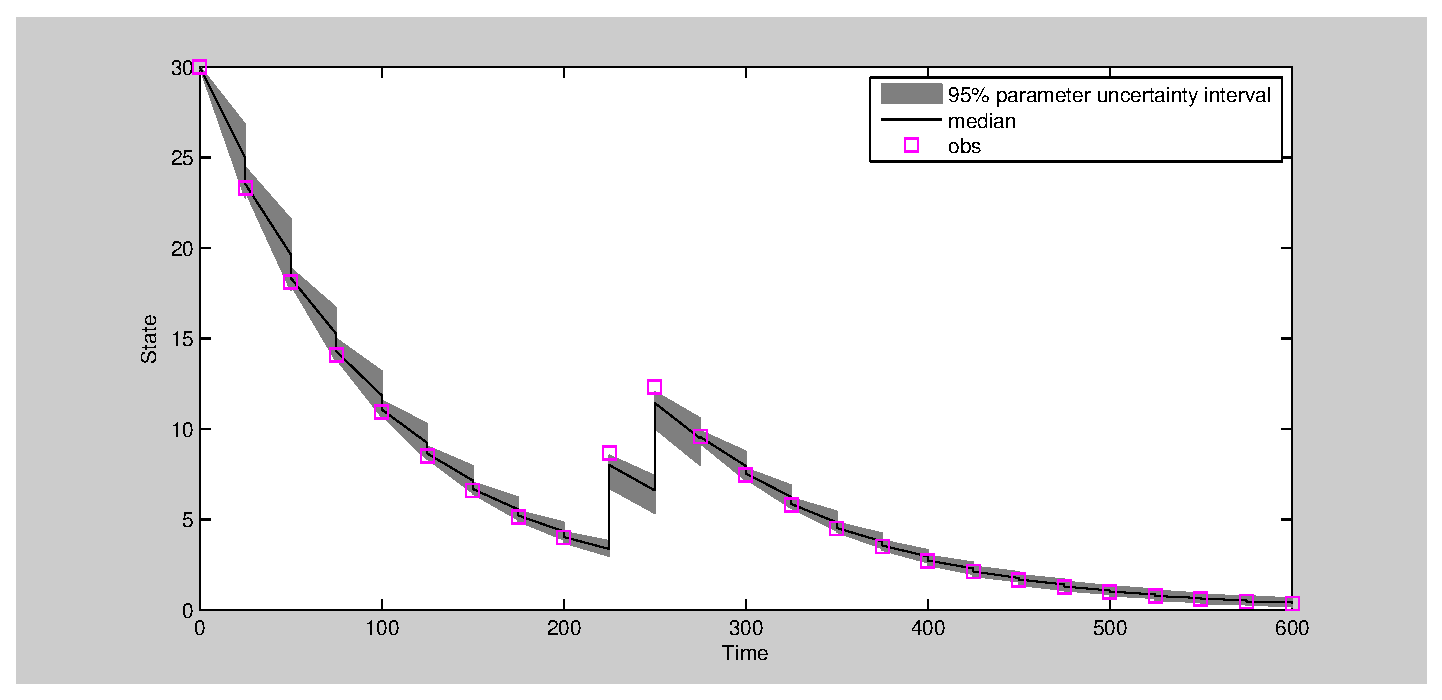
\includegraphics[width=\linewidth,keepaspectratio]{./../eps/result-of-patch-uncertainty-snippet-soda.eps}
  \caption{Parameter uncertainty intervals for the `soda' mode optimization of the lintank model.}
  \label{fig:result-of-patch-uncertainty-snippet-soda}
\end{figure}




\chapter{Remote graphical applications}

% This chapter explains how to start graphical applications on a remote computer, such that you can interact with its graphical interface locally.


Up to this point, we've issued commands through the terminal.  The terminal is a powerful tool, but sometimes it's also useful to run graphical programs\index{graphical programs} (as opposed to text-based terminal programs) remotely, for example when you want to use the graphical debugging capabilities that the MATLAB GUI offers to debug some of your code on LISA, or if you want to view remotely generated MATLAB figures.
%Within the context of optimization, another typical application of running graphical applications remotely is that you can have the LISA system generate figures, for instance showing the progress of the optimization using visualization routines such as \texttt{mmsodaMatrixOfScatter()}. These figures can then be viewed and manipulated (e.g.~zooming, panning) from your local machine.
Amazingly, this is possible through a process called \textit{X forwarding over SSH}\index{X!forwarding over SSH}. Here, `X'\index{X} refers to the program that takes care of visualization on Linux. The Linux operating system is telling X what to visualize, and then X figures out which pixels on what screen should be what color, and whether a particular pixel is part of, say, a button, drop-down list, or some other user interface element. It is possible to re-route messages to the X system through your SSH connection, such that they end up on your local machine. If your local system is Linux, the X messages that your system receives can be interpreted by your local copy of the X program, and the user interface of graphical application that is running on the remote machine will be displayed locally. However, you are probably running Windows, so you need to install a Windows version of X first.

Download Xming\index{Xming} from \burl{http://sourceforge.net/projects/xming/files/Xming/6.9.0.31/Xming-6-9-0-31-setup.exe/download} and install it. Now go to the Windows start menu and click XLaunch (Fig.~\ref{fig:xlaunch-0}). This will bring up a wizard (Fig.~\ref{fig:xlaunch-1}). Follow the steps outlined in Figs.~\ref{fig:xlaunch-2}--\ref{fig:xlaunch-4}.

\begin{figure}[H]
  \centering
    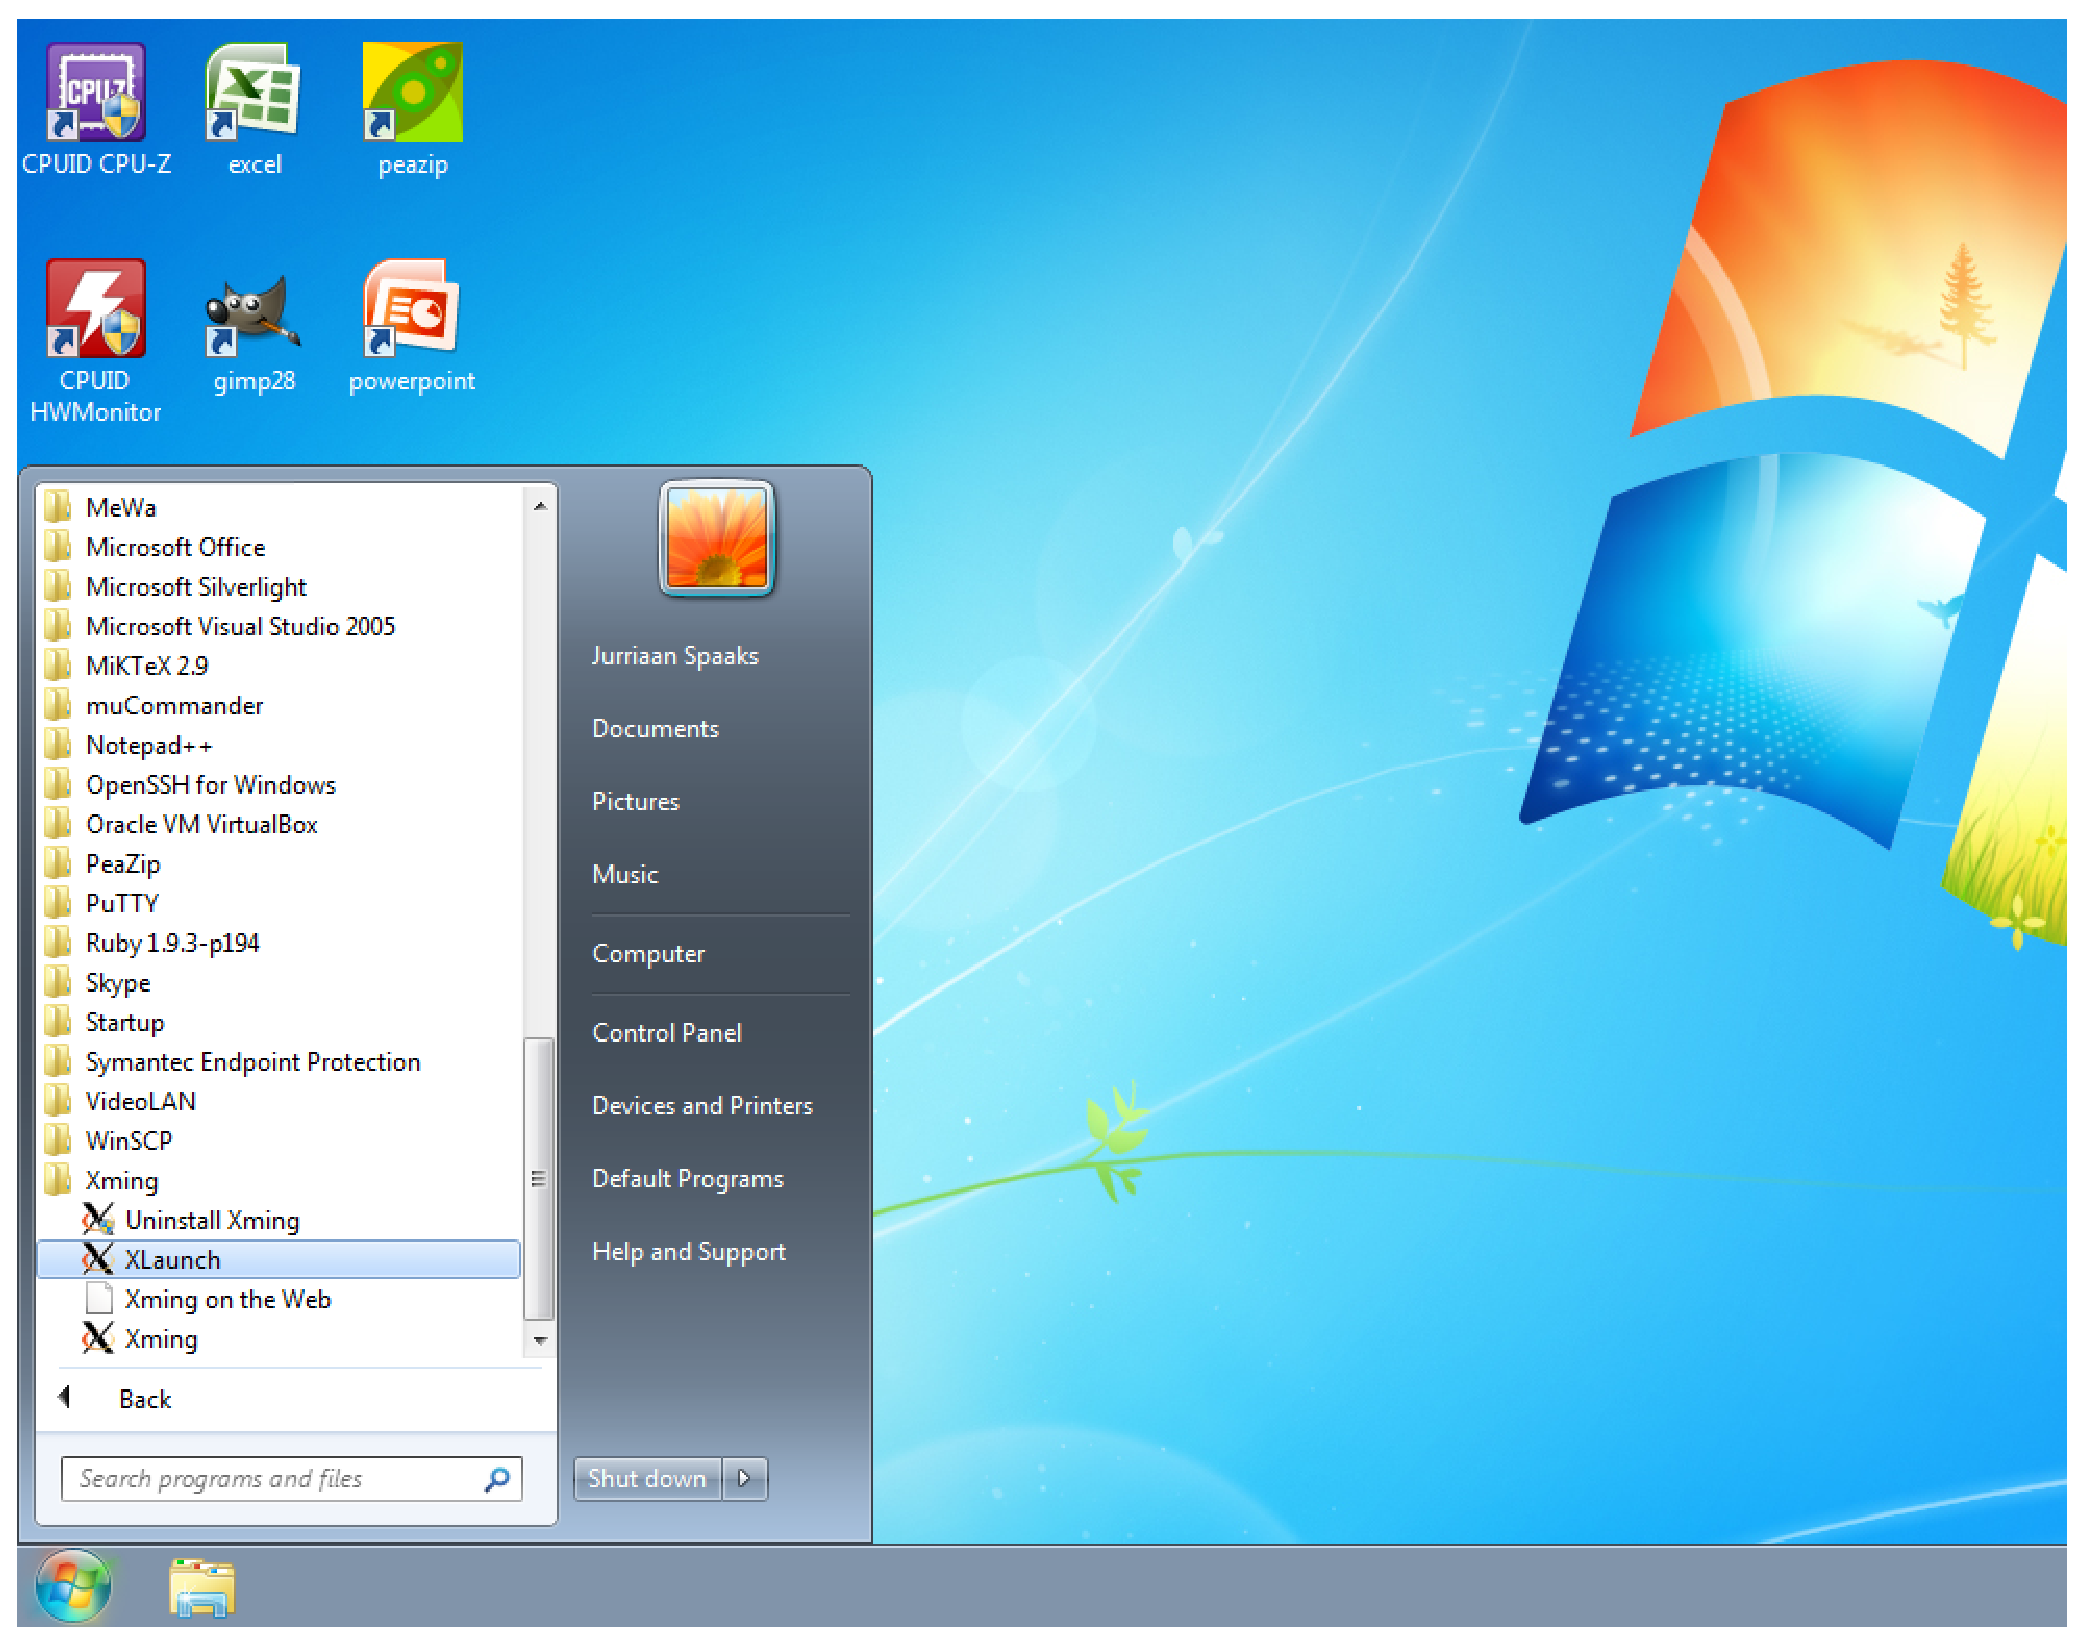
\includegraphics[width=0.8\textwidth]{./../eps/xlaunch-1.eps}
  \caption{Starting XLaunch from the Windows 7 start menu.}
  \label{fig:xlaunch-0}
\end{figure}


\begin{figure}[H]
  \centering
    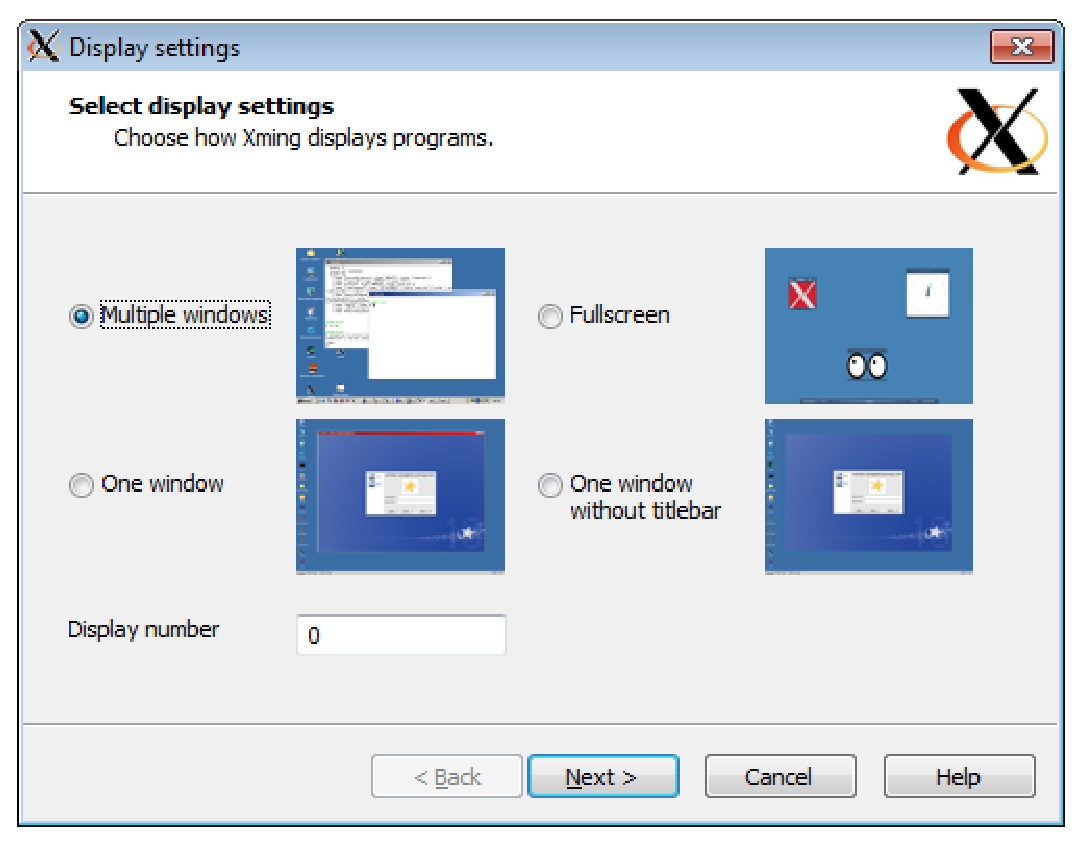
\includegraphics[width=0.7\textwidth]{./../eps/xlaunch-2.eps}
  \caption{The XLaunch configuration wizard page 1.}
  \label{fig:xlaunch-1}
\end{figure}

\begin{figure}[H]
  \centering
    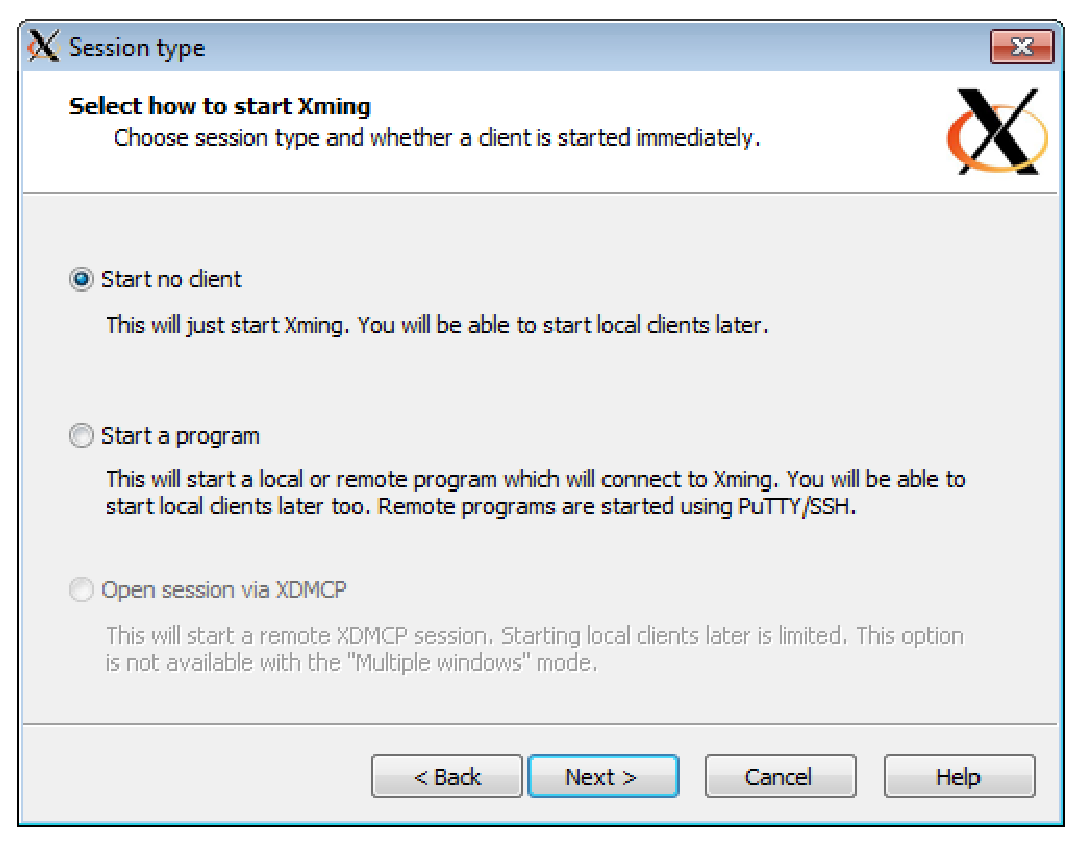
\includegraphics[width=0.7\textwidth]{./../eps/xlaunch-3.eps}
  \caption{The XLaunch configuration wizard page 2.}
  \label{fig:xlaunch-2}
\end{figure}

\begin{figure}[H]
  \centering
    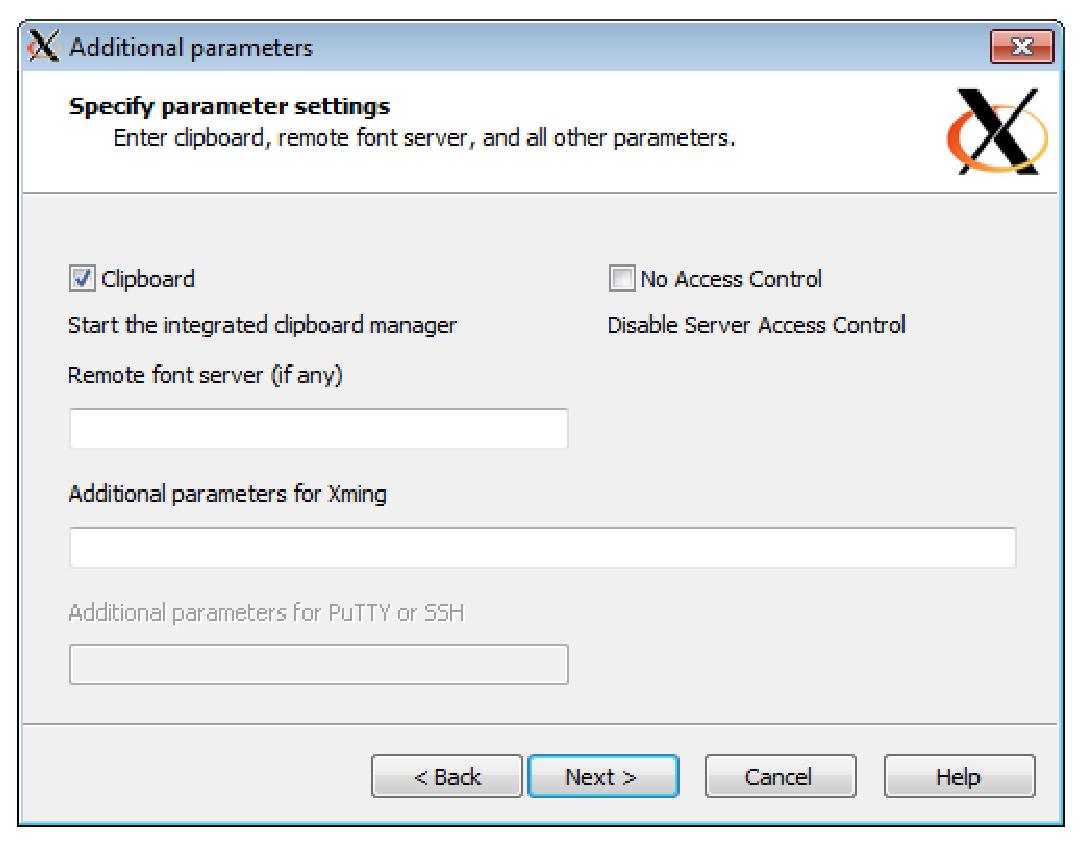
\includegraphics[width=0.7\textwidth]{./../eps/xlaunch-4.eps}
  \caption{The XLaunch configuration wizard page 3.}
  \label{fig:xlaunch-3}
\end{figure}

\begin{figure}[H]
  \centering
    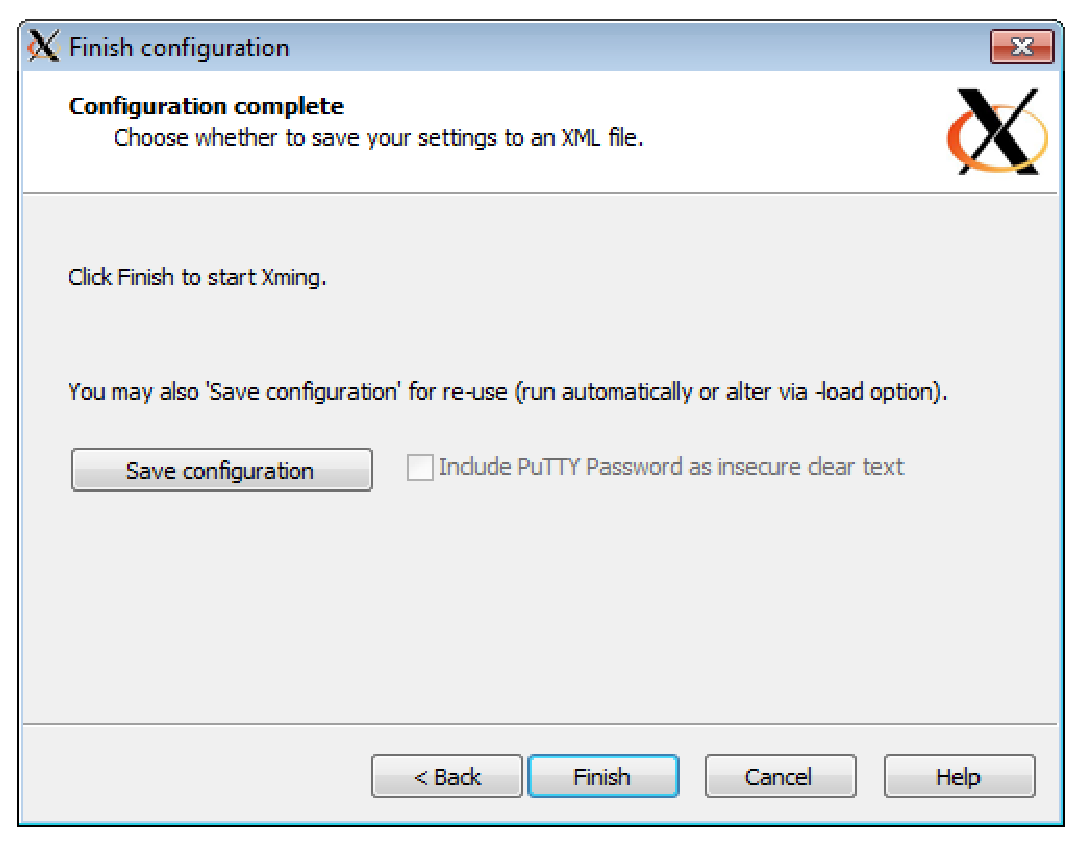
\includegraphics[width=0.7\textwidth]{./../eps/xlaunch-5.eps}
  \caption{The XLaunch configuration wizard page 4.}
  \label{fig:xlaunch-4}
\end{figure}



After you go through the XLaunch wizard, there should be an X icon in your icon tray.

Now that we have an X server for Windows running locally, we still need to tell the remote system that we want it to route its X messages through the SSH connection to our local system. For this, you need to start a new SSH connection. Start PuTTY, and type in the `lisa.sara.nl' host name, exactly as before (recall Fig.~\ref{fig:putty-session-dialog}). However, before clicking the `Open' button, expand the plus sign symbol for `SSH' in the bottom part of the left pane (see Fig.~\ref{fig:putty-x-forwarding}). Find the item labeled `X11' (X is sometimes referred to as `X11'\index{X11}), and in the right pane, enable the checkbox that says `Enable X11 forwarding' before clicking the `Open' button.

\begin{figure}[htb]
  \centering
    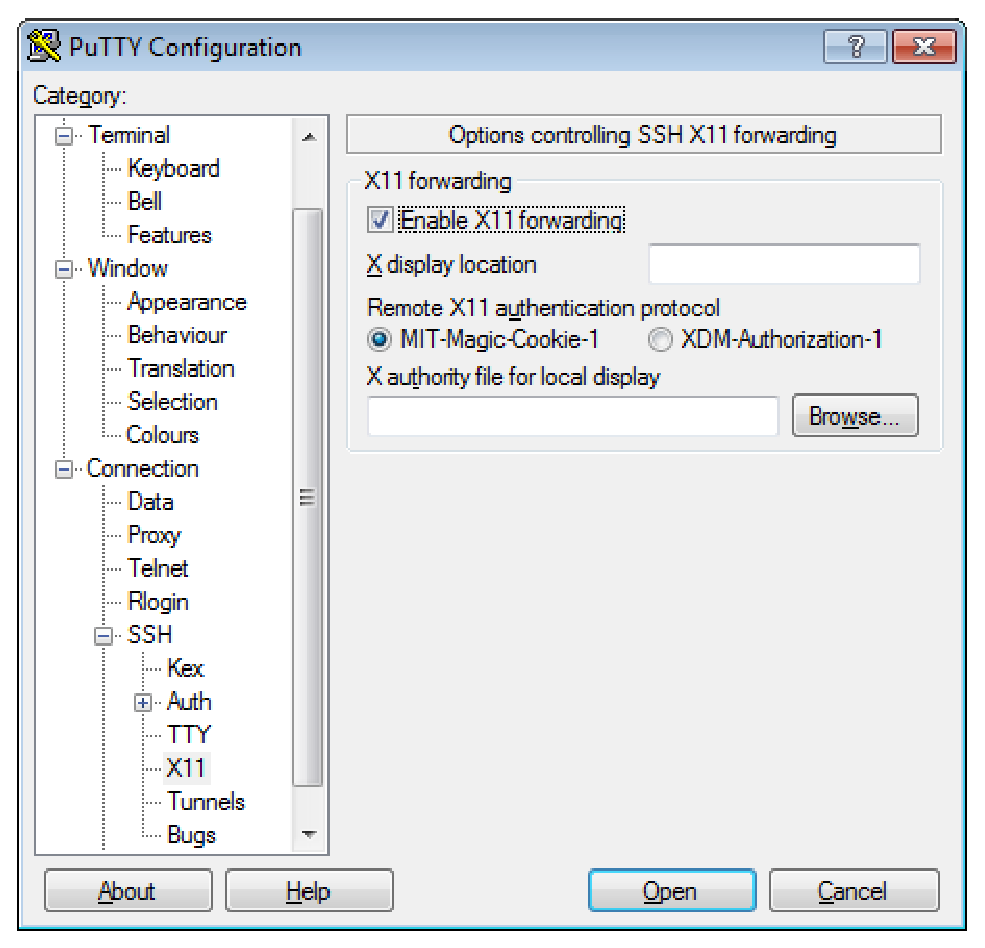
\includegraphics[width=0.6\textwidth]{./../eps/putty-x-forwarding.eps}
  \caption{Configure PuTTY for X forwarding over SSH.}
  \label{fig:putty-x-forwarding}
\end{figure}

At the prompt, you can quickly test whether the remote system is connected to your local X server by typing:
\begin{lstlisting}[style=basic,style=bash]
jspaaks@login4:~$ echo $DISPLAY
\end{lstlisting}\index{Linux commands!echo \char`\$
DISPLAY@\texttt{echo \$DISPLAY}}%Linux commands!echo DISPLAY@\texttt{echo DISPLAY}
which should result in a message like this (the numbers could be different):
\begin{lstlisting}[style=basic,style=bash]
localhost:10.0
\end{lstlisting}
If the connection was unsuccessful, the shell returns an empty message.

Start Octave in silent mode by:
\begin{lstlisting}[style=basic,style=bash]
jspaaks@login4:~$ octave --silent
octave:1>
\end{lstlisting}
and then run the \lstinline[style=bashinline]{peaks(30)} function.
\begin{lstlisting}[style=basic,style=bash]
octave:1> peaks(30)
octave:2>
\end{lstlisting}
After a few moments (depending on the bandwidth of your connection to LISA), it will show you Fig.~\ref{fig:octave-peaks-x-forwarding}.
\begin{figure}[!htb]
  \centering
    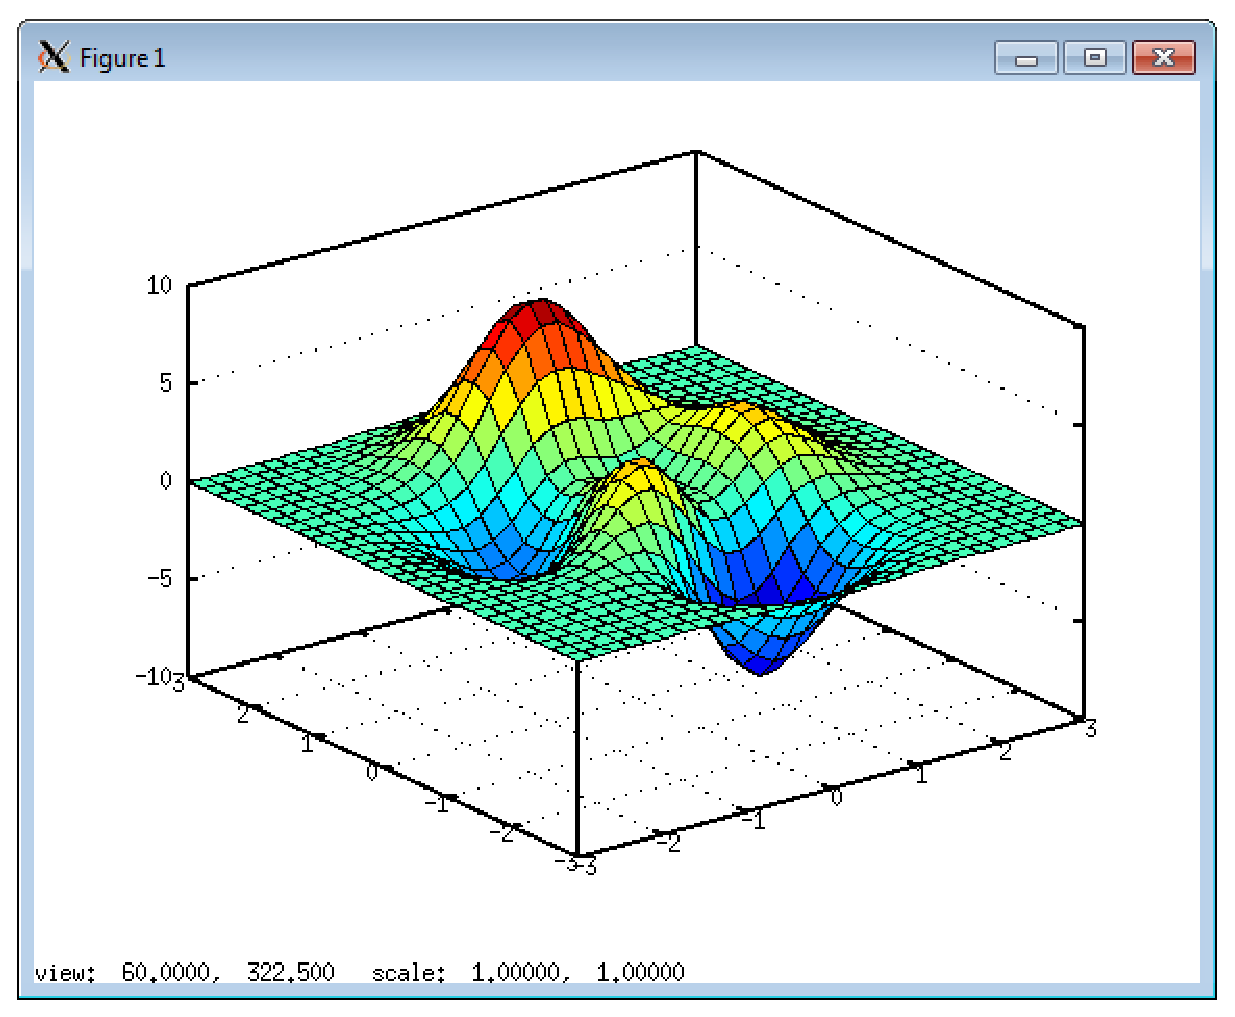
\includegraphics[width=0.6\textwidth]{./../eps/octave-peaks-x-forwarding.eps}
  \caption{After Octave generated this \lstinline[style=bashinline]{peaks(30)} figure remotely, the remote system sent it to the local machine over SSH where it was displayed with Xming.}
  \label{fig:octave-peaks-x-forwarding}
\end{figure}


\needspace{4em}
Let's see if we can do the same thing in MATLAB:
\begin{lstlisting}[style=basic,style=bash]
octave:2> exit

jspaaks@login4:~$ matlab
-bash: matlab: command not found
\end{lstlisting}
The reason this does not work is that MATLAB is only used by some users, therefore it is not available by default\footnote{In fact, you must be a member of the `MATLAB users group' that exist on LISA. Any of LISA's administrators can add you to this group, but it usually involves some administration.}. However, it's easy enough to make MATLAB available, like so:
\begin{lstlisting}[style=basic,style=bash]
jspaaks@login4:~$ module load matlab
jspaaks@login4:~$ matlab
\end{lstlisting}
It is considered good practice to \lstinline[style=bashinline]{unload} MATLAB once you are done with it:
\begin{lstlisting}[style=basic,style=bash]
jspaaks@login4:~$ module unload matlab
\end{lstlisting}
This frees up one of the MATLAB licenses, such that other users may use it. There are currently enough MATLAB licenses to run 32 instances of MATLAB simultaneously; however, some of the toolboxes require a separate license. For some toolboxes there are only 3 licenses available, so if your program happens to use one of those, you can only use 3 MATLAB instances simultaneously.

If you are just using the MATLAB licenses to run your programs on LISA, as opposed to doing development work, you can (legally) circumvent licensing problems by compiling your m-code, and running the compiled code with the \textit{MATLAB Compiler Runtime}\index{MATLAB Compiler Runtime} or \textit{MCR}\index{MCR}. The MCR can be loaded in a similar fashion as the full MATLAB suite:
\begin{lstlisting}[style=basic,style=bash]
jspaaks@login4:~$ module load mcr
\end{lstlisting}
%For more information on compiling code, this is a good starting point: \burl{https://grid.sara.nl/wiki/index.php/Using_the_Grid/Lsg-matlab}

\begin{figure}[!htb]
  \centering
    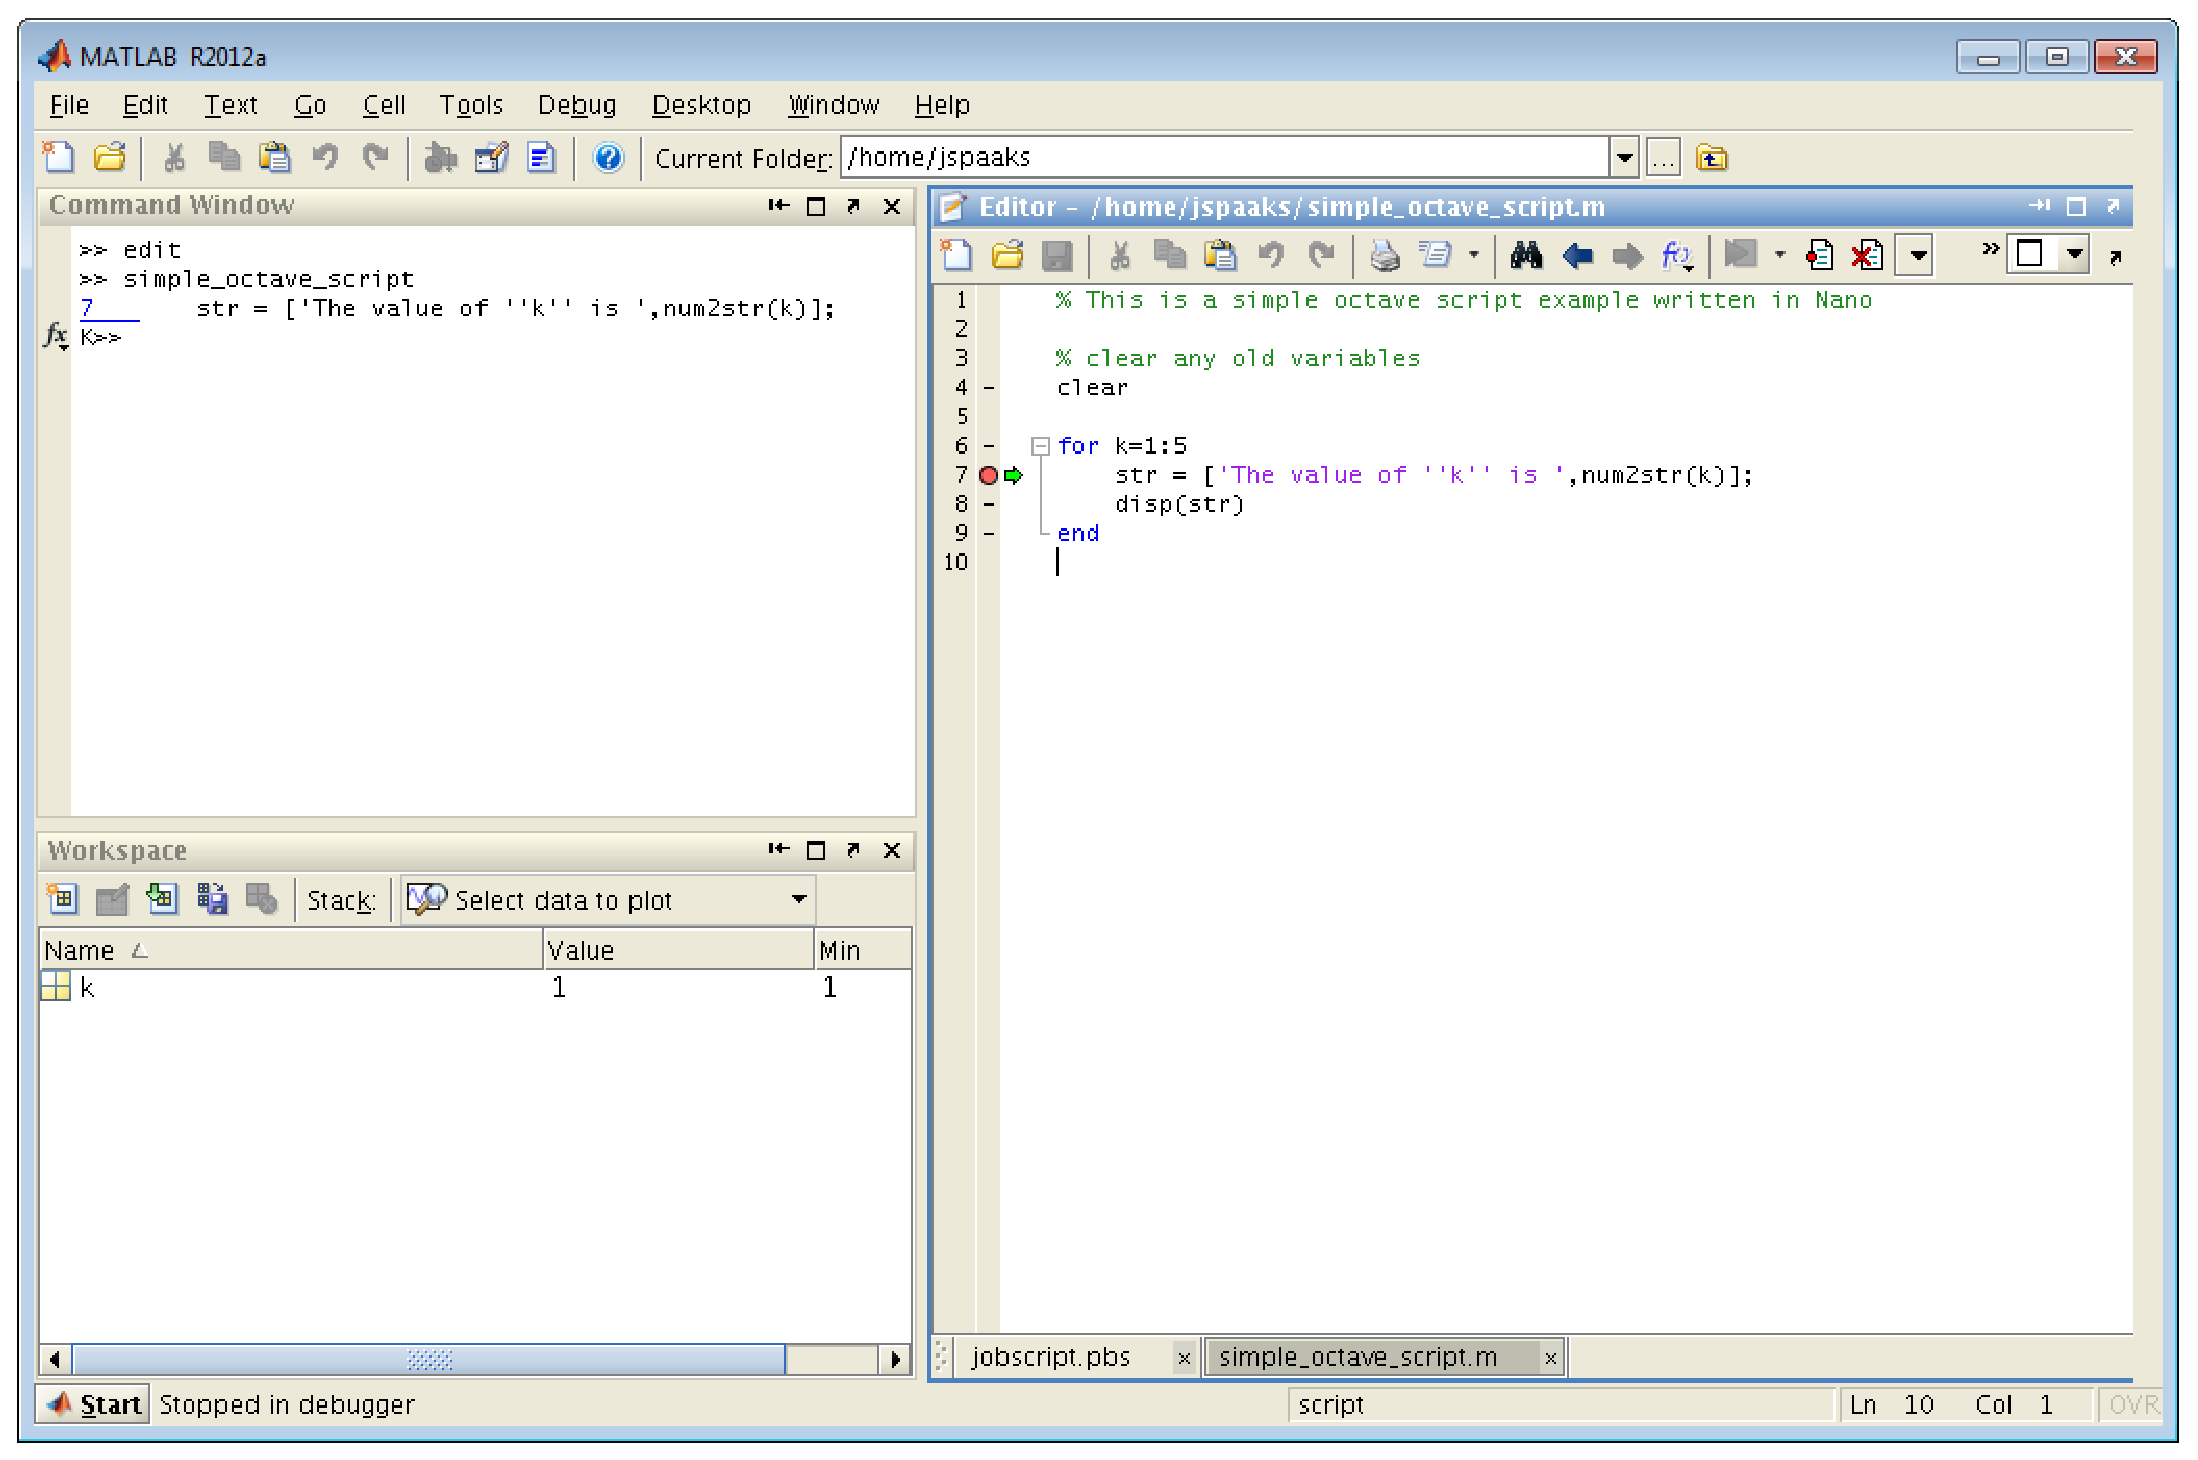
\includegraphics[width=0.9\textwidth]{./../eps/matlab-remote-debugging.eps}
  \caption{Even MATLAB's debugging capabilities can be used remotely!}
  \label{fig:matlab-remote-debugging}
\end{figure}





\chapter{Likelihoods in optimization}
\label{ch:likelihoods-in-optimization}


\section{Definition of the system}


The discrete-time state-space formulation of a nonlinear dynamic system is\footnote{Refer to Appendix~\ref{ch:definition-of-terms} for the meaning of the symbols used in this Chapter.}:

\begin{equation}\label{eq:true-state}
x_{t+1}=f(x_t,u_t,\boldsymbol\theta)
\end{equation}
\begin{equation}\label{eq:true-output}
y_{t+1}=h(x_{t+1},\boldsymbol\phi)
\end{equation}
To keep notation as simple as possible, we consider a system in which the state, the forcing and the output at any given time can be represented as scalars. Further note that the `state' of the system at a given time can include history.
Since it is generally impossible to observe the true state, the true forcing, and the true output of a system, we have to make do with the observed state, observed forcing, and the observed output instead:

\begin{equation}\label{eq:observed-state}
\tilde{x}_{t+1}=x_{t+1} + \omega_{t+1}
\end{equation}
\begin{equation}\label{eq:observed-forcing}
\tilde{u}_{t+1}=u_{t+1} + \psi_{t+1}
\end{equation}
\begin{equation}\label{eq:observed-output}
\tilde{y}_{t+1}=y_{t+1} + \nu_{t+1}
\end{equation}
Note that Eqs.~\ref{eq:observed-state}--\ref{eq:observed-output} assume that the dimensionality of $x_{t+1}$, $u_{t+1}$ and $y_{t+1}$ is the same as their observed counterparts, and that they do indeed represent the same entities (in other words, there is no \textit{incommensurability}). Furthermore, we do not know the mechanism by which $x_t$ leads to $x_{t+1}$ in Eq.~\ref{eq:true-state}, so instead we propose a mechanism $\hat{f}(\cdot{})$; similarly we do not know how $x_{t+1}$ leads to $y_{t+1}$ in Eq.~\ref{eq:true-output}, so we propose $\hat{h}(\cdot{})$. Typically, $\hat{f}(\cdot{})$ and $\hat{h}(\cdot{})$ are part of the same computer model structure. Because of philosophical reasons \citep[e.g.][]{popp-2009}, it is impossible to prove that $\hat{f}(\cdot{})$ and $\hat{h}(\cdot{})$ are in fact the correct functions $f(\cdot{})$ and $h(\cdot{})$---instead, we can only subject $\hat{f}(\cdot{})$ and $\hat{h}(\cdot{})$ to increasingly difficult tests, and if $\hat{f}(\cdot{})$ and $\hat{h}(\cdot{})$ are not falsified by these tests, then the confidence in the correctness of $\hat{f}(\cdot{})$ and $\hat{h}(\cdot{})$ increases.



\section{Constructing a likelihood for a simple error model}
The probability of sampling a value $x$ from a normal distribution  is calculated with:
\begin{equation}\label{eq:normal-distribution}
p\,(\,x\,|\,\mu,\sigma\,) = \frac{1}{\sqrt{2\pi\sigma^2}}\:e^\mathlarger{-\frac{1}{2}\left(\frac{x-\mu}{\sigma}\right)^2}
\end{equation}
Within the context of calibration, this is equivalent to:
\begin{equation}\label{eq:normal-distribution-calibration}
p\,(\,\hat{x}\,|\,\tilde{x},\sigma\,) = \frac{1}{\sqrt{2\pi\sigma^2}}\:e^\mathlarger{-\frac{1}{2}\left(\frac{\hat{x}-\tilde{x}}{\sigma}\right)^2}
\end{equation}
Note that this assumes that the true mean of the distribution can be observed, i.e.\,$\tilde{x}=\mu$.

For the case where we have not just 1 observation, but instead have a time series of $n_o$ observations, the probability $p\,(\,\hat{\mathbf{x}}\,|\,\tilde{\mathbf{x}},\boldsymbol\sigma\,)$ is calculated as the product of all individual probabilities\footnote{Note that this can be extended to deal with non-constant variance (\textit{heteroscedasticity}) by making $\sigma$ into a vector $\boldsymbol\sigma$:
\begin{equation}\label{eq:heteroscedastic-normal-distribution-calibration}
p\,(\,\hat{\mathbf{x}}\,|\,\tilde{\mathbf{x}},\boldsymbol\sigma\,) = \prod_{t=1}^{n_o} \frac{1}{\sqrt{2\pi\sigma_t^2}}\:e^\mathlarger{-\frac{1}{2}\left(\frac{\hat{x}_t-\tilde{x}_t}{\sigma_t}\right)^2}\nonumber
\end{equation}}:
\begin{equation}\label{eq:normal-distribution-calibration-prod}
p\,(\,\hat{\mathbf{x}}\,|\,\tilde{\mathbf{x}},\sigma\,) = \prod_{t=1}^{n_o} \frac{1}{\sqrt{2\pi\sigma^2}}\:e^\mathlarger{-\frac{1}{2}\left(\frac{\hat{x}_t-\tilde{x}_t}{\sigma}\right)^2}
\end{equation}
Note that the multiplication of individual probabilities in Eq.~\ref{eq:normal-distribution-calibration} reflects the implicit assumption that the errors are independent---an assumption that is often violated.

\vspace{1em}
Since $\frac{1}{\sqrt{2\pi\sigma^2}}$ is constant for homoscedastic problems, Eq.~\ref{eq:normal-distribution-calibration} can be rearranged as follows:
\begin{equation}\label{eq:normal-distribution-calibration2}
p\,(\,\hat{\mathbf{x}}\,|\,\tilde{\mathbf{x}},\sigma\,) = \left[\frac{1}{\sqrt{2\pi\sigma^2}}\right]^{n_o}\:\cdot{}\:\prod_{t=1}^{n_o}\:e^\mathlarger{-\frac{1}{2}\left(\frac{\hat{x}_t-\tilde{x}_t}{\sigma}\right)^2}
\end{equation}
and since:
\begin{equation}
\left[\frac{1}{\sqrt{2\pi\sigma^2}}\right]^{n_o} = \left[\sqrt{2\pi\sigma^2}\right]^{-n_o} \nonumber
\end{equation}
Eq.~\ref{eq:normal-distribution-calibration2} can be rewritten as:
\begin{equation}\label{eq:normal-distribution-calibration3}
p\,(\,\hat{\mathbf{x}}\,|\,\tilde{\mathbf{x}},\sigma\,) = \left[\sqrt{2\pi\sigma^2}\right]^{-n_o}\:\cdot{}\:\prod_{t=1}^{n_o}\:e^\mathlarger{-\frac{1}{2}\left(\frac{\hat{x}_t-\tilde{x}_t}{\sigma}\right)^2}
\end{equation}
Furthermore,
\begin{equation}
e^a\cdot{}e^b=e^{a+b}
\end{equation}
so Eq.~\ref{eq:normal-distribution-calibration3} may be written as:
\begin{equation}\label{eq:normal-distribution-calibration4}
p\,(\,\hat{\mathbf{x}}\,|\,\tilde{\mathbf{x}},\sigma\,) = \left[\sqrt{2\pi\sigma^2}\right]^{-n_o}\:\cdot{}\:e^\mathlarger{-\frac{1}{2}\sum_{t=1}^{n_o}\left(\frac{\hat{x}_t-\tilde{x}_t}{\sigma}\right)^2}
\end{equation}
The probability density in Eq.~\ref{eq:normal-distribution-calibration4} is related to the \textit{log-likelihood} according to\footnote{Note that $\hat{\mathbf{x}}$ in Eq.~\ref{eq:log-likelihood1} is only dependent on the parameter vector  $\boldsymbol\theta$, while the observations $\tilde{\mathbf{x}}$ and $\sigma$ are given. When a probability is a function of the parameter value, `likelihood' is preferred over `probability'.}:
\begin{align}\label{eq:log-likelihood1}
\ell\,(\,\hat{\mathbf{x}}\,|\,\tilde{\mathbf{x}},\sigma\,) &= \mathrm{ln}\left(\,p\,(\,\hat{\mathbf{x}}\,|\,\tilde{\mathbf{x}},\sigma\,)\,\right)\\
&=\mathrm{ln}\left(\left[\sqrt{2\pi\sigma^2}\right]^{-n_o}\cdot{}e^\mathlarger{-\frac{1}{2}\sum_{t=1}^{n_o}\left(\frac{\hat{x}_t-\tilde{x}_t}{\sigma}\right)^2}
\right)
\end{align}
and since:
\begin{equation}\label{eq:log-multiplication}
\mathrm{ln}\left(a\cdot{}b\right) = \mathrm{ln}\left(a\right) + \mathrm{ln}\left(b\right),
\end{equation}
\begin{equation}\label{eq:log-power}
\mathrm{ln}\left(a^b\right) = b \cdot \mathrm{ln}\left(a\right),
\end{equation}
\begin{equation}
\mathrm{ln}\left(e^a\right) = a,
\end{equation}
Eq.~\ref{eq:log-likelihood1} can be rewritten as:
\begin{equation}\label{eq:log-likelihood2}
\ell\,(\,\hat{\mathbf{x}}\,|\,\tilde{\mathbf{x}},\sigma\,) = -n_o \cdot{} \mathrm{ln}\left[\sqrt{2\pi\sigma^2}\right]\:+\:\left[-\frac{1}{2}\sum_{t=1}^{n_o}\left(\frac{\hat{x}_t-\tilde{x}_t}{\sigma}\right)^2\right]
\end{equation}
Subsequently applying Eqs.~\ref{eq:log-power} and \ref{eq:log-multiplication}, Eq.~\ref{eq:log-likelihood2} can be rewritten as:
\begin{equation}\label{eq:log-likelihood3}
\ell\,(\,\hat{\mathbf{x}}\,|\,\tilde{\mathbf{x}},\sigma\,) = -\frac{1}{2}n_o\cdot{}\mathrm{ln}\left(2\pi\right)\:-\:\frac{1}{2}n_o\cdot{}\mathrm{ln}\left(\sigma^2\right)\:-\:\frac{1}{2}\sum_{t=1}^{n_o}\left(\frac{\hat{x}_t-\tilde{x}_t}{\sigma}\right)^2
\end{equation}
to yield the Gaussian log-likelihood function with unknown standard deviation $\sigma$ of the residuals $\hat{x}_t-\tilde{x}_y$. It is convenient to rewrite Eq.~\ref{eq:log-likelihood3} as follows:
\begin{equation}\label{eq:log-likelihood4}
\ell\,(\,\hat{\mathbf{x}}\,|\,\tilde{\mathbf{x}},\sigma\,) = -\frac{1}{2}n_o\cdot{}\mathrm{ln}\left(2\pi\right)\:-\:\frac{1}{2}n_o\cdot{}\mathrm{ln}\left(\sigma^2\right)\:-\:\frac{1}{2}\sum_{t=1}^{n_o}\frac{\left(\hat{x}_t-\tilde{x}_t\right)^2}{\sigma^2}
\end{equation}

For many measuring devices, $\sigma^2$ is either known or can be determined by simple experiments. If necessary, $\sigma^2$ can also be estimated from the observations according to\footnote{This implicitly assumes that parameter uncertainty is the only source of uncertainty.}:
\begin{equation}\label{eq:variance-estimator}
s^2 = \frac{1}{n_o-1}\sum_{t=1}^{n_o}\left(\hat{x}_t-\tilde{x}_t\right)^2
\end{equation}

Replacing $\sigma^2$ with $s^2$ in Eq.~\ref{eq:log-likelihood4} yields:
\begin{equation}\label{eq:log-likelihood4}
\ell\,(\,\hat{\mathbf{x}}\,|\,\tilde{\mathbf{x}}\,) = -\frac{1}{2}n_o\cdot{}\mathrm{ln}\left(2\pi\right)\:-\:\frac{1}{2}n_o\cdot{}\mathrm{ln}\left(s^2\right)\:-\:\frac{1}{2}\sum_{t=1}^{n_o}\frac{\left(\hat{x}_t-\tilde{x}_t\right)^2}{s^2}
\end{equation}
which is equal to:
\begin{equation}\label{eq:log-likelihood6}
\ell\,(\,\hat{\mathbf{x}}\,|\,\tilde{\mathbf{x}}\,) = -\frac{1}{2}n_o\cdot{}\mathrm{ln}\left(2\pi\right)\:-\:\frac{1}{2}n_o\cdot{}\mathrm{ln}\left(\frac{1}{n_o-1}\sum_{t=1}^{n_o}\left(\hat{x}_t-\tilde{x}_t\right)^2\right)\:-\:\frac{1}{2}\frac{\sum_{t=1}^{n_o}\left(\hat{x}_t-\tilde{x}_t\right)^2}{\frac{1}{n_o-1}\sum_{t=1}^{n_o}\left(\hat{x}_t-\tilde{x}_t\right)^2}
\end{equation}
Simplification of the last term in Eq.~\ref{eq:log-likelihood6} yields:
\begin{equation}\label{eq:log-likelihood7}
\ell\,(\,\hat{\mathbf{x}}\,|\,\tilde{\mathbf{x}}\,) = -\frac{1}{2}n_o\cdot{}\mathrm{ln}\left(2\pi\right)\:-\:\frac{1}{2}n_o\cdot{}\mathrm{ln}\left(\frac{1}{n_o-1}\sum_{t=1}^{n_o}\left(\hat{x}_t-\tilde{x}_t\right)^2\right)\:-\:\frac{1}{2}\left(n_o-1\right)
\end{equation}

Application of Eq.~\ref{eq:log-multiplication} to the second term in Eq.~\ref{eq:log-likelihood7} yields:
\begin{equation}\label{eq:log-likelihood8}
-\frac{1}{2}n_o\cdot{}\mathrm{ln}\left(\frac{1}{n_o-1}\sum_{t=1}^{n_o}\left(\hat{x}_t-\tilde{x}_t\right)^2\right) = -\frac{1}{2}n_o\cdot{}\mathrm{ln}\left(\frac{1}{n_o-1}\right)\:-\:\frac{1}{2}n_o\cdot{}\mathrm{ln}\left(\sum_{t=1}^{n_o}\left(\hat{x}_t-\tilde{x}_t\right)^2\right)
\end{equation}
and since
\begin{equation}\label{eq:log-division}
\mathrm{ln}\left(\frac{a}{b}\right) = \mathrm{ln}\left(a\right)\:-\:\mathrm{ln}\left(b\right)
\end{equation}
and
\begin{equation}\label{eq:log1}
\mathrm{ln}(1) = 0,
\end{equation}
Eq.~\ref{eq:log-likelihood8} thus becomes:
\begin{equation}\label{eq:log-likelihood9}
-\frac{1}{2}n_o\cdot{}\mathrm{ln}\left(\frac{1}{n_o-1}\sum_{t=1}^{n_o}\left(\hat{x}_t-\tilde{x}_t\right)^2\right) = +\frac{1}{2}n_o\cdot{}\mathrm{ln}\left(n_o-1\right)\:-\:\frac{1}{2}n_o\cdot{}\mathrm{ln}\left(\sum_{t=1}^{n_o}\left(\hat{x}_t-\tilde{x}_t\right)^2\right)
\end{equation}

Filling Eq.~\ref{eq:log-likelihood9} back into Eq.~\ref{eq:log-likelihood7} yields:
\begin{equation}\label{eq:log-likelihood10}
\ell\,(\,\hat{\mathbf{x}}\,|\,\tilde{\mathbf{x}}\,) = -\frac{1}{2}n_o\cdot{}\mathrm{ln}\left(2\pi\right)\:+\frac{1}{2}n_o\cdot{}\mathrm{ln}\left(n_o-1\right)\:-\:\frac{1}{2}n_o\cdot{}\mathrm{ln}\left(\sum_{t=1}^{n_o}\left(\hat{x}_t-\tilde{x}_t\right)^2\right)\:-\:\frac{1}{2}\left(n_o-1\right)
\end{equation}

For a given number of observations $n_o$, terms 1, 2, and 4 from Eq.~\ref{eq:log-likelihood10} may be collected into a constant $C$ as follows:

\begin{equation}\label{eq:log-likelihood11}
\ell\,(\,\hat{\mathbf{x}}\,|\,\tilde{\mathbf{x}}\,) = -\:\frac{1}{2}n_o\cdot{}\mathrm{ln}\left(\sum_{t=1}^{n_o}\left(\hat{x}_t-\tilde{x}_t\right)^2\right)\:+\:C
\end{equation}
with
\begin{equation}\label{eq:constant-c}
C = -\frac{1}{2}n_o\cdot{}\mathrm{ln}\left(2\pi\right)\:+\:\frac{1}{2}n_o\cdot{}\mathrm{ln}\left(n_o-1\right)\:-\:\frac{1}{2}\left(n_o-1\right)
\end{equation}


When constructing log likelihood functions for MMSODA, we may safely leave out the $C$ term. This is because MMSODA uses the Metropolis algorithm to determine whether a new sample of the parameter space should be accepted or rejected. Whether a new sample is accepted depends on how its likelihood $\ell_{new}$ compares to the likelihood associated with a previous sample $\ell_{prev}$. A sample is accepted if
\begin{equation}\label{eq:log-metropolis}
\ell_{new}-\ell_{prev}\:>\:\mathrm{ln}(z)}
\end{equation}
with $z$ a draw from a uniform distribution between 0 and 1:
\begin{equation}\label{eq:draw-from-uniform}
z\:\sim\:U(0,1)
\end{equation}
In other words, if $\ell_{new}$ is an improvement relative to $\ell_{prev}$, the new point is always accepted; if $\ell_{new}$ is slightly worse than $\ell_{prev}$, it is still quite likely that the new point will be accepted; if $\ell_{new}$ is much worse than $\ell_{prev}$ it is unlikely, but not impossible, that the new point will be accepted.

Since raising both $\ell_{new}$ and $\ell_{prev}$ by the constant $C$ has no effect on the distance $\ell_{new}\:-\:\ell_{prev}$, $C$ may be left out of the objective function entirely.






%\section{Bayes' law in parameter optimization}


%Eq.~\ref{eq:bayes-law-general} shows Bayes' Law:
%\begin{equation}\label{eq:bayes-law-general}
%p(A|B) = \frac{p(B|A)\:p(A)}{p(B)}
%\end{equation}
%It describes how a prior belief in something can be modified or strengthened as a result of observations. For example, within the context of parameter estimation, it describes how a \textit{prior} belief in the value of a parameter vector, or $p(\boldsymbol\theta)$, can be modified by something called the \textit{likelihood}, or $p(\tilde{\mathbf{x}}|\boldsymbol\theta)$, to yield a \textit{posterior} belief in the value of the parameter vector, or $p(\boldsymbol\theta|\tilde{\mathbf{x}})$,  according to Eq.~\ref{eq:bayes-law} ($p(\tilde{\mathbf{x}})$ is just a normalization constant):
%\begin{equation}\label{eq:bayes-law}
%p(\boldsymbol\theta|\tilde{\mathbf{x}}) = \frac{p(\tilde{\mathbf{x}}|\boldsymbol\theta)\:p(\boldsymbol\theta)}{p(\tilde{\mathbf{x}})}
%\end{equation}

%In Bayesian parameter estimation, we want to quantify the uncertainty of the parameter vector $\boldsymbol\theta$ given some observed data $\tilde{\mathbf{x}}$, or:
%\begin{equation}
%p(\boldsymbol\theta|\mathbf{\tilde{x}})
%\end{equation}
%
%
%For example, if the real system behavior is characterized by a vector of state values $\mathbf{x} = x_1,x_2,\ldots,x_{n_o-1},x_{n_o}$, then we may have observations $\mathbf{\tilde{x}} = \tilde{x}_1,\tilde{x}_2,\ldots,\tilde{x}_{n_o-1},\tilde{x}_{n_o}$ of it.
%
%
%In order to calculate this probability we can split it into:
%
%In Eq.~\ref{eq:bayes-law}, $p(\mathbf{\tilde{x}}|\boldsymbol\theta)$ is referred to as the \textit{conditional probability} or \textit{likelihood}, $p(\boldsymbol\theta)$ is referred to as the \textit{prior}, $p(\mathbf{\tilde{x}})$ is called the \textit{evidence}, and finally, $p(\boldsymbol\theta|\mathbf{\tilde{x}})$ is known as the \textit{posterior}. Eq.~\ref{eq:bayes-law} is known as Bayes' Law.
%






\backmatter

%
\chapter{Appendix}


\begin{center}
\begin{longtable}{lp{10cm}}
\caption{Definition of terms.}\\
\vspace{1em}
%\hline
%\textbf{First entry} & \textbf{Second entry}\\
%\hline
\endfirsthead
\multicolumn{2}{c}{\captionlabelfont\captionfont\tablename\  \thetable{}: \rmfamily Definition of terms (continued).} \\
\vspace{1em}
%\hline
%\textbf{First entry} & \textbf{Second entry} \\
%\hline
\endhead
%\hline
\multicolumn{2}{r}{\textit{Continued on next page}} \\
\endfoot
%\hline
\endlastfoot
$f(\cdot{})$&true state operator (nonlinear function)\\
$\hat{f}(\cdot{})$&supposed state operator (nonlinear function)\\
$h(\cdot{})$&true measurement operator (nonlinear function)\\
$\hat{h}(\cdot{})$&supposed measurement operator (nonlinear function)\\
$g(\cdot{})$&nonlinear transformation of the model output\\
$\boldsymbol\Theta$&constrained parameter space\\
$\mathbf{\Omega}$&constrained state space\\
$\mathbb{R}$&real number space\\
$\boldsymbol\theta$&true parameter values pertaining to the state operator\\
$\hat{\boldsymbol\theta}$&estimate of the parameter values pertaining to the state operator\\
$\boldsymbol\phi$&true parameter values pertaining to the measurement operator\\
$\sigma$&standard deviation of the normal distribution\\
$\mu$&mean of the normal distribution\\
$\nu_{t+1}$&random perturbation of the true output at time $t$\\
$\psi_{t+1}$&random perturbation of the true forcing at time $t$\\
$\omega_{t+1}$&random perturbation of the true state at time $t$\\
$u_t$&true forcing at time $t$\\
$\tilde{u}_t$&observed forcing at time $t$\\
$x_t$&true state at time $t$\\
$\tilde{x}_t$&observed state at time $t$\\
$\hat{x}_t$&predicted state at time $t$\\
$y_t$&true output at time $t$\\
$\tilde{y}_t$&observed output at time $t$\\
$\hat{y}_t$&predicted output at time $t$\\
$\boldsymbol\varepsilon$&observation-prediction residual vector\\
$\mathcal{N}$&normal probability distribution\\
$L(\cdot{})$&log likelihood\\
$p(\boldsymbol\theta|\tilde{\mathbf{x}})$&posterior probability of $\boldsymbol{\theta}$ given the observations $\tilde{\mathbf{x}}$\\
$p(\boldsymbol\theta)$&prior probability of $\boldsymbol{\theta}$\\
$p(\tilde{\mathbf{x}}|\boldsymbol\theta)$&likelihood of the observations $\tilde{\mathbf{x}}$ given the parameters $\boldsymbol{\theta}$\\
$p(\tilde{\mathbf{x}})$&probability of the observations $\tilde{\mathbf{x}}$, or \textit{evidence}\\
$s^2$&estimator of variance $\sigma^2$\\
$n_p$&number of parameters in the vector $\hat{\boldsymbol{\theta}}$\\
$n_o$&number of observations in the vector $\tilde{\mathbf{x}}$\\
$n_e$&number of evaluations of $\hat{f}(\cdot{})$ within a parameter optimization context\\
\end{longtable}
\end{center}




\bibliographystyle{chicago}
\bibliography{./../bib/literaturedb}


\printindex
\insertemptypage{}

\end{document}
